\documentclass{article}
\usepackage{hyperref}       % hyperlinks
\usepackage{url}      
% simple URL typesetting
\usepackage{booktabs}       % professional-quality tables
\usepackage{amsfonts}       % blackboard math symbols
\usepackage{amssymb}
\usepackage{nicefrac}    
\usepackage[numbers,sort]{natbib}
% compact symbols for 1/2, etc.
\usepackage{microtype}      % microtypography
\usepackage{xcolor}      
%%% REVIEW
\newcommand{\tocite}{{\color{red}CITE} }
\newcommand{\toref}{{\color{red}REF} }

%%% LOGO
\newcommand{\usc}{\raisebox{-1pt}{\includegraphics[height=0.8em]{figures/usc_logo.png}}}
\newcommand{\vuam}{\raisebox{-1pt}{\includegraphics[height=0.8em]{figures/vu_logo.png}}}

%%% SIGNS and SYMBOLS
\newcommand{\grad}{\texttt{grad-CROP}}
\newcommand{\att}{\texttt{att-CROP}}
\newcommand{\seg}{\texttt{seg}}
\newcommand{\clip}{\texttt{clip-CROP}}
\newcommand{\sam}{\texttt{sam-CROP}}
\newcommand{\yolo}{\texttt{yolo-CROP}}
\newcommand{\hc}{\texttt{human-CROP}}
\newcommand{\zsvqa}{\texttt{ZSVQA}}
\newcommand{\vic}{\textbf{ViCrop}}
\newcommand{\xmark}{\text{\ding{55}}}
\newcommand{\cmark}{\text{\ding{51}}}
\newcommand{\success}{\texttt{\color{green} \cmark}}
\newcommand{\failure}{\texttt{\color{red} \xmark}}
\newcommand{\rel}{\texttt{rel-att}}
\newcommand{\gra}{\texttt{grad-att}}
\newcommand{\pgra}{\texttt{pure-grad}}
\newcommand{\relh}{\texttt{rel-att$^h$}}
\newcommand{\grah}{\texttt{grad-att$^h$}}
\newcommand{\pgrah}{\texttt{pure-grad$^h$}}


%%% Text Abb.
\makeatletter
\DeclareRobustCommand\onedot{\futurelet\@let@token\@onedot}
\def\@onedot{\ifx\@let@token.\else.\null\fi\xspace}

\def\aka{\emph{a.k.a}\onedot} \def\Eg{\emph{E.g}\onedot}
\def\eg{\emph{e.g}\onedot} \def\Eg{\emph{E.g}\onedot}
\def\ie{\emph{i.e}\onedot} \def\Ie{\emph{I.e}\onedot}
\def\cf{\emph{c.f}\onedot} \def\Cf{\emph{C.f}\onedot}
\def\etc{\emph{etc}\onedot} \def\vs{\emph{vs}\onedot}
\def\wrt{w.r.t\onedot} \def\dof{d.o.f\onedot}
\def\etal{\emph{et al}\onedot}
\makeatletter



\definecolor{myred}{HTML}{FF8577}
\definecolor{mygreen}{HTML}{0FA958}
\definecolor{myblue}{HTML}{1982C4}
\definecolor{codegreen}{rgb}{0,0.5,0}
\definecolor{codegray}{rgb}{0.5,0.5,0.5}
\definecolor{codepurple}{rgb}{0.07,0,0.53}
\definecolor{codered}{RGB}{189,41,0}
\definecolor{codecomment}{RGB}{153,153,153}
\definecolor{backcolour}{rgb}{0.96,0.96,0.96}
\definecolor{royalblue}{rgb}{0.0, 0.14, 0.4}
\definecolor{egyptianblue}{rgb}{0.06, 0.2, 0.65}
\definecolor{royalazure}{rgb}{0.0, 0.22, 0.66}
\definecolor{portlandorange}{rgb}{1.0, 0.35, 0.21}
\definecolor{sienna}{RGB}{183,105,68}
\definecolor{saddlebrown}{RGB}{139,69,19}
\definecolor{mediumbrown}{RGB}{83,41,11}
\definecolor{darkbrown}{RGB}{58,28,7}
\hypersetup{
    colorlinks=true,
    linkcolor=sienna,
    urlcolor=royalblue,
    citecolor=royalblue,
}
\usepackage[a4paper, margin=1in]{geometry}

\usepackage[ruled]{algorithm2e} % For algorithms


%% ADDED BY KRISHNA for subcaption
\let\subfigure\relax
\usepackage{subcaption}
\usepackage{graphicx}
\usepackage{caption}
\usepackage{subcaption}
\newcommand{\norm}[1]{\left\| #1 \right\|}

%% END ADDED BY KRISHNA 
\renewcommand{\algorithmcfname}{ALGORITHM}
\SetAlFnt{\small}
\SetAlCapFnt{\small}
\SetAlCapNameFnt{\small}
\SetAlCapHSkip{0pt}
\IncMargin{-\parindent}



% FOR COMMENTS

\newcommand{\juba}[1]{\textcolor{red}{[Juba: #1]}}
\newcommand{\vidya}[1]{\textcolor{red}{[Vidya: #1]}}
\newcommand{\gua}[1]{\textcolor{green}{[Guanghui: #1]}}
\newcommand{\kri}[1]{\textcolor{blue}{[Krishna: #1]}}

\renewcommand{\juba}[1]{}
 \renewcommand{\vidya}[1]{}
 \renewcommand{\gua}[1]{}
 \renewcommand{\kri}[1]{}
% FOR COMMENTS


\begin{document}


\begin{center}

{\bf{\Large{Multi-Agent Performative Prediction Beyond the Insensitivity Assumption: A Case Study for Mortgage Competition}}}

\vspace*{.2in}



{\large{
\begin{tabular}{cccc}
 Guanghui Wang$^1$, Krishna Acharya$^2$, Lokranjan Lakshmikanthan$^2$\\
 Vidya Muthukumar$^{2,3}$, Juba Ziani$^{2}$  \\
\end{tabular}}}

\vspace*{.05in}

\begin{tabular}{c}
$^1$College of Computing, Georgia Institute of Technology\\
$^2$School of Industrial and Systems Engineering, Georgia Institute of Technology\\
$^3$School of Electrical and Computer Engineering, Georgia Institute of Technology\\
  \texttt{\{gwang369,krishna.acharya,llakshmi3,vmuthukumar8,jziani3\}@gatech.edu}
\end{tabular}

\vspace*{.2in}
\date{}

\end{center}


% FOR COMMENTS

\begin{abstract}
Performative prediction models account for feedback loops in decision-making processes where predictions influence future data distributions. While existing work largely assumes insensitivity of data distributions to small strategy changes, this assumption usually fails in real-world competitive (i.e. multi-agent) settings. For example, in Bertrand-type competitions, a small reduction in one firm's price can lead that firm to capture the entire demand, while all others sharply lose all of their customers. 

We study a representative setting of multi-agent performative prediction in which insensitivity assumptions do not hold, and investigate the convergence of natural dynamics. To do so, we focus on a specific game that we call the ``Bank Game'', where two lenders compete over interest rates and credit score thresholds. Consumers act similarly as to in a Bertrand Competition, with each consumer selecting the firm with the lowest interest rate \emph{that they are eligible for based on the firms' credit thresholds}. Our analysis characterizes the equilibria of this game and demonstrates that when both firms use a common and natural no-regret learning dynamic---exponential weights---with proper initialization, the dynamics \emph{always} converge to stable outcomes despite the general-sum structure. Notably, our setting admits multiple stable equilibria, with convergence dependent on initial conditions. We also provide theoretical convergence results in the stochastic case when the utility matrix is not fully known, but each learner can observe sufficiently many samples of consumers at each time step to estimate it, showing robustness to slight mis-specifications. Finally, we provide experimental results that validate our theoretical findings.
\end{abstract}

\section{Introduction}
%\textcolor{red}{draft that lays out the mian story but needs some rewriting and a pass for clarity for a non-expert reader}
\section{Introduction}
\label{sec:intro}

\begin{figure*}[tb]
    \centering
    \includegraphics[width=0.848\linewidth]{figs/circuitnn.pdf} 
    \caption{Illustration of differentiable CircuitNN. CircuitNN is designed based on differentiable NAND gates. After DAS is guided by PI and PO pairs of the truth table, CircuitNN can get the precise circuit architecture logic equivalent to the truth table.}
    \label{fig:circuitnn}
\end{figure*}

% 1. Describe the importance of logic synthesis
% 2. Existing Problems
% (a) Neural Architecture Search: Unstable, Predefined Setting, etc.
% (b) Circuit Generation: Probabilistic Model, Logic Equivalence

With the rapid advancement of technology, the scale of integrated circuits (ICs) has expanded exponentially. 
This expansion has introduced significant challenges in chip manufacturing, particularly concerning power and area metrics.
A primary objective in IC design is achieving the same circuit function with fewer transistors, thereby reducing power usage and area occupancy.

Logic synthesis~\cite{hachtel2005logicsynth}, a critical step in electronic design automation (EDA), transforms behavioral-level circuit designs into optimized gate-level circuits, ultimately yielding the final IC layout. 
The primary goal of logic synthesis is to identify the physical implementation with the fewest gates for a given circuit function. 
This task constitutes a challenging NP-hard combinatorial optimization problem. 
Current logic synthesis tools~\cite{brayton2010abc, wolf2013yosys} rely on human-designed heuristics, often leading to sub-optimal outcomes.

Differentiable architecture search (DAS) techniques~\cite{liu2018darts, chu2020darts} offer novel perspectives on addressing challenges in this problem.
Circuit functions can be represented through truth tables, which map binary inputs to their corresponding outputs. 
Truth tables provide a precise representation of input-output relationships, ensuring the design of functionally equivalent circuits.
Inspired by this, researchers~\cite{deepmind2024ai4sys, wang2024tnet} have begun exploring the application of DAS to synthesize circuits directly from truth tables.
Specifically, \citet{deepmind2024ai4sys} proposed CircuitNN, a framework that learns differentiable connection structures with logic gates, enabling the automatic generation of logic circuits from truth tables.
This approach significantly reduces the complexity of traditional circuit generation. 
Building on this, \citet{wang2024tnet} introduced T-Net, a triangle-shaped variant of CircuitNN, incorporating regularization techniques to enhance the efficiency of DAS.

Despite these advancements, several challenges remain. 
The computational complexity of DAS grows quadratically with the number of gates, posing scalability issues.
Although triangle-shaped architecture~\cite{wang2024tnet} partially mitigates this problem, redundancy persists. 
%Additionally, DAS is susceptible to converging to local optima, limiting the ability to search architectures that satisfy the given truth tables~\cite{liu2018darts}. 
%Furthermore, hyperparameters (network depth and layer width) require extensive searches, introducing complexity and prolonging the synthesis process. 
Additionally, DAS is susceptible to converging to local optima~\cite{liu2018darts} and hyperparameters (network depth and layer width) require extensive searches. 
The challenges arise from the vast search space in DAS. 
% Even with predefined settings for CircuitNN, finding a configuration that meets the truth table requires extensive trial and error during the DAS process. 
Intuitively, limiting the search space through predefined parameters (network depth, gates per layer, and connection probabilities) can significantly reduce the complexity.

Recent advances~\cite{openai2023gpt4, abramson2024alphafold3, esser2024sd3, li2024mar} in conditional generative models have demonstrated remarkable performance across language, vision, and graph generation tasks. 
Motivated by these developments, we propose a novel approach to circuit generation that generates preliminary circuit structures to guide DAS in generating refined circuits matching specified truth tables. 
Firstly, we introduce CircuitVQ, a tokenizer with a discrete codebook for circuit tokenization. 
Built upon our Circuit AutoEncoder framework~\cite{hou2022graphmae,li2023maskgae,wu2025mgvga}, CircuitVQ is trained through a circuit reconstruction task. 
Specifically, the CircuitVQ encoder encodes input circuits into discrete tokens using a learnable codebook, while the decoder reconstructs the circuit adjacency matrix based on these tokens.
Subsequently, the CircuitVQ encoder serves as a circuit tokenizer for CircuitAR pretraining, which employs a masked autoregressive modeling paradigm~\cite{chang2022maskgit, li2023mage}. 
In this process, the discrete codes function as supervision signals. 
After training, CircuitAR can generate discrete tokens progressively, which can be decoded into initial circuit structures by the decoder of the CircuitVQ. 
These prior insights can guide DAS in producing refined circuits that match the target truth tables precisely.

Our key contributions can be summarized as follows:
\begin{itemize}
\item We introduce CircuitVQ, a circuit tokenizer that facilitates graph autoregressive modeling for circuit generation, based on our Circuit AutoEncoder framework;
\item Develop CircuitAR, a model trained using masked autoregressive modeling, which generates initial circuit structures conditioned on given truth tables;
\item Propose a refinement framework that integrates differentiable architecture search to produce functionally equivalent circuits guided by target truth tables;
\item Comprehensive experiments demonstrating the scalability and capability emergence of our CircuitAR and the superior performance of the proposed circuit generation approach.
\end{itemize}

% Motivation
% (a) Diffusion (Vision, Graph), Autoregressive (Language, Vision)
% (b) Circuit Generation for Predefined Setting
% (c) Neural Architecture Search for Strict Logic Equivalence

% Contribution
% (a) Circuit Tokenizer (new transformer arch, training strategy)
% (b) CircuitAR (train and gen strategies, post-ar strategy)
% (c) Extensive Evaluation including BitD (Bit Distance) for Scalability


\section{Model}\label{sec1}
To illustrate equilibria and dynamics of performative prediction games, we focus on a scenario in which a \emph{duopoly} of mortgage companies, i.e. banks, compete to sell loans to customers.

\paragraph{Customer Model:} In our game, each bank is trying to attract customers from a given population $\mathcal{P}$. We model this population as comprised of individuals with a single-dimensional type: we denote individual $j$'s type as $y_j \in [0,1]$. For simplicity, we assume that \(y\) represents the customer’s probability of repaying the loan\footnote{In practice, a customer's (normalized) credit score can be interpreted as a noisy observation of $y_j$. This also corresponds to credit scores being \emph{calibrated}.}, i.e., $y_j := \P[Y_j = 1]$, where $Y_j$ is a random variable such that $Y_j = 0$ means that $j$ defaults on their loan, and $Y_j = 1$ means they repay their loan. Customer types in the population are drawn from a known distribution $D_y$ supported on $[0,1]$. 

\paragraph{Game between Banks:} Each Bank \(i \in \{1, 2\}\) selects two parameters \( (\tau_i, \gamma_i) := \theta_i\), where:
\begin{itemize}
    \item \(\tau_i \in \{\tau_l,\tau_h\}\) is the credit score threshold for approving a customer\footnote{We restrict the bank to only pick between two thresholds, $\tau_l$ and $\tau_h$. However, we highlight how our results are affected when we expand the strategy space to $n > 2$ actions in our experiments of Appendix \ref{app:3gamma}.}. Specifically, a customer $j$ with credit score \(y_j\) is approved by Bank $i$ if and only if \(y_j \geq \tau_i\);
    \item \(\gamma_i \in \{\gamma_l, \gamma_h\}\) is the interest rate offered to approved customers.
\end{itemize}
We denote as shorthand the space of allowable thresholds by $\Gamma := [0,1]$ and allowable interests rates by $\Lambda := [0,1]$. %The latter is set without loss of generality---we simply normalize the rates to be at most $1$. 
% {\color{red} Vidya: just thinking about this but is it natural to restrict interest rate to $1$? I don't think it would affect the equilibrium structure of the game but theoretically I think the interest rate could be anything in $[0,\infty)$.} {\color{green} Guanghui: Could we say something like this is without loss of generality} \gua{changed.}\juba{I think we repeated this twice, the next sentence already had this}
The loan amount is normalized to $1$ in the entire paper, without loss of generality; in this case, if a customer chooses Bank $i$, and the customer is approved by the bank at an interest rate of $\gamma_i$, the expected utility for the bank is equal to
\[
(1+\gamma_i)\cdot \P[Y_i = 1]-\P[Y_i = 0] = (1+\gamma_i)y_i-(1-y_i).
\]


%In practice, the credit score \(y\) serves as a noisy observation of the true likelihood of the customer's repayment. 

\paragraph{Banks' Utilities:} For given parameter choices \(\theta_1 = (\tau_1, \gamma_1)\) by Bank 1 and \(\theta_2 = (\tau_2, \gamma_2)\) by Bank 2, a \emph{rational} customer with credit score $y$ acts as follows:

\begin{enumerate}
    \item \textbf{Qualified for a single bank}: 
        \begin{itemize}
        \item If \(\tau_1 \leq y < \tau_2\), the customer goes to Bank 1, as the score qualifies for Bank 1 but not Bank 2. Conversely, if \(\tau_2 \leq y < \tau_1\), the customer chooses Bank 2.
    \end{itemize}
    \item \textbf{Qualified for both banks}:
     \begin{itemize}
        \item If \(\tau_1, \tau_2 \leq y\) and \(\gamma_1 < \gamma_2\), the customer selects Bank 1 for its lower interest rate. Conversely, if \(\gamma_1 > \gamma_2\), the customer chooses Bank 2.
        \item If \(\gamma_1 = \gamma_2\), the customer picks each bank with probability $1/2$. 
    \end{itemize}
    \item \textbf{Unqualified for both banks}:
    \begin{itemize}
        \item If \(y < \tau_1\) and \(y < \tau_2\), the customer is rejected by both banks.
    \end{itemize}
\end{enumerate}

The expected reward for Bank 1, denoted as \(u_1(\theta_1, \theta_2)\), can then be expressed as:
\begin{align}\label{eq:utility}
    u_1(\theta_1, \theta_2) 
    &=  \mathbb{E}_{y \sim D_y} \left[ \mathbb{I}\{\underbrace{\tau_1 \leq y < \tau_2 \ \cup \ (\tau_1, \tau_2 \leq y \ \cap \ \gamma_1 < \gamma_2)}_{\text{accepted by Bank 1}}\} \cdot \big((1+\gamma_1)y - (1-y)\big) \right] \nonumber\\
    & + \frac{1}{2} \mathbb{E}_{y \sim D_y} \left[ \mathbb{I}\{\underbrace{\tau_1, \tau_2 \leq y \ \cap \ \gamma_1 = \gamma_2}_{\text{accepted by both Banks}}\} \cdot \big((1+\gamma_1)y - (1-y)\big) \right].
\end{align}
Note that the problem is \emph{symmetric}, i.e., the utility function for Bank 2 can be derived by swapping the roles of \(\theta_1\) and \(\theta_2\). I.e., $u_2(\theta_1, \theta_2) = u_1(\theta_2, \theta_1)$. 

% If a bank only attracts customers between thresholds $\tau_a$ and $\tau_b$, for $\tau_a<\tau_b$, we call $[\tau_a,\tau_b]$ the \emph{threshold} range for that bank. For example, if Bank $1$ sets a threshold of $\tau_1$, Bank $2$ a threshold of $\tau_2 > \tau_1$, and $\gamma_1 > \gamma_2$, then Bank 1 has a threshold range of $[\tau_1,\tau_2]$, while bank $2$ has a threshold range of $[\tau_2,1]$.
% Note that the parameters set by \emph{both} banks, i.e. $(\theta_1,\theta_2)$ both influence the threshold range for each of Bank 1 and 2.  If $\tau_1>\tau_2$, $\gamma_1>\gamma_2$, then $\tau_a>\tau_b$, and the bank does not attract any customers. 
% {\color{red} is it possible for $\tau_a > \tau_b$, leading to the bank never attracting customers?} \gua{if $\gamma_1>\gamma_2$, $\tau_1>\tau_2$, then it gets no customer. I think it also makes sense.}\juba{I think we said we wanted to delete the discussion of the threshold range, no?}

% \noindent \textbf{Discrete Model}   
% We now present the discrete version of our model, where the interest rates and thresholds are selected from finite sets \(\Gamma\) and \(\Lambda\), respectively, with $\tau\in[0,1], \gamma\in[0,1]$,  for all $\tau\in\Lambda$ and $\gamma\in\Gamma$, \(|\Gamma| = n\) and \(|\Lambda| = m\). Let \(p_1, p_2 \in \Delta(\Gamma \times \Lambda)\) represent the mixed strategies of the two banks, where \(\Delta(\Gamma \times \Lambda)\) denotes the set of probability distributions over the discrete decision space \(\Gamma \times \Lambda\).


% \begin{Remark}
%    Note that our proposed problem can be reformulated as a standard multi-player performative prediction problem \citep{narang2023multiplayer}. However, in our problem, the data distribution faced by each learner breaks the Lipschitzness assumption of previous work~\citep{hardt2023performative,narang2023multiplayer}. A small modification in one of the learner's thresholds can completely change how demand is allocated across both learners, as is often the case in Bertrand-style games. 
% \end{Remark} 

% \gua{I made some changes to Remark 1, please have a look}
\begin{Remark}
   Previous works in multi-learner performative prediction~\citep{narang2023multiplayer} resort to an insensitivity assumption, i.e., the data distribution faced by each player can only changes slightly when the parameters also change slightly; formally, the data distribution faced by each player is Lipschitz in their decisions. This is immediately not true in our setting: the bank slightly changing its parameters can completely changes the demand distribution of customers it faces. Intuitively, this is because of Bertrand-competition-style effects, where if two banks have similar rates, one bank that lowers their rate by a small amount suddenly captures the entire customer demand that is eligible for that rate.%\juba{made further light edits adding intuition}
   
   In Appendix \ref{Appendix:refumulation}, we discuss this problem more carefully by reformulating our problem in the standard multi-learner performative prediction form given by~\citep{narang2023multiplayer}. We show the distribution is not Lipschitz with respect to the parameters, and thus does not satisfy the insensitivity assumption. 
%Prior work~\citep{hardt2023performative,narang2023multiplayer} showed that, for a general multi-agent performative prediction framework to work, insensitivity assumptions are needed: in the \textbf{worst case}, they can construct settings where the insensitivity assumption does not hold and simple dynamics do not converge anymore. We add nuance to this picture. We will show that our dynamics often converge, even absent insensitivity assumptions, highlighting that while the impossibility results of previous work hold in the worst case, they may not hold in the ``average case'' and especially not in problems motivated by applications. In particular, we will show convergence to a variety of equilibria of our game, and often to symmetric Nash equilibria where insensitivity is immediately violated.
     
\end{Remark}



% \paragraph{Relationship to Performative Prediction} A central point of our work is to highlight that \textcolor{red}{needs writing from intro}. We highlight how our work specifically ties to ``Performative Prediction'' below:


%\textcolor{red}{needs a definition environment}



%Here, \(\E_{\theta_1, \theta_2}\) represents the expected utility of the banks over their respective strategies \((\theta_1, \theta_2)\). These inequalities ensure that neither bank can unilaterally improve its expected utility by deviating from its mixed strategy in the equilibrium.



%and  for all $\tau\in\Gamma$, we have $\tau\in\Lambda$, $(\tau,\gamma)\in[0,1]^2$. Let $\Gamma\times\Lambda$
%In this paper, we focus on the most fundamental case, where there are two choices for each parameter: $0\leq\tau_{\ell}<\tau_{h}\leq 1$, and $0\leq \gamma_{\ell}< \gamma_{h}\leq 1$. In this case, the utility for each pair of decisions forms a $4\times4$ matrix (given in Table \ref{tab:my-table}). We consider the canonical case where $\tau_{\ell}=\frac{1}{2+\gamma_{h}}$, and $\tau_{h}=\frac{1}{2+\gamma_{\ell}}.$ Note that these are natural choices for the thresholds, in the sense that, if there is only one bank and the interest rate is set to be $\gamma$, then $\frac{1}{2+\gamma}$ is the optimal threshold corresponding to the fixed $\gamma$.


%and the thresholds are chosen in $\Lambda=\{\tau^{(1)},\dots,\tau^{(m)}\}$. Here, we only assume that, for each $\gamma\in\Gamma$, there at least exist one $\tau\in\Lambda$ such that $f(\gamma,\tau,1)>0$. Note that this is a very minor assumption, in the sense that, if for a $\gamma$ such that $f(\gamma,\tau,1)<0$ for all $\tau\in\Lambda$, then adopting this decision will lead to negative utility regardless of the opponent's decision, and thus is not an interesting case. 

%\textcolor{red}{The model section is missing the dynamic version of the game. We should clearly define the one-shot and the dynamic game}
% we only considered one-shot case in our paper




\section{Equilibria of the One-Shot Game under Two Discrete Actions}
\label{sec:understand NE}
In this section, we introduce the equilibrium concepts that we use for solving the static, one-shot version of our game. We then fully characterize the equilibria of our problem. 



\section{Implications for Equilibrium Computation}\label{sec:equilibria}


We finally return to the question of equilibrium computation. Indeed, the original motivation for introducing swap regret was to design learning dynamics that converge to the notion of correlated equilibria in normal-form games (e.g., see \cite{foster1997calibrated}). It seems natural then, that when defining swap regret for polytope games, we should choose a quantity whose minimization guarantees convergence to the set of correlated equilibria.

The problem here is that, just as it is not exactly clear what the definition of swap regret should be in polytope games, it is also not exactly clear what the definition of correlated equilibrium should be in polytope games. Even for the restricted set of Bayesian games, existing correlated equilibrium notions include linear correlated equilibria, normal-form correlated equilibria, agent-normal-form correlated equilibria, and communication equilibria \citep{fujii2023bayes}. This raises the question of why we might want to compute correlated equilibria in the first place -- what properties might we desire from its definition?

One motivation for studying correlated equilibria in normal-form games, arising from the original definition in \cite{aumann1974subjectivity}, is that we can view a correlated equilibrium as an outcome that can be implemented by a third-party \emph{mediator} who privately recommends an action to each player. If no one can gain by deviating from these suggestions, the resulting strategy profile constitutes a correlated equilibrium. This gives a definition of correlated equilibrium that is particularly amenable to mechanism design (the classic example here is that of a traffic light coordinating the actions of many cars at an intersection). 

This mediator-based definition is relatively straightforward to extend to the setting of a polytope game $G$ -- we are looking for distributions over joint recommendations $(x, y) \in \learnset \otimes \optset$ with the property that neither player has an incentive to deviate after seeing their recommendation. It can be shown (see Appendix \ref{app:mediator-nf}) that these recommendations can, without loss of generality, be supported on the vertices of $\learnset$ and $\optset$, and so these mediator-based correlated equilibria are exactly the \emph{normal-form correlated equilibria (NFCE)} of $G$ (equivalently, these are the correlated equilibria of the normal-form vertex game $G^{V}$). Formally, an NFCE of $G$ is a vertex game CSP $\cspV \in \Delta(\learnvert \times \optvert)$ with the property that\footnote{Since in this section we are concerned with settings where both players are learning, instead of referring to the two players as the ``learner'' and ``optimizer'', we will refer to them as the ``$\cX$-player'' and ``$\cY$-player'', adjusting subscripts accordingly.} $\NormSwap_{X}(\cspV) = \NormSwap_{Y}(\cspV) = 0$.  Since this game can be thought of as a normal-form game over the action set simplices $\Delta(\learnvert)$ and $\Delta(\optvert)$,  $\NormSwap_{X}(\cspV)$ is simply defined as the swap-regret of a CSP $\cspV$ in this game.

But a second, learning-theoretic, motivation for studying correlated equilibria is that they directly represent possible summaries of the outcomes of learning dynamics in repeated games. These are useful for understanding what possible outcomes we might expect from repeated multi-agent interactions in strategic settings -- after all, it is now generally accepted that it is intractable (computationally and otherwise) for players to play according to the Nash equilibrium of an arbitrary general-sum game, and instead it is more reasonable to model players as performing some form of learning to decide their actions over time.

From this perspective, the definition of correlated equilibrium should follow from the definition of swap regret (specifically, whichever definition of swap regret we choose to model rational behavior in repeated games). For profile swap regret, this gives rise to the notion of \emph{profile correlated equilibria (PCE)}. In particular, a CSP $\csp$ is a PCE of a polytope game $G$ if $\CorrSwap_{X}(\csp) = \CorrSwap_{Y}(\csp) = 0$.

In normal-form games, these two motivations give rise to exactly the same notion of correlated equilibrium (and hence this distinction often goes unmade). In polytope games these two notions are not immediately comparable -- a normal-form CE $\cspV$ and a profile CE $\csp$ belong to different sets and have different dimensions. However, every normal-form CE $\cspV \in \Delta(\learnvert \times \optvert)$ naturally corresponds to a CSP $\Proj(\cspV)$ obtained by sending $\cspV$ to the element $\sum_{v \in \learnvert, w \in \optvert} \cspV(v, w) (v \otimes w)$. This raises the question: are profile correlated equilibria exactly the CSPs corresponding to valid normal-form correlated equilibria?

To see why we might expect this to be the case for profile swap regret in particular, we point out that a one-sided version of this question has a positive answer. In particular, every CSP $\csp$ that incurs zero profile swap regret for the $\cX$-player (i.e., satisfies $\CorrSwap_{\cX}(\csp) = 0$) can be instantiated as $\Proj(\cspV)$ for some vertex-game CSP $\cspV$ that incurs zero normal-form swap regret for the $\cX$-player (see Appendix \ref{app:one-sided}). From a mediator point-of-view, this means that any CSP $\csp$ the $\cX$-player encounters by playing a no-profile-swap-regret learning algorithm can also be induced by a ``one-sided mediator'' that only needs to consider the incentives of the $\cX$-player (i.e., one that the $\cY$-player will blindly trust). We note that this property follows from the fact that the no-profile-swap-regret menu is minimal (Theorem~\ref{thm:poly_minimal}), and does not hold for weaker forms of regret like linear swap regret.

However, we prove that the answer to the original question is no. Specifically, we show that although every CSP $\Proj(\cspV)$ corresponding to a normal-form CE $\cspV$ is in fact a profile CE, there exist profile CE that cannot be written in this form. In fact, we go further and show that there are profile CE with utility profiles that no normal-form CE can generate.

\begin{theorem}\label{thm:equilibrium-gap}
    If $\cspV$ is a normal-form CE in a polytope game $G$, then $\Proj(\cspV)$ is a profile CE in $G$. On the other hand, there exists a polytope game $G$ and a profile CE $\csp$ such that there does not exist a normal-form CE $\cspV$ satisfying $\Proj(\cspV) = \csp$ (in fact, there does not even exist a normal-form CE $\cspV$ where $u_X(\cspV) = u_X(\csp)$ and $u_Y(\cspV) = u_Y(\csp)$).
    % \begin{itemize}
    %     \item $\phi$ is a PCE
    %     \item There does not exist a NFCE $\sigma$ such that $u_L(\phi) = u_L(\sigma)$ and $u_O(\phi) = u_O(\sigma)$.
    %     \item $\learnset$ and $\optset$ are affine subspaces.
    % \end{itemize}
\end{theorem}

In particular, Theorem~\ref{thm:equilibrium-gap} means that there are outcomes of repeated polytope games (i.e., CSPs $\csp$) for which both players can imagine as implementable by a one-sided mediator, but for which no (two-sided) mediator protocol can actually induce. This is a fundamental property of polytope games that extends beyond the specific definition of profile swap regret, and distinguishes general polytope games from normal-form games.

Of course, we can also ask for which polytope games $G$ does a separation exist like that in Theorem~\ref{thm:equilibrium-gap} -- after all, there is no separation for the case of normal-form games, which are special cases of polytope games. Fully characterizing this is an interesting open question, but below we show that this gap disappears whenever \emph{either} player's action set is a simplex. Notably, this covers all standard Bayesian games where only one of the two players has any private information (e.g., some auction/pricing games). 

\begin{theorem}\label{thm:equiv-simplex}
Let $G$ be a polytope game where $\cX$ is a simplex (but where $\cY$ may be any polytope). Then, if $\csp$ is a profile CE in $G$, there exists a normal-form CE $\cspV$ for which $\Proj(\cspV) = \csp$.
\end{theorem}
\begin{proof}
Since $\CorrSwap_{X}(\csp) = 0$, we can write

\begin{equation}\label{eq:equiv-cspx}
\csp = \sum_{v \in \learnvert} \lambda_{v} (v \otimes y_{v}).
\end{equation}

\noindent
for some choice of $y_{v} \in \optset$ and nonnegative $\lambda_{v}$ summing to one. Similarly, since $\CorrSwap_{Y}(\csp) = 0$, we can write

\begin{equation}\label{eq:equiv-cspy}
\csp = \sum_{w \in \optvert} \mu_{w} (x_{w} \otimes w).
\end{equation}

We claim that, when $\cX$ is a simplex, it is possible to decompose each $x_{w}$ into a combination of elements in $\learnvert$ and each $y_{v}$ into a combination of elements in $\optvert$ in such a way that these two decompositions agree. That is, we can write $x_{w} = \sum_{v \in \learnvert} \gamma_{v, w}v$ and $y_{v} = \sum_{w \in \optvert} \gamma'_{v, w}w$ so that, for each $(v, w) \in \learnvert \times\optvert$,

\begin{equation}\label{eq:equiv-simplex-1}
    \lambda_{v}\gamma'_{v, w} = \mu_{w}\gamma_{v, w},
\end{equation}

\noindent
and we can therefore write

$$\csp = \sum_{v \in \learnvert} \sum_{w\in\optvert} \zeta_{v, w}(v \otimes w)$$

\noindent
where $\zeta_{v, w}$ is the common value of the two sides of \eqref{eq:equiv-simplex-1}. But now, note that this gives rise to a normal-form CE $\cspV \in \Delta(\learnvert\times\optvert)$ via $\cspV(v, w) = \zeta_{v,w}$. In particular, by \eqref{eq:equiv-cspx}, we have that $\NormSwap_{X}(\cspV) = 0$, and by \eqref{eq:equiv-cspy}, we have that $\NormSwap_{Y}(\cspV) = 0$.

It remains to show that a common decomposition (i.e., of the form in \eqref{eq:equiv-simplex-1}) exists. To see this, note that since $\cX$ is a simplex, there is a unique way to write each $x_w$ as a convex combination $\sum_{v \in \learnvert} \gamma_{v, w}v$. We claim that if we then define $\gamma'_{v, w} = (\mu_{w}\gamma_{v, w})/\lambda_{v}$ (so to satisfy \eqref{eq:equiv-simplex-1}), it must be the case that $y_{v} = \sum_{w \in \optvert} \gamma'_{v, w}w$. 

To see this, for any $v \in \learnvert$, consider the bilinear function $\rho_{v}: \learnset \otimes \optset \rightarrow \Rset\optset$ defined via $\rho_{v}(v \otimes w) = w$ and $\rho_{v}(v' \otimes w) = 0$ for $v' \neq w$ (note that this function only exists since $\cX$ is a simplex). Applying $\rho_v$ to \eqref{eq:equiv-cspx}, we have that $\rho_{v}(\phi) = \lambda_{v}y_{v}$. On the other hand, applying $\rho_v$ to \eqref{eq:equiv-cspy} (after substituting in our above decomposition for $x$), we have that $\rho_{v}(\phi) = \sum_{w}\mu_{w}\gamma_{v,w}w$. Equating these two expressions for $\rho_{v}(\phi)$, it follows that $y_{v} = \sum_{w} \gamma'_{v, w}w$, as desired.
\end{proof}

Finally, we conclude with a couple of remarks on the problem of actually computing equilibria. Note that our efficient no-profile-swap-regret learning algorithm (Theorem~\ref{thm:upper-semi-separation}) immediately gives us an efficient algorithm to compute \emph{some} profile CE in any (efficiently representable) polytope game $G$, by making both players run these low-profile-swap-regret dynamics. In particular, define an \emph{$\eps$-approximate profile CE} $\csp$ to be a CSP satisfying $\CorrDist(\csp) \le \varepsilon$ for both players. We have the following theorem.

\begin{theorem}\label{thm:ce-computation}
    Given efficient separation oracles for the sets $\learnset$ and $\optset$, there exists an algorithm that runs in polynomial time in $d_L, d_O, \frac{1}{\varepsilon}$ and computes an $\eps$-approximate profile CE.
\end{theorem}

\begin{proof}
    Our algorithm simulates repeated game play between the two players, with both players employing Algorithm~\ref{algo:semisep-approach} for $T = \Theta(\eps^{-2})$ rounds. The algorithm runs in polynomial time and by Theorem~\ref{thm:upper-semi-separation}, directly guarantees that $\CorrDist(\csp) = O(\sqrt{T}) \leq 1/\eps$ (for an appropriate choice of the constant in $\Theta(\eps^{-2})$) for both players.
\end{proof}

One interesting consequence of Theorems~\ref{thm:equiv-simplex} and \ref{thm:ce-computation} is that it leads to decentralized dynamics for efficiently computing a CSP corresponding to a normal-form CE in any polytope game where the action set of one of the two players is a simplex (e.g., the class of Bayesian games mentioned previously). However, it is also possible to efficiently compute a succinct representation of such a normal-form CE directly, by running learning dynamics where the simplex player plays a no-swap-regret algorithm and the other player best responds every round \citep{zhang_personal_communication}.

Theorem~\ref{thm:ce-computation} allows us to compute a single profile CE. On the other hand, if we want to \emph{optimize} over the set of profile CE, we need to contend with the hardness result in Theorem~\ref{thm:hardness} -- in fact, by setting the utilities of one of the players to zero (so that they are indifferent between all outcomes), the set of profile CE becomes exactly the no-profile-swap-regret menu, which is provably hard to optimize over. This situation is reminiscent of the situation in \cite{papadimitriou2008computing} for computing correlated equilibria in succinct multiplayer games (although note that here this phenomenon occurs for games with only two players).

% To gain some intuition for Theorem~\ref{thm:equilibrium-gap}, it is helpful to introduce a bit of additional notation. Let $\cM_{X}$ and $\cM_{Y}$ be the sets of CSPs $\csp \in \learnset \otimes \optset$ satisfying $\CorrSwap_{X}(\csp) = 0$ and $\CorrSwap_{Y}(\csp) = 0$, respectively (in particular, $\cM_{X}$ and $\cM_{Y}$ are the no-profile-swap-regret menus for the two players). Similarly, let $\cM_{X}^{V}$ and $\cM_{Y}^{V}$ be the sets of vertex game CSPs $\cspV \in \Delta(\learnvert \times \optvert)$ satisfying $\NormSwap_{X}(\cspV) = 0$ and $\NormSwap_{Y}(\cspV) = 0$, respectively. From these definitions, it follows that $\cM_{X} \cap \cM_{Y}$ represents the set of profile CE, and $\cM^{V}_X \cap \cM^{V}_{Y}$ represents the set of normal-form CE. The negative result in Theorem~\ref{thm:equilibrium-gap} can be thought of as exhibiting a game where $\Proj(\cM^{V}_{X} \cap \cM^{V}_{Y}) \neq \cM_{X} \cap \cM_{Y}$. 

% However, from the facts that normal-form swap regret upper bounds profile swap regret (Theorem~\ref{thm:comp-prof-swap}) and that the no-profile-swap-regret menu is minimal, it is possible to show that $\Proj(\cM_{X}^{V}) = \cM_{X}$ and $\Proj(\cM_{Y}^{V}) = \cM_{Y}$ (see \textbf{INSERT}) -- in particular, any CSP that attains . 

% \jon{separator}

% We now turn to the final consequence of no-swap regret algorithms in normal-form games: equilibrium computation. When both players deploy some no-swap regret algorithm in a normal-form game, the set of possible time-averaged CSPs is exactly the set of all possible Correlated Equilibria (CE). Does this relationship hold in all polytope games? That is, when both players deploy a no-swap regret algorithm in a polytope game, is the set of possible time-averaged CSPs exactly the set of all possible CE of the game? 

% The problem with this question, of course, is that neither swap regret nor CE have agreed-upon definitions beyond normal-form games. So far, we have found that \emph{Profile Swap Regret} is the necessary and sufficient condition to lift the properties of no-swap regret in normal-form games (non-manipulability, minimality, Pareto-optimality) to polytope games. Thus, we might hope to answer this question about Profile Swap Regret. But we still do not have a clear definition of CE. Let's examine the definition of CE to better understand how to generalize it. CE in normal-form games are defined as follows:

% \nat{add def}

% The standard interpretation of CE, including by their originator Aumann \nat{cite the 87 paper}, is that they arise from a game in which a \emph{mediator} privately recommends actions to each player based on a specified probability distribution. Each player then chooses their action contingent on the mediator’s recommendation. If no one can gain by deviating from these suggestions, the resulting strategy profile constitutes a correlated equilibrium. Under this interpretation, a CE is defined by the existence of a signal scheme which can incentivize it, and the fact that all No-Swap Regret dynamics converge to CE is an interesting byproduct of this definition. 

% More recently, \nat{stuff that Jon said about how Papadimitriou et. al think about CE as summaries of a learning process}. This work encourages thinking about summaries of play of learning dynamics as themselves fundamental equilibrium notions of a game. Under this interpretation, CE are not the result of a mediator game, but the result of learning dynamics, and a CE is defined by the existence of two No-Swap Regret algorithms that converge to it. 

% In normal-form games, this distinction is purely aesthetic, as the two perspectives lead to the exact same definition of CE. However, in polytope games, this is no longer the case. We show that there exist CSPs resulting from no-profile swap regret dynamics that cannot result from players rationally responding to a centralized signaling scheme.  

% We can define the CSPs resulting from no-profile swap regret dynamics as \emph{profile correlated equilibria} (PCE), and the CSPs resulting from no-normal form swap regret dynamics as \emph{normal-form correlated equilibria} (NFCE). To do this, we require some additional notation. Up until this point we have focused on the sequential learning setting, and thus we modeled correlations in the Learner's and Optimizer's actions as emerging from repeated rounds of non-correlated play. This action profile can be seen as a distribution over vertex pairs, and in fact this distribution representation is sufficient to compute normal-form swap regret. When thinking about NFCE we do not have any notion of sequential interaction, and instead we understand correlations as emerging via a central mediating device. We will therefore skip over the sequential perspective in this section and allow our notion of Normal-Form Swap Regret to operate directly on the joint distribution over vertex pairs. Futhermore, given that there is no natural asymmetry in this setting, we will heretoforth refer to the two players as Player 1 and Player 2.   

% \begin{definition}[Profile Correlated Equilibria (PCE)]
%     Given a polytope game $(\learnset, \optset, u_L, u_O)$, a $d_L \cdot d_O$-dimensional vector $\phi$ is a PCE iff $\CorrSwap_{L}(\phi) = 0$ and $\CorrSwap_{O}(\phi) = 0$.
% \end{definition}

% PCE are defined in terms of the dimensions of $\learnset$ and $\optset$, and thus are convex sets in $d_L \cdot d_O$ dimensions. 

% Now we must consider how to define CSPs resulting from mediators. CSPs are defined over pairs of $(\learnset, \optset)$ dimensions. But the mediator interpretation involves recommending extreme points of each player's action set $\learnvert$ and $\optvert$ to them. In normal-form games, where $\learnset = \Delta_{m}$ and $\optset = \Delta_{n}$, these objects are equivalent. Not so in polytope games. To define the space of CSPs generated by mediators, we must first considering the higher-dimensional space that naturally generates them--Normal Form Correlated Equilibria (NFCE). NFCE are distributions over pairs of \emph{extreme points} of $\learnset$ and $\optset$, denoted as $\learnvert$ and $\optvert$. Thus, NFCE are $|\learnvert| \cdot |\optvert|$-dimensional.  
% \begin{definition}[Normal-Form Correlated Equilibria (NFCE)]
%     Given a polytope game $(\learnset, \optset, u_L, u_O)$, a $|\learnvert| \cdot |\optvert|$-dimensional vector $\sigma$ is a NFCE iff $\NormSwap_{L}(\sigma) = 0$ and $\NormSwap_{O}(\sigma) = 0$.
% \end{definition}

% Clearly, these two notions are not equivalent--NFCEs are distributions over pairs of extreme points in $\learnset$ and $\optset$, while each index of a PCE $\phi$ is associated with a dimension of $\learnset$ and a dimension of $\optset$. However, every extreme point in $\learnvert$ and $\optvert$ can itself be written in terms of its coordinates in $\learnset$ and $\optset$, respectively, and therefore there is a natural projection from the space of NFCEs to the CSP space. 

% \begin{definition}[NFCE Projection $\pi$]
%     Given a NFCE $\sigma$, the projection into CSP space is defined as $\pi(\sigma) = \sum_{i, j} \sigma_{ij} \cdot (v_{i} \otimes w_{j})$
% \end{definition}

% Thus, every NFCE $\sigma$ has a corresponding CSP $\pi(\sigma)$, which is a PCE. But does every PCE $\phi$ have a corresponding NFCE? That is, for every CSP $\phi$ which is a Profile Correlated Equilibria, does there exist a NFCE $\sigma$ such that $\pi(\sigma) = \phi$? If this were the case, it would show that every PCE can be generated via a mediating device. However, we show that there exist PCE that are not the projection of any NFCE, and therefore cannot be generated via any mediating device. In fact, we go further and show a PCE that is not only not a projection of any NFCE, but generates a utility profile that no NFCE can generate. 

% Why does such a separation exist? Intuitively, a PCE must be the projection of some distribution over vertex pairs that ``look like" a NFCE from the perspective of the learner. It also must be the projection of some distribution over vertex pairs that ``look like" a NFCE from the perspective of the optimizer. But importantly, these need not be the \emph{same} distribution, and there does not always exist a single distribution over vertex pairs which satisfies both conditions simultaneously. Thus, even though an algorithm minimizing Profile Swap Regret satisfies numerous conditions that are typically associated with Swap Regret in normal-form games, there is not always a way to generate it via a signaling scheme over polytope vertices which is simultaneously rational for both players. We given an example of this below.


% \begin{comment}
% \begin{theorem}
% Let X have extreme points V(X) = $\{v_1, v_2, ..., v_m\}$, and let Y have extreme points V(Y) = $\{w_1, w_2, ..., w_n\}$. Consider some CSP $\phi \in X \otimes Y$. There exist $x_1, ..., x_n$ in X and $y_1, ... y_m$ in Y such that $\phi = \sum_i \lambda_i * (v_i \otimes y_i)
%       = \sum_j \mu_j * (x_j \otimes w_j)$. Is there a way to decompose $y_i = \sum_{j} \gamma_{ij}w_j$ and $x_j = \sum_{i} \gamma’_{ij}v_i$ such that $\lambda_i*\gamma_{ij} = \mu_j*\gamma’_{ij}$ for all i and j?
% \end{theorem}
% \begin{proof}
% Note that as $x_{j} \in X$, for any $j$, there exists $\gamma_{1j},\ldots,\gamma_{mj}$ such that $\sum_{\forall i \in [m]}\gamma_{ij}v_{i} = x_{j}$. Similarly, as $y_{i} \in Y$, for any $i$, there exists $\gamma'_{i1},\ldots,\gamma'_{in}$ such that $\sum_{\forall j \in [n]}\gamma'_{ij}w_{j} = y_{i}$. Now, by assumption, we have that

% \begin{align*}
%     & \phi = \sum_{\forall i \in [m]} \lambda_i (v_i \otimes y_i)
%       = \sum_{\forall j \in [n]} \mu_j (w_j \otimes x_j) \\
%       & \implies  \phi = \sum_{\forall i \in [m]} \lambda_i (v_i \otimes \sum_{\forall j \in [n]}\gamma'_{ij}w_{j})
%       = \sum_{\forall j \in [n]} \mu_j (w_j \otimes \sum_{\forall i \in [m]}\gamma_{ij}v_{i}) \\
%        & \implies  \phi = \sum_{\forall i \in [m], j \in [n]} \lambda_i\gamma'_{ij} (v_i \otimes w_{j})
%       = \sum_{\forall i \in [m], j \in [n]} \mu_j\gamma_{ij} (w_j \otimes v_{i}) \\
% \end{align*}

% \end{proof}
% \end{comment}

\section{Convergence of Natural Dynamics to Equilibria}
\label{sec:learntoconvege}
\subsection{{Local boundedness and Lipschitz  properties of $\ell_{in}$, $\ell_{out}$, and their derivatives }}

\begin{proposition}[{Local} boundedness]\label{prop:uniform_boundedness}
Under \cref{assump:compact,assump:convexity_lin,assump:K_bounded,assump:reg_lin_lout}, the functions $(\omega,x,y)\mapsto \ell_{out}(\omega,h_{\omega}^{\star}(x),y)$, $(\omega,x,y)\mapsto \partial_{\omega}\ell_{out}(\omega,h_{\omega}^{\star}(x),y)$, and $(\omega,x,y)\mapsto\partial_v \ell_{out}(\omega, h^\star_\omega(x), y)$ are bounded over $\textnormal{hull}(\Omega)\times\mathcal{X}\times\mathcal{Y}$ by some positive constant $M_{out}$. Similarly, the functions $(\omega,x,y)\mapsto\partial_v \ell_{in}(\omega, h^\star_\omega(x), y)$, $(\omega,x,y)\mapsto\partial_v^2 \ell_{in}(\omega, h^\star_\omega(x), y)$, and $(\omega,x,y)\mapsto\partial_{\omega, v}^2 \ell_{in}(\omega, h^\star_\omega(x), y)$  are bounded over $\textnormal{hull}(\Omega)\times\mathcal{X}\times\mathcal{Y}$ by some positive constant $M_{in}$. 
The constants $M_{out}$ and $M_{in}$ are defined as:
\begin{align*}
M_{out}&\coloneqq\sup_{\omega\in\textnormal{hull}(\Omega),v\in\mathcal{V},y\in\mathcal{Y}}\max\left(\verts{\ell_{out}(\omega,v,y)},\Verts{\partial_{\omega}\ell_{out}(\omega,v,y)},\verts{\partial_v\ell_{out}(\omega, v, y)}\right)>0,\\
M_{in}&\coloneqq\sup_{\omega\in\textnormal{hull}(\Omega),v\in\mathcal{V},y\in\mathcal{Y}}\max\left(\verts{\partial_v\ell_{in}(\omega, v, y)}, \verts{\partial_v^2\ell_{in}(\omega, v, y)},\Verts{\partial_{\omega, v}^2\ell_{in}(\omega, v, y)}\right)>0,
\end{align*}
where $\mathcal{V}\subset\mathbb{R}$ is the compact interval defined in \cref{prop:bound_hstaromega}.
\end{proposition}

\begin{proof}
By \cref{prop:bound_hstaromega}, we have that $h^\star_\omega(x)\in\mathcal{V}\coloneqq\left[-\frac{B\kappa}{\lambda},\frac{B\kappa}{\lambda}\right]\subset\mathbb{R}$, for any $x\in\mathcal{X}$. From \cref{assump:reg_lin_lout}, we know that $\ell_{in}$, $\ell_{out}$, and their partial derivatives are all continuous on $\text{hull}(\Omega)\times\mathcal{V}\times\mathcal{Y}$. Also, $\mathcal{Y}$ is compact by \cref{assump:compact}. Thus, $\text{hull}(\Omega)\times\mathcal{V}\times\mathcal{Y}$ is compact. As every continuous function defined over a compact space is bounded, we obtain that:
\begin{align*}
    \sup_{\omega\in\text{hull}(\Omega),x\in\mathcal{X},y\in\mathcal{Y}}\verts{\ell_{out}(\omega,h_{\omega}^{\star}(x),y)}&\leq\sup_{\omega\in\text{hull}(\Omega),v\in\mathcal{V},y\in\mathcal{Y}}\verts{\ell_{out}(\omega,v,y)}<+\infty,\\
    \sup_{\omega\in\text{hull}(\Omega),x\in\mathcal{X},y\in\mathcal{Y}}\Verts{\partial_{\bullet} \ell_{\circ}(\omega,h_{\omega}^{\star}(x),y)}&\leq\sup_{\omega\in\text{hull}(\Omega),v\in\mathcal{V},y\in\mathcal{Y}}\Verts{\partial_{\bullet} \ell_{\circ}(\omega,v,y)}<+\infty,
\end{align*}
where $\bullet \in \{\{v\}, \{w\}, \{w,v\}\}$ and $\circ \in \{in,out\}$. This implies the desired result.
\end{proof}

\begin{proposition}[Local Lipschitz continuity]\label{prop:uniform_Lipschitzness}
	Under \cref{assump:compact,assump:convexity_lin,assump:K_bounded,assump:reg_lin_lout}, there exists a positive constant $\lipout$ so that for any $(x,y)$ in $\mathcal{X}\times \mathcal{Y}$, 
	the functions $\omega\mapsto \ell_{out}(\omega,h_{\omega}^{\star}(x),y)$, $\omega\mapsto \partial_{\omega}\ell_{out}(\omega,h_{\omega}^{\star}(x),y)$, and $\omega\mapsto\partial_v \ell_{out}(\omega, h^\star_\omega(x), y)$ are locally $\frac{\lipout}{\lambda}$-Lipschitz continuous over $\textnormal{hull}(\Omega)$. Similarly, there exists a positive constant $\lipin$ so that for any $(x,y)$ in $\mathcal{X}\times \mathcal{Y}$, the functions $\omega\mapsto\partial_v \ell_{in}(\omega, h^\star_\omega(x), y)$, $\omega\mapsto\partial_v^2 \ell_{in}(\omega, h^\star_\omega(x), y)$, and $\omega\mapsto\partial_{\omega, v}^2 \ell_{in}(\omega, h^\star_\omega(x), y)$ are locally $\frac{\lipin}{\lambda}$-Lipschitz continuous $\textnormal{hull}(\Omega)$.  The constants $\lipout$ and $\lipin$ are defined, for any $0<\lambda\leq \Lambda$, as:
	\begin{align*}
	    \lipout&\coloneqq\left(\Lambda+M_{in}\kappa\right)\max\left(M_{out},\bar{M}_{out}\right)>0\\
	    \lipin&\coloneqq\left(\Lambda+M_{in}\kappa\right)\max\left(M_{in},\bar{M}_{in}\right)>0,
    \end{align*}
    where:
    \begin{align*}
      \bar{M}_{out}&\coloneqq\sup_{\omega\in\textnormal{hull}(\Omega), v\in\mathcal{V}, y\in\mathcal{Y}}\max\left(\Verts{\partial_\omega^2\ell_{out}(\omega, v, y)}_{\op},\Verts{\partial_{\omega, v}^2\ell_{out}(\omega, v, y)},\verts{\partial_v^2\ell_{out}(\omega, v, y)}\right)>0,\\
      \bar{M}_{in}&\coloneqq\sup_{\omega\in\textnormal{hull}(\Omega), v\in\mathcal{V}, y\in\mathcal{Y}}\max\left(\Verts{\partial_\omega\partial_v^2\ell_{in}(\omega, v, y)},\verts{\partial_v^3\ell_{in}(\omega, v, y)},\Verts{\partial_\omega\partial_{\omega, v}^2\ell_{in}(\omega, v, y)}\right)>0,
    \end{align*}
    with $M_{in}$ and $M_{out}$ being the positive constants defined in \cref{prop:uniform_boundedness}, and $\mathcal{V}\subset\mathbb{R}$ is the compact interval defined in \cref{prop:bound_hstaromega}.
\end{proposition}


\begin{proof}
For any $(\omega,x,y)\in\text{hull}(\Omega)\times \mathcal{X}\times \mathcal{Y}$, we have:
\begin{align*}
    \Verts{\nabla_\omega\ell_{out}(\omega, h^\star_\omega(x), y)}&=\Verts{\partial_\omega\ell_{out}(\omega, h^\star_\omega(x), y)+\partial_v\ell_{out}(\omega, h^\star_\omega(x), y)\partial_\omega h^\star_\omega(x)}\\
    &\leq\Verts{\partial_\omega\ell_{out}(\omega, h^\star_\omega(x), y)}+\verts{\partial_v\ell_{out}(\omega, h^\star_\omega(x), y)}\Verts{\partial_\omega h^\star_\omega}_{\op}\Verts{K(x,\cdot)}_\mathcal{H}\\
    &\leq M_{out}\left(1+\frac{M_{in}\kappa}{\lambda}\right)\\
    &\leq\frac{M_{out}\left(\Lambda+M_{in}\kappa\right)}{\lambda},
\end{align*}
where the first line uses the chain rule, the second line applies the triangle inequality and the reproducing property of the RKHS $\mathcal{H}$, the third line follows from \cref{prop:uniform_boundedness} to bound the derivatives of $\ell_{out}$, from \cref{prop:lip_hstaromega}, which states that the function $\omega\mapsto h^\star_\omega$ is $\frac{L\sqrt{\kappa}}{\lambda}$-Lipschitz continuous with $L\coloneqq\sup_{\omega\in\text{hull}(\Omega),v\in\mathcal{V},y\in\mathcal{Y}}\left\|\partial_{\omega, v}^2 \ell_{in}(\omega, v, y)\right\|<M_{in}$, to bound $\Verts{\partial_\omega h^\star_\omega}_{\op}$, and from \cref{assump:K_bounded} to bound $\Verts{K(x,\cdot)}_\mathcal{H}$, and the last line is a direct consequence of $0<\lambda\leq \Lambda$. In a similar way, we obtain:
\begin{gather*}
    \Verts{\nabla_\omega\partial_\omega\ell_{out}(\omega, h^\star_\omega(x), y)}_{\op}\leq\frac{\bar{M}_{out}\left(\Lambda+M_{in}\kappa\right)}{\lambda},\quad\Verts{\nabla_\omega\partial_v \ell_{out}(\omega, h^\star_\omega(x), y)}\leq\frac{\bar{M}_{out}\left(\Lambda+M_{in}\kappa\right)}{\lambda},\\
    \Verts{\nabla_\omega\partial_v \ell_{in}(\omega, h^\star_\omega(x), y)}\leq\frac{M_{in}\left(\Lambda+M_{in}\kappa\right)}{\lambda},\quad\Verts{\nabla_\omega\partial_v^2 \ell_{in}(\omega, h^\star_\omega(x), y)}\leq\frac{\bar{M}_{in}\left(\Lambda+M_{in}\kappa\right)}{\lambda},\\
    \Verts{\nabla_\omega\partial_{\omega, v}^2 \ell_{in}(\omega, h^\star_\omega(x), y)}_{\op}\leq\frac{\bar{M}_{in}\left(\Lambda+M_{in}\kappa\right)}{\lambda}.
\end{gather*}
Combining all these bounds concludes the proof.
\end{proof}

\section{Generalization Properties}\label{app:sec_conv}

{As before, let $\Omega$ be an arbitrary compact subset of $\mathbb{R}^d$.}

\subsection{Point-wise estimates}\label{app:subsec_point_est}
We present a point-wise upper-bound on the value error $\verts{\mathcal{F}(\omega)-\widehat{\mathcal{F}}(\omega) }$ and gradient error $\Verts{\nabla\mathcal{F}(\omega)-\widehat{\nabla\mathcal{F}}(\omega) }$. To this end, we introduce the following notation for the error between the inner and outer objectives and their empirical approximations evaluated at the optimal inner solution $h_{\omega}^{\star}$: 
\begin{align*}
    \Dout\coloneqq \verts{L_{out}(\omega, h^\star_\omega)-\widehat{L}_{out}(\omega, h^\star_\omega)}, 
    \qquad 
    \Din \coloneqq \verts{L_{in}(\omega, h^\star_\omega)-\widehat{L}_{in}(\omega, h^\star_\omega)}.
\end{align*}
By abuse of notation, we introduce the following error between  partial derivatives of $L_{in}$ and $\widehat{L}_{in}$ (resp. $L_{out}$ and $\widehat{L}_{out}$), evaluated at $(\omega, h_{\omega}^{\star})$, \textit{i.e.},
\begin{align*}
  \Douth &\coloneqq \Verts{\partial_h L_{out}(\omega, h^\star_\omega)-\partial_h\widehat{L}_{out}(\omega, h^\star_\omega)}_{\mathcal{H}},\quad 
  &\Doutw &\coloneqq \Verts{\partial_\omega L_{out}(\omega, h^\star_\omega)-\partial_\omega\widehat{L}_{out}(\omega, h^\star_\omega)},\\
  \Dinh &\coloneqq \Verts{\partial_h L_{in}(\omega, h^\star_\omega)-\partial_h\widehat{L}_{in}(\omega, h^\star_\omega)}_{\mathcal{H}},\quad 
  &\Dinw &\coloneqq \Verts{\partial_\omega L_{in}(\omega, h^\star_\omega)-\partial_\omega\widehat{L}_{in}(\omega, h^\star_\omega)},\\
  \Dinhh &\coloneqq \Verts{\partial_{h}^2 L_{in}(\omega, h^\star_\omega)-\partial_h^2\widehat{L}_{in}(\omega, h^\star_\omega)}_{\op},\quad 
  &\Dinwh &\coloneqq \Verts{\partial_{\omega,h}^2 L_{in}(\omega, h^\star_\omega)-\partial_{\omega,h}^2\widehat{L}_{in}(\omega, h^\star_\omega)}_{\op}.
\end{align*}

\begin{proposition}\label{prop:diff_hstar_hhat}
    Under \cref{assump:compact,assump:convexity_lin,assump:K_bounded,assump:reg_lin_lout}, the following holds for any $\omega\in\Omega$:
    \begin{equation*}
        \left\|h^\star_\omega-\hat{h}_\omega\right\|_\mathcal{H}\leq\frac{1}{\lambda}\left\| \partial_h\widehat{L}_{in}(\omega, h^\star_\omega)\right\|_\mathcal{H} = \frac{1}{\lambda}\Dinh.
    \end{equation*}
\end{proposition}
\begin{proof}
Let $\omega\in\Omega$. 
The function $h\mapsto\widehat{L}_{in}(\omega, h)$ is $\lambda$-strongly convex and Fr\'echet differentiable by  \cref{prop:strong_convexity_Lin,prop:fre_diff_L}. Moreover,  $\hat{h}_{\omega}$ is the minimizer of $h\mapsto\widehat{L}_{in}(\omega, h)$ by definition. 
Therefore, using \cref{lem:h_min_hstar}, we obtain a control on the distance in $\mathcal{H}$ to the optimum $\hat{h}_{\omega}$ of $h\mapsto\widehat{L}_{in}(\omega,h)$ in terms of the gradient $\partial_{h}\widehat{L}_{in}(\omega,h)$:
\begin{align*}
	\left\|h-\hat{h}_\omega\right\|_\mathcal{H}\leq\frac{1}{\lambda}\Verts{\partial_h\widehat{L}_{in}(\omega, h)}_\mathcal{H}, \qquad \forall h\in \mathcal{H}.
\end{align*}
In particular, choosing $h= h^\star_\omega$ yields the first inequality. The fact that $\Verts{\partial_h\widehat{L}_{in}(\omega, h_{\omega}^{\star})}_\mathcal{H}=\Dinh$ follows from the optimality of $h_{\omega}^{\star}$ which implies that  $\partial_h L_{in}(\omega, h_{\omega}^{\star})=0$. 
\end{proof}

\begin{proposition}\label{prop:lip_continuity_out}
Under \cref{assump:compact,assump:convexity_lin,assump:K_bounded,assump:reg_lin_lout}, the following inequalities hold for any $\omega\in\Omega$:
\begin{align*}
	\Eout &\coloneqq\verts{\widehat{L}_{out}(\omega, h^\star_\omega)-\widehat{L}_{out}(\omega, \hat{h}_\omega)}\leq C_{out}\Verts{h^\star_\omega-\hat{h}_\omega}_\mathcal{H},\\
	\Eouth&\coloneqq\Verts{\partial_h\widehat{L}_{out}(\omega, h^\star_\omega)-\partial_h\widehat{L}_{out}(\omega, \hat{h}_\omega)}_\mathcal{H} \leq C_{out}\Verts{h^\star_\omega-\hat{h}_\omega}_\mathcal{H},\\
	\Eoutw&\coloneqq\Verts{\partial_\omega\widehat{L}_{out}(\omega, h^\star_\omega)-\partial_\omega\widehat{L}_{out}(\omega, \hat{h}_\omega)} \leq C_{out}\Verts{h^\star_\omega-\hat{h}_\omega}_\mathcal{H},\\
	\Einhh&\coloneqq\Verts{\partial_h^2\widehat{L}_{in}(\omega, h^\star_\omega)-\partial_h^2\widehat{L}_{in}(\omega, \hat{h}_\omega)}_{\op}\leq C_{in}\Verts{h^\star_\omega-\hat{h}_\omega}_\mathcal{H},\\
	\Einwh&\coloneqq\Verts{\partial_{\omega, h}^2\widehat{L}_{in}(\omega, h^\star_\omega)-\partial_{\omega, h}^2\widehat{L}_{in}(\omega, \hat{h}_\omega)}_{\op} \leq C_{in}\Verts{h^\star_\omega-\hat{h}_\omega}_\mathcal{H}.
\end{align*}
The positive constants $C_{out}$ and $C_{in}$ are defined as:
\begin{align*}
    C_{out}&\coloneqq\max\left(M_{out}\sqrt{\kappa},\bar{M}_{out}\kappa,\bar{M}_{out}\sqrt{\kappa}\right)>0,\\
    C_{in}&\coloneqq\max\left(\bar{M}_{in}\kappa\sqrt{\kappa},\bar{M}_{in}\kappa,M_{in}\sqrt{d\kappa}\right)>0,
\end{align*}
where $M_{out}$, $\bar{M}_{out}$, and $\bar{M}_{in}$ are the positive constants defined in \cref{prop:uniform_boundedness,prop:uniform_Lipschitzness}.
\end{proposition}

\begin{proof}
\textbf{Lipschitz continuity of some functions of interest. }Let $\omega\in\Omega$. According to \cref{prop:bound_hstaromega}, both $h^\star_\omega(x)$ and $\hat{h}_\omega(x)$ lie in the compact interval $\mathcal{V}\coloneqq\left[-\frac{B\kappa}{\lambda},\frac{B\kappa}{\lambda}\right]\subset\mathbb{R}$, for any $x\in\mathcal{X}$, where $B\coloneqq\sup_{\omega\in\text{hull}(\Omega),y\in\mathcal{Y}}\left|\partial_v \ell_{in}(\omega, 0, y)\right|>0$. By \cref{assump:compact}, $\mathcal{Y}$ is a compact set. Hence $\Omega\times\mathcal{V}\times\mathcal{Y}$ is a compact set as well. Furthermore, by \cref{assump:reg_lin_lout}, $(\omega, v, y)\mapsto\ell_{in}(\omega, v, y)$, $(\omega, v, y)\mapsto\ell_{out}(\omega, v, y)$, and their derivatives are all continuous over the compact domain $\Omega\times\mathcal{V}\times\mathcal{Y}$. Therefore, these functions and their derivatives are bounded on this domain. In particular, this also holds when $v$ takes the specific values $h^\star_\omega(x)$ or $\hat{h}_\omega(x)$. Let $\bar{v}$ be either $h^\star_\omega(x)$ or $\hat{h}_\omega(x)$, for any $x\in\mathcal{X}$. For any $\omega\in\Omega$, and $y\in\mathcal{Y}$, we have:
\begin{align*}
    \verts{\partial_v\ell_{out}(\omega, \bar{v}, y)}&\leq\sup_{\omega\in\Omega,v\in\mathcal{V},y\in\mathcal{Y}}\verts{\partial_v\ell_{out}(\omega, v, y)}\leq M_{out}<+\infty,\\
   \verts{\partial_v^2\ell_{out}(\omega, \bar{v}, y)}&\leq\sup_{\omega\in\Omega,v\in\mathcal{V},y\in\mathcal{Y}}\verts{\partial_v^2\ell_{out}(\omega, v, y)}\leq\bar{M}_{out}<+\infty,\\
   \Verts{\partial_{\omega, v}^2\ell_{out}(\omega, \bar{v}, y)}&\leq\sup_{\omega\in\Omega,v\in\mathcal{V},y\in\mathcal{Y}}\Verts{\partial_{\omega, v}^2\ell_{out}(\omega, v, y)}\leq\bar{M}_{out}<+\infty,\\
   \verts{\partial_v^3\ell_{in}(\omega, \bar{v}, y)}&\leq\sup_{\omega\in\Omega,v\in\mathcal{V},y\in\mathcal{Y}}\verts{\partial_v^3\ell_{in}(\omega, v, y)}\leq\bar{M}_{in}<+\infty,\\
   \Verts{\partial_v\partial_{\omega, v}^2\ell_{in}(\omega, \bar{v}, y)}_{\op}&\leq\sup_{\omega\in\Omega,v\in\mathcal{V},y\in\mathcal{Y}}\Verts{\partial_\omega\partial_v^2\ell_{in}(\omega, v, y)}\leq\bar{M}_{in}<+\infty
\end{align*}
This means that $v\in\mathcal{V}\mapsto\ell_{out}(\omega, v, y)$, $v\in\mathcal{V}\mapsto\partial_v\ell_{out}(\omega, v, y)$, $v\in\mathcal{V}\mapsto\partial_\omega\ell_{out}(\omega, v, y)$, $v\in\mathcal{V}\mapsto\partial_v^2\ell_{in}(\omega, v, y)$, and $v\in\mathcal{V}\mapsto\partial_{\omega, v}^2\ell_{in}(\omega, v, y)$ are Lipschitz continuous, with Lipschitz constants $M_{out}$, $\bar{M}_{out}$, $\bar{M}_{out}$, $\bar{M}_{in}$, and $\bar{M}_{in}$, respectively, for any $\omega\in\Omega$ and $y\in\mathcal{Y}$.

\textbf{Upper-bounds. }We have:
\begin{align*}
    \Eout\coloneqq\verts{\widehat{L}_{out}(\omega, h^\star_\omega)-\widehat{L}_{out}(\omega, \hat{h}_\omega)}&=\verts{\frac{1}{m}\sum_{j=1}^m\ell_{out}(\omega, h^\star_\omega(\tilde{x}_j), \tilde{y}_j) - \frac{1}{m}\sum_{j=1}^m\ell_{out}(\omega, \hat{h}_\omega(\tilde{x}_j), \tilde{y}_j)}\\
    &\leq\frac{1}{m}\sum_{j=1}^m\verts{\ell_{out}(\omega, h^\star_\omega(\tilde{x}_j), \tilde{y}_j)-\ell_{out}(\omega, \hat{h}_\omega(\tilde{x}_j), \tilde{y}_j)}\\
    &\leq\frac{M_{out}}{m}\sum_{j=1}^m\verts{h^\star_\omega(\tilde{x}_j)-\hat{h}_\omega(\tilde{x}_j)}\\
    &\leq M_{out}\sqrt{\kappa}\Verts{h^\star_\omega-\hat{h}_\omega}_\mathcal{H},
\end{align*}
where the first line uses the definition of $(\omega, h)\mapsto\widehat{L}_{out}(\omega, h)$, the second line applies the triangle inequality, the third line leverages the fact that $v\mapsto\ell_{out}(\omega, v, y)$ is $M_{out}$-Lipschitz continuous, for any $\omega\in\Omega$ and $y\in\mathcal{Y}$, and the last line follows from the reproducing property of the RKHS $\mathcal{H}$, Cauchy-Schwarz's inequality, and \cref{assump:K_bounded} to bound $\Verts{K(x,\cdot)}_\mathcal{H}$ by $\sqrt{\kappa}$. Similarly, we obtain:
\begin{gather*}
    \partial_h\Eout\leq\bar{M}_{out}\kappa\Verts{h^\star_\omega-\hat{h}_\omega}_\mathcal{H},\quad\partial_\omega\Eout\leq\bar{M}_{out} \sqrt{\kappa}\Verts{h^\star_\omega-\hat{h}_\omega}_\mathcal{H},\quad\partial_h^2\Ein\leq\bar{M}_{in} \kappa\sqrt{\kappa}\Verts{h^\star_\omega-\hat{h}_\omega}_\mathcal{H},\\
    \partial_{\omega, h}^2\Ein\leq\bar{M}_{in} \kappa\Verts{h^\star_\omega-\hat{h}_\omega}_\mathcal{H}.
\end{gather*}
Combining all the bounds finishes the proof.
\end{proof}

\begin{proposition}\label{prop:bounded_derivatives}
Under \cref{assump:compact,assump:convexity_lin,assump:K_bounded,assump:reg_lin_lout}, the following inequalities hold for any $\omega\in\Omega$:
\begin{align*}
	\Verts{\partial_{h}L_{out}(\omega,h_{\omega}^{\star})}_{\mathcal{H}}\leq C_{out}, \quad \Verts{\partial^2_{\omega,h}L_{in}(\omega,h_{\omega}^{\star}) }_{\op}\leq C_{in},\quad 
	\Verts{\partial^2_{\omega,h}\widehat{L}_{in}(\omega,\hat{h}_{\omega}) }_{\op}\leq C_{in},
\end{align*}
where $C_{out}$ and $C_{in}$ are the positive constants defined in \cref{prop:lip_continuity_out}.
\end{proposition}

\begin{proof}Let $\omega\in\Omega$.

\textbf{Upper-bound on $\Verts{\partial_{h}L_{out}(\omega,h_{\omega}^{\star})}_{\mathcal{H}}$. }We have:
\begin{align*}
    \left\|\partial_h L_{out}(\omega, h^\star_\omega)\right\|_\mathcal{H}&=\Big\|\mathbb{E}_\mathbb{Q}\left[\partial_v \ell_{out}(\omega, h^\star_\omega(x), y)K(x,\cdot)\right]\Big\|_\mathcal{H}\\
    &\leq\mathbb{E}_\mathbb{Q}\Big[\left|\partial_v \ell_{out}(\omega, h^\star_\omega(x), y)\right|\left\|K(x,\cdot)\right\|_\mathcal{H}\Big]\\
    &\leq\sqrt{\kappa}\mathbb{E}_\mathbb{Q}\Big[\left|\partial_v \ell_{out}(\omega, h^\star_\omega(x), y)\right|\Big],
\end{align*}
where the first line follows from \cref{prop:fre_diff_L}, the second line results from the triangle inequality, and the last line uses \cref{assump:K_bounded} to bound $\Verts{K(x,\cdot)}_\mathcal{H}$ by $\sqrt{\kappa}$.  Furthermore, we know by \cref{prop:bound_hstaromega} that $(\omega,h_{\omega}^{\star}(x),y)$ belongs to the compact subset $\Omega\times \mathcal{V}\times \mathcal{Y}$ and by \cref{prop:uniform_boundedness} that $\partial_v \ell_{out}(\omega, h^\star_\omega(x), y)$ is bounded by a  constant $M_{out}$ on $\text{hull}(\Omega)\times \mathcal{V}\times \mathcal{Y}$. Hence, it follows that:
\begin{align*}
    \left\|\partial_h L_{out}(\omega, h^\star_\omega)\right\|_\mathcal{H}
    \leq \sqrt{\kappa} M_{out} \le C_{out},
\end{align*}
where $C_{out}$ is defined in \cref{prop:lip_continuity_out}. 

\textbf{Upper-boud on $\quad \Verts{\partial^2_{\omega,h}L_{in}(\omega,h_{\omega}^{\star}) }_{\op}$. }According to \cref{prop:fre_diff_L_v}, $\partial_{\omega, h}^2 L_{in}(\omega, h^\star_\omega)$ is a Hilbert-Schmidt operator, which points to:
\begin{equation}\label{eq:norm_op_partial_omega_h_Lin}
    \left\|\partial_{\omega, h}^2L_{in}(\omega, h^\star_\omega)\right\|_{\op}\leq\left\|\partial_{\omega, h}^2L_{in}(\omega, h^\star_\omega)\right\|_{\hs}=\sqrt{\sum_{l=1}^d\left\|\partial_{\omega_k, h}^2L_{in}(\omega, h^\star_\omega)\right\|_\mathcal{H}^2}.
\end{equation}
This means that to find an upper-bound on $\left\|\partial_{\omega, h}^2L_{in}(\omega, h^\star_\omega)\right\|_{\op}$, it suffices to establish an upper-bound on $\left\|\partial_{\omega_l, h}^2L_{in}(\omega, h^\star_\omega)\right\|_\mathcal{H}^2$ for any $l\in\{1,\ldots,d\}$. For a fixed $l\in\{1,\ldots,d\}$, we have:
\begin{align*}
    \left\|\partial_{\omega_l, h}^2L_{in}(\omega, h^\star_\omega)\right\|_\mathcal{H}^2&=\Big\|\mathbb{E}_\mathbb{P}\left[\partial_{\omega_l,v}^2 \ell_{in}(\omega, h^\star_\omega(x), y)K(x,\cdot)\right]\Big\|_\mathcal{H}^2\\
    &\leq\mathbb{E}_\mathbb{P}\left[\left|\partial_{\omega_l, v}^2 \ell_{in}(\omega, h^\star_\omega(x), y)\right|^2\left\|K(x,\cdot)\right\|_\mathcal{H}^2\right]\\
    &\leq\mathbb{E}_\mathbb{P}\left[\left\|\partial_{\omega, v}^2 \ell_{in}(\omega, h^\star_\omega(x), y)\right\|^2\right]\kappa,
\end{align*}
where the first line follows from \cref{prop:fre_diff_L_v}, the second line is a consequence of Jensen's inequality applied on the convex function $\|\cdot\|^2$, and the last line applies \cref{assump:K_bounded} to bound $\Verts{K(x,\cdot)}_\mathcal{H}^2$ by $\kappa$. Incorporating this upper-bound into \cref{eq:norm_op_partial_omega_h_Lin} yields:
\begin{equation*}
    \left\|\partial_{\omega, h}^2L_{in}(\omega, h^\star_\omega)\right\|_{\op}\leq\sqrt{\mathbb{E}_\mathbb{P}\left[\left\|\partial_{\omega, v}^2 \ell_{in}(\omega, h^\star_\omega(x), y)\right\|^2\right] d\kappa}\leq M_{in}\sqrt{d\kappa}\leq C_{out}, 
\end{equation*}
where we used \cref{prop:uniform_boundedness} to bound $\partial_{\omega, v}^2 \ell_{in}(\omega, h^\star_\omega(x), y)$ by the constant $M_{in}$.

\textbf{Upper-bound on $\Verts{\partial^2_{\omega,h}\widehat{L}_{in}(\omega,\hat{h}_{\omega}) }_{\op}$. }The derivation of this upper bound follows the same steps as the previous one, with the only differences being the use of $\widehat{L}_{in}$ instead of $L_{in}$, and $\hat{h}_\omega$ instead of $h^\star_\omega$.

Note that in the last step of each of the three upper-bounds, we used the fact that the functions we are dealing with are continuous (by \cref{assump:reg_lin_lout}) on $\Omega\times\mathcal{V}\times\mathcal{Y}$, which is compact because $\Omega$ and $\mathcal{Y}$ are compact by \cref{assump:compact} and $\mathcal{V}$ is a compact interval of $\mathbb{R}$ defined in \cref{prop:bound_hstaromega}. Hence, those functions are bounded.
\end{proof}


\begin{proposition}[{Approximation bounds}]\label{prop:grad_app_bound}
    Under \cref{assump:compact,assump:convexity_lin,assump:K_bounded,assump:reg_lin_lout}, the following holds for any $\omega\in\Omega$:
    \begin{gather*}
    \verts{\mathcal{F}(\omega)-\widehat{\mathcal{F}}(\omega)}\leq 
    \Dout
    +\frac{C_{out}}{\lambda}\Dinh,\\
 	\Verts{\nabla\mathcal{F}(\omega)-\widehat{\nabla\mathcal{F}}(\omega)}
 	\leq  
 	\Doutw  + \frac{C_{in}}{\lambda}\Douth + \frac{C_{out}C_{in}}{\lambda^2}\Dinhh + \frac{C_{out}}{\lambda}\Dinwh + \frac{C_{out}}{\lambda}\parens{1 + 2\frac{C_{in}}{\lambda}  + \frac{C_{in}^2}{\lambda^2} }\Dinh,
    \end{gather*}
 where the constants $C_{in}$ and $C_{out}$ are given in {\cref{prop:lip_continuity_out}}.
\end{proposition}
\begin{proof}
In all what follows, we fix a value for $\omega$ in $\Omega$. We start by controlling the value function, then its gradient.

{\bf Control on the value function.}
By the triangle inequality, we have:
\begin{equation}\label{eq:diff_f_int}
    \verts{\mathcal{F}(\omega)-\hat{\mathcal{F}}(\omega)}\leq\underbrace{\verts{L_{out}(\omega, h^\star_\omega)-\widehat{L}_{out}(\omega, h^\star_\omega)}}_{\delta_{\omega}^{out}} +\underbrace{\verts{\widehat{L}_{out}(\omega, h^\star_\omega)-\widehat{L}_{out}(\omega, \hat{h}_\omega)}}_{\Eout},
\end{equation}
According to \cref{prop:lip_continuity_out}, the error term $\Eout$ is controlled by the norm of the difference $h^\star_\omega-\hat{h}_\omega$, \textit{i.e.}, $\Eout\leq C_{out}\Verts{h^\star_\omega-\hat{h}_\omega}_\mathcal{H}$. 
Moreover, by \cref{prop:diff_hstar_hhat}, we know that $\Verts{h^\star_\omega-\hat{h}_\omega}_\mathcal{H}\leq \frac{1}{\lambda}\Dinh$. Therefore, combining both bounds yields: 
	$\Eout\leq \frac{C_{out}}{\lambda}\Dinh$. 
The upper-bound on value function follows by substituting the previous inequality into \cref{eq:diff_f_int}. 

{\bf Control on the gradient.}
By \cref{prop:tot_grad_int}, we have the following expression for the total gradient $\nabla\mathcal{F}$:
\begin{align*}
    \nabla\mathcal{F}(\omega)=\partial_\omega L_{out}(\omega, h^\star_\omega)-\partial_{\omega, h}^2 L_{in}(\omega, h^\star_\omega)\left(\partial_h^2 L_{in}(\omega, h^\star_\omega)\right)^{-1}\partial_h L_{out}(\omega, h^\star_\omega).
\end{align*}
{Similarly, the gradient estimator $\widehat{\nabla\mathcal{F}}$ is defined by replacing $L_{out}$ and $L_{in}$ by their empirical versions $\widehat{L}_{out}$ and $\widehat{L}_{in}$, and $h_{\omega}^{\star}$ by $\hat{h}_{\omega}\coloneqq\arg\min_{h\in \mathcal{H}} \widehat{L}_{in}(\omega,h)$ in the above expression, \textit{i.e.},}
\begin{align*}
    \widehat{\nabla\mathcal{F}}(\omega)=\partial_\omega\widehat{L}_{out}(\omega, \hat{h}_\omega)-\partial_{\omega, h}^2 \widehat{L}_{in}(\omega, \hat{h}_\omega)\left(\partial_h^2 \widehat{L}_{in}(\omega, \hat{h}_\omega)\right)^{-1}\partial_h \widehat{L}_{out}(\omega, \hat{h}_\omega).
\end{align*}
To simplify notations, for any $h\in\mathcal{H}$, we introduce the following operators $R(h), \hat{R}(h):\mathcal{H}\to\Omega$:    \begin{align*}
        R(h)=\partial_{\omega, h}^2L_{in}(\omega, h)\left(\partial_h^2 L_{in}(\omega, h)\right)^{-1}\quad\text{and}\quad 
        \hat{R}(h)=\partial_{\omega, h}^2\widehat{L}_{in}(\omega, h)\left(\partial_h^2 \widehat{L}_{in}(\omega, h)\right)^{-1}.
    \end{align*}
    The difference $\nabla\mathcal{F}(\omega)-\widehat{\nabla\mathcal{F}}(\omega)$ can be decomposed as:
    \begin{align*}
        \nabla\mathcal{F}(\omega)-\widehat{\nabla\mathcal{F}}(\omega)=&\left(\partial_\omega L_{out}(\omega,h^\star_\omega)-\partial_\omega \widehat{L}_{out}(\omega,h^\star_\omega)\right)+\left(\partial_\omega \widehat{L}_{out}(\omega,h^\star_\omega)-\partial_\omega \widehat{L}_{out}(\omega,\hat{h}_\omega)\right)\\
        &-\hat{R}(\hat{h}_\omega)\parens{\left(\partial_h L_{out}(\omega,h^\star_\omega)-\partial_h\widehat{L}_{out}(\omega,h^\star_\omega)\right)+ \left(\partial_h\widehat{L}_{out}(\omega,h^\star_\omega)-\partial_h\widehat{L}_{out}(\omega,\hat{h}_\omega)\right)}\\
                &-\left(R(h^\star_\omega)-\hat{R}(\hat{h}_\omega)\right)\partial_h L_{out}(\omega,h^\star_\omega).
    \end{align*}
By taking the norm of the above equality and using triangle inequality, we obtain the following upper-bound: 
    \begin{align}
    \begin{split}
        \Verts{\nabla\mathcal{F}(\omega)-\widehat{\nabla\mathcal{F}}(\omega)}
        & \leq
        \underbrace{\Verts{\partial_\omega L_{out}(\omega,h^\star_\omega)-\partial_\omega \widehat{L}_{out}(\omega,h^\star_\omega)}}_{\Doutw}+\underbrace{\Verts{\partial_\omega \widehat{L}_{out}(\omega,h^\star_\omega)-\partial_\omega \widehat{L}_{out}(\omega,\hat{h}_\omega)}}_{\Eoutw}\\
        +&\Verts{\hat{R}(\hat{h}_{\omega})}_{\op}\parens{\underbrace{\Verts{\partial_h L_{out}(\omega,h^\star_\omega)-\partial_h\widehat{L}_{out}(\omega,h^\star_\omega)}_{\mathcal{H}}}_{\Douth} + \underbrace{\Verts{\partial_h\widehat{L}_{out}(\omega,h^\star_\omega)-\partial_h\widehat{L}_{out}(\omega,\hat{h}_\omega)}_{\mathcal{H}}}_{\Eouth}}\\
                +& \Verts{R(h^\star_\omega)-\hat{R}(\hat{h}_\omega)}_{\op}\Verts{\partial_h L_{out}(\omega,h^\star_\omega)}_{\mathcal{H}}.
                \end{split}\label{eq:diff_grad_inter}
    \end{align}
    Next, we provide upper-bounds on $\Verts{R(h_{\omega}^{\star})- \hat{R}(\hat{h}_{\omega})}_{\op}$ and $\Verts{\hat{R}(\hat{h}_{\omega})}_{\op}$ in terms of derivatives of $L_{in}$ and $\widehat{L}_{in}$. 

    \textbf{Upper-bounds on $\Verts{R(h_{\omega}^{\star})- \hat{R}(\hat{h}_{\omega})}_{\op}$ and $\Verts{\hat{R}(\hat{h}_{\omega})}_{\op}$. } 
    %
    By application of {\cref{prop:fre_diff_L_v,prop:strong_convexity_Lin}}, we deduce that $\partial_{\omega,h}^2 L_{in}(\omega,h_{\omega}^{\star})$, $\partial_{h}^2 L_{in}(\omega,h_{\omega}^{\star})$, $\partial_{\omega,h}^2 \widehat{L}_{in}(\omega,\hat{h}_{\omega})$ and $\partial_{h}^2 \widehat{L}_{in}(\omega,\hat{h}_{\omega})$ are all bounded operators. Moreover, since $L_{in}$ and $\widehat{L}_{in}$ are $\lambda$-strongly  convex in their second argument by {\cref{prop:strong_convexity_Lin}}, it follows that $\partial_{h}^2 L_{in}(\omega,h_{\omega}^{\star})\geq \lambda\Id_{\mathcal{H}}$ and $\partial_{h}^2 \widehat{L}_{in}(\omega,\hat{h}_{\omega})\geq \lambda \Id_{\mathcal{H}}$. We can therefore apply \cref{lem:tech_res_1} which yields the following inequalities:  
    \begin{align*}
        \Verts{R(h_{\omega}^{\star})- \hat{R}(\hat{h}_{\omega})}_{\op}
        \leq & \frac{1}{\lambda^2}\Verts{\partial_{\omega,h}^2 L_{in}(\omega,h_{\omega}^{\star})}_{\op}\Verts{\partial_{h}^2 L_{in}(\omega,h_{\omega}^{\star}) - \partial_{h}^2 \widehat{L}_{in}(\omega,\hat{h}_{\omega})}_{\op}\\ 
        &+ \frac{1}{\lambda}\Verts{\partial_{\omega,h}^2 L_{in}(\omega,h_{\omega}^{\star}) - \partial_{\omega,h}^2 \widehat{L}_{in}(\omega,\hat{h}_{\omega})}_{\op},\\
        \Verts{\hat{R}(\hat{h}_{\omega})}_{\op}\leq&\frac{1}{\lambda} \Verts{\partial_{\omega,h}^2\widehat{L}_{in}(\omega,\hat{h}_{\omega})}_{\op}. 
    \end{align*}
By applying the triangle inequality to both terms of the first inequality above, we obtain:
\begin{align*}
        \Verts{R(h_{\omega}^{\star})- \hat{R}(\hat{h}_{\omega})}_{\op}
        \leq & \frac{1}{\lambda^2}\Verts{\partial_{\omega,h}^2 L_{in}(\omega,h_{\omega}^{\star})}_{\op}\parens{\underbrace{\Verts{\partial_{h}^2 L_{in}(\omega,h_{\omega}^{\star}) - \partial_{h}^2 \widehat{L}_{in}(\omega,h^\star_{\omega})}_{\op}}_{\Dinhh} + \underbrace{\Verts{\partial_{h}^2 \widehat{L}_{in}(\omega,h_{\omega}^{\star}) - \partial_{h}^2 \widehat{L}_{in}(\omega,\hat{h}_{\omega})}_{\op}}_{\Einhh}}\\ 
        &+ \frac{1}{\lambda}\parens{\underbrace{\Verts{\partial_{\omega,h}^2 L_{in}(\omega,h_{\omega}^{\star}) - \partial_{\omega,h}^2 \widehat{L}_{in}(\omega,h_{\omega}^{\star})}_{\op}}_{\Dinwh} + \underbrace{\Verts{\partial_{\omega,h}^2 \widehat{L}_{in}(\omega,h_{\omega}^{\star}) - \partial_{\omega,h}^2 \widehat{L}_{in}(\omega,\hat{h}_{\omega})}_{\op}}_{\Einwh}}.
    \end{align*}
{\bf Final bound.} We can now substitute the above bounds on $\Verts{R(h_{\omega}^{\star})- \hat{R}(\hat{h}_{\omega})}_{\op}$ and $\Verts{\hat{R}(\hat{h}_{\omega})}_{\op}$ into \cref{eq:diff_grad_inter} to obtain the following upper-bound on the gradient error:
 \begin{equation} \label{eq:diff_grad_inter_2}
\begin{aligned}
 	\Verts{\nabla\mathcal{F}(\omega)-\widehat{\nabla\mathcal{F}}(\omega)}
 	&\leq  
 	\Doutw + \Eoutw + \frac{1}{\lambda}\Verts{\partial_{\omega,h}^2 \widehat{L}_{in}(\omega,\hat{h}_{\omega})}_{\op}\parens{\Douth + \Eouth}\\
 	+& \Verts{\partial_{h}L_{out}(\omega,h_{\omega}^{\star})}_{\mathcal{H}}\parens{ \frac{1}{\lambda^2}\Verts{\partial^2_{\omega,h}L_{in}(\omega,h_{\omega}^{\star}) }_{\op} \parens{\Dinhh + \Einhh} + \frac{1}{\lambda}\parens{\Dinwh + \Einwh} }.
 \end{aligned}
 \end{equation}
Furthermore, by \cref{prop:bounded_derivatives}, we have the following upper-bounds on the derivatives of $L_{in}$ and $L_{out}$:
\begin{align*}
	\Verts{\partial_{h}L_{out}(\omega,h_{\omega}^{\star})}_{\mathcal{H}}\leq C_{out}, \quad \Verts{\partial^2_{\omega,h}L_{in}(\omega,h_{\omega}^{\star}) }_{\op}\leq C_{in},\quad 
	\Verts{\partial^2_{\omega,h}\widehat{L}_{in}(\omega,\hat{h}_{\omega}) }_{\op}\leq C_{in}. 
\end{align*}
Incorporating the above bounds into \cref{eq:diff_grad_inter_2}, we further get:
 \begin{align*}
 	\Verts{\nabla\mathcal{F}(\omega)-\widehat{\nabla\mathcal{F}}(\omega)}
 	\leq & 
 	\Doutw + \Eoutw + \frac{C_{in}}{\lambda}\parens{\Douth + \Eouth}\\
 	&+ C_{out}\parens{ \frac{C_{in}}{\lambda^2}\parens{\Dinhh + \Einhh} + \frac{1}{\lambda}\parens{\Dinwh + \Einwh} }.
 \end{align*}
By \cref{prop:lip_continuity_out}, we can upper-bound the error terms $\Eoutw, \Eouth$ by $C_{out}\Verts{h_{\omega}^{\star}-\hat{h}_{\omega}}_{\mathcal{H}}$ and $ \Einhh,\Einwh$ by the difference $C_{in}\Verts{h_{\omega}^{\star}-\hat{h}_{\omega}}_{\mathcal{H}}$. Furthermore, since  $\Verts{h_{\omega}^{\star}-\hat{h}_{\omega}}_{\mathcal{H}}\leq \frac{1}{\lambda}\Dinh$ by \cref{prop:diff_hstar_hhat}, we can further show that gradient error satisfies the desired bound:
\begin{align*}
 	\Verts{\nabla\mathcal{F}(\omega)-\widehat{\nabla\mathcal{F}}(\omega)}
 	\leq 
 	\Doutw  + \frac{C_{in}}{\lambda}\Douth + C_{out}\parens{ \frac{C_{in}}{\lambda^2}\Dinhh + \frac{1}{\lambda}\Dinwh}+ \frac{C_{out}}{\lambda}\parens{1 + 2\frac{C_{in}}{\lambda}  + \frac{C_{in}^2}{\lambda^2} }\Dinh.
\end{align*}
\end{proof}

\subsection{Maximal inequalities}\label{app_subsec:max_in}
\begin{proposition}[Maximal inequalities for  empirical processes]\label{prop:exp_uni_bound}
Let $\Lambda$ be a positive constant. 
Under \cref{assump:compact,assump:K_bounded,assump:reg_lin_lout,assump:convexity_lin}, the following maximal inequalities hold for any $0<\lambda \leq \Lambda$:
\begin{align*}
	\mathbb{E}_{\mathbb{Q}}\brackets{\sup_{\omega\in \Omega} \Dout }
	 &\leq {\sqrt{\frac{1}{\lambda^2 m}}c(\Omega)\max(M_{out}{\lipout}\diam(\Omega),\Lambda {M_{out}^2})}\\
	 \mathbb{E}_{\mathbb{Q}}\brackets{\sup_{\omega\in \Omega} \Doutw }
	&\leq {\sqrt{\frac{d}{\lambda^2m}}c(\Omega)\max(M_{out}\lipout\diam(\Omega),\Lambda M_{out}^2)}, 
\end{align*}
    where $c(\Omega)$ is a positive constant {greater than 1} that depends only on $\Omega$ and $d$, while {$\lipout$ and $M_{out}$ are positive constants defined in \cref{prop:uniform_boundedness,prop:uniform_Lipschitzness}}. 
\end{proposition}
\begin{proof}
We will apply the result of \cref{prop:empirical_process} which provides maximal inequalities for real-valued empirical processes that are uniformly bounded {and} Lipschitz in their parameter. To this end, consider the parametric families:
\begin{align*}
	\mathcal{T}_{l}^{out} &\coloneqq\braces{\mathcal{X}\times \mathcal{Y}\ni (x,y)\mapsto \partial_{w_l} \ell_{out}(\omega,h_{\omega}^{\star}(x),y)\mid\omega\in \Omega}, \qquad 1\leq l \leq d\\
	\mathcal{T}_{0}^{out} &\coloneqq\braces{\mathcal{X}\times \mathcal{Y}\ni (x,y)\mapsto  \ell_{out}(\omega,h_{\omega}^{\star}(x),y)\mid\omega\in \Omega}.
\end{align*} 
For any $0\leq l\leq d$, these real-valued functions are uniformly bounded by a positive constant $M_{out}$, thanks to {\cref{prop:uniform_boundedness}}. 
Moreover, by {\cref{prop:uniform_Lipschitzness}}, the functions $\omega\mapsto \partial_{\omega_l}\ell_{out}(\omega,h_{\omega}^{\star}(x),y)$, and $\omega\mapsto \ell_{out}(\omega,h_{\omega}^{\star}(x),y)$ are all $\lambda^{-1}\lipout$-Lipschitz for any $(x,y)\in \mathcal{X}\times \mathcal{Y}$. Hence, \cref{prop:empirical_process} is applicable to each of these families, with $\PP$ set to $\mathbb{Q}$ and $\mathcal{Z}$ set to $\mathcal{X}\times \mathcal{Y}$.  We treat both $\Dout$ and $\Doutw$ separately.

{\bf A maximal inequality for $\Dout$.}
For $l=0$, we readily apply \cref{prop:empirical_process} with $p=1$ to get the following maximal inequality for $\Dout$:

\begin{align*}
	\mathbb{E}_{\mathbb{Q}}\brackets{\sup_{\omega\in \Omega} \Dout } \coloneqq &
	\mathbb{E}_{\mathbb{Q}}\brackets{ \sup_{\omega\in \Omega} \verts{ \mathbb{E}_{(x,y)\sim \mathbb{Q}}\brackets{\ell_{out}(\omega,h_{\omega}^{\star}(x),y) } - \frac{1}{m}\sum_{j=1}^m \ell_{out}(\omega,h_{\omega}^{\star}(\tilde{x}_j),\tilde{y}_j) } }\\
	 \leq& \sqrt{\frac{1}{\lambda^2 m}}c(\Omega)\max({\lipout}\diam(\Omega),\Lambda {M_{out}^2}). 
\end{align*}

{\bf A maximal inequality for $\Doutw$.}
{We now turn to  $\Doutw$, which involves vector-valued processes (as an error between the gradient and its estimate).} While the maximal inequalities in \cref{prop:empirical_process} hold for real-valued processes, we will first obtain maximal inequalities for each component appearing in $\Doutw$ and then sum these to control $\Doutw$.
To this end, we first use the Cauchy-Schwarz inequality which implies that $\mathbb{E}_{\mathbb{Q}}\brackets{\sup_{\omega\in \Omega} (\Doutw) }\leq \mathbb{E}_{\mathbb{Q}}\brackets{\sup_{\omega\in \Omega} (\Doutw)^2 }^{\frac{1}{2}}$. Thus we only need to control $\mathbb{E}_{\mathbb{Q}}\brackets{\sup_{\omega\in \Omega} (\Doutw)^2 }$. Simple calculations show that:
\begin{align*}
	\mathbb{E}_{\mathbb{Q}}\brackets{\sup_{\omega\in \Omega} \Doutw }^2&\leq \mathbb{E}_{\mathbb{Q}}\brackets{\sup_{\omega\in \Omega} (\Doutw)^2 }\\
	&\leq  \sum_{l=1}^d \mathbb{E}_{\mathbb{Q}}\brackets{\sup_{\omega\in \Omega}\verts{\mathbb{E}_{(x,y)\sim\mathbb{Q}}\brackets{\partial_{w_l}\ell_{out}(\omega,h_{\omega}^{\star}(x),y)} - \frac{1}{m}\sum_{j=1}^m \partial_{\omega_l}\ell_{out}\parens{\omega,h_{\omega}^{\star}(\tilde{x}_j),\tilde{y}_j}  }^2}\\
	&\leq \parens{\sqrt{\frac{d}{\lambda^2m}}c(\Omega)\max(\lipout\diam(\Omega),\Lambda M_{out}^{{2}})}^2,
\end{align*}
where the last inequality follows by application of \cref{prop:empirical_process} with $p=2$ to each term in the right-hand side of the first inequality for $1\leq l\leq d$. We get the desired bound on  $\mathbb{E}_{\mathbb{Q}}\brackets{\sup_{\omega\in \Omega} \Doutw }$ by taking the square root of the above inequality.
\end{proof}

\begin{proposition}[Maximal inequalities for RKHS-valued empirical processes]\label{prop:exp_uni_bound_2}
Let $\Lambda$ be a positive constant. 
Under \cref{assump:compact,assump:K_bounded,assump:reg_lin_lout,assump:convexity_lin}, the following maximal inequalities hold for any $0<\lambda\leq \Lambda$:
 \begin{align*}
 	\mathbb{E}_{\mathbb{Q}}\brackets{\sup_{\omega\in \Omega} \Douth }&\leq 
 	{\lambda^{-\frac{1}{4}}m^{-\frac{1}{2}}  \parens{c(\Omega)\max\parens{\widetilde{M}_{out,1}\widetilde{L}_{out,1}\diam(\Omega),\Lambda\widetilde{M}_{out,1}^2}}^{\frac{1}{4}}},\\
 	\mathbb{E}_{\mathbb{P}}\brackets{\sup_{\omega\in \Omega} \Dinh }&\leq 
 	{\lambda^{-\frac{1}{4}}n^{-\frac{1}{2}} \parens{c(\Omega)\max\parens{\widetilde{M}_{in,1}\widetilde{L}_{in,1}\diam(\Omega),\Lambda\widetilde{M}_{in,1}^2}}^{\frac{1}{4}}},\\
 	 	\mathbb{E}_{\mathbb{P}}\brackets{\sup_{\omega\in \Omega} \Dinwh }&\leq 
 	{\lambda^{-\frac{1}{4}}n^{-\frac{1}{2}}d^{\frac{1}{2}} \parens{c(\Omega)\max\parens{\widetilde{M}_{in,1}\widetilde{L}_{in,1}\diam(\Omega),\Lambda\widetilde{M}_{in,1}^2}}^{\frac{1}{4}}},\\
 	\mathbb{E}_{\mathbb{P}}\brackets{\sup_{\omega\in \Omega} \Dinhh }&\leq 
 	{\lambda^{-\frac{1}{4}}n^{-\frac{1}{2}} \parens{c(\Omega)\max\parens{\widetilde{M}^2_{in,2}\widetilde{L}_{in,2}\diam(\Omega),\Lambda\widetilde{M}^2_{in,2}}}^{\frac{1}{4}}},
 \end{align*}
 where $c(\Omega)$ is a positive constant {greater than $1$} that depends only on $\Omega$ and $d$, {$\widetilde{L}_{out,1},\widetilde{L}_{in,1},\widetilde{L}_{in,2},\widetilde{M}_{out,1},\widetilde{M}_{in,1},\widetilde{M}_{in,2}$ are positive constants defined as:
 \begin{gather*}
     \widetilde{L}_{out,1}\coloneqq 2\lipout M_{out}\kappa,\quad\widetilde{L}_{in,1}\coloneqq 2\lipin M_{in}\kappa,\quad\widetilde{L}_{in,2}\coloneqq 2\lipin M_{in}\kappa^2,\\
     \widetilde{M}_{out,1}\coloneqq M_{out}^2\kappa,\quad\widetilde{M}_{in,1}\coloneqq M_{in}^2\kappa,\quad\widetilde{M}_{in,2}\coloneqq M_{in}^2\kappa^2,
 \end{gather*}
 and $\lipout,\lipin,M_{out},M_{in}$ are positive constants given in \cref{prop:uniform_boundedness,prop:uniform_Lipschitzness}.}
 
\end{proposition}

\begin{proof}
Consider parametric families of real-valued functions indexed by $\Omega$ of the form:
\begin{align*}
	\mathcal{T}_{s,a}\coloneqq\braces{ t_{\omega}: ((x,y),(x',y'))\mapsto  f_s(\omega,x,y)f_s(\omega,x',y')K^{a}(x,x')\mid\omega\in \Omega },
\end{align*}
where $a\in \{1,2\}$,  $s$ is an integer satisfying {$0\leq s\leq d+2$}, and $f_s(\omega,x,y)$ are real-valued functions given by:
\begin{gather*}
	f_0: (\omega,x,y)\mapsto\partial_v \ell_{out}(\omega, h^\star_\omega(x), y),\qquad 
	f_1:(\omega,x,y)\mapsto\partial_v \ell_{in}(\omega, h^\star_\omega(x), y),\qquad
	f_2:(\omega,x,y)\mapsto\partial_v^2 \ell_{in}(\omega, h^\star_\omega(x), y),\\
	f_{2+l}: (\omega,x,y)\mapsto\partial_{\omega_l, v}^2 \ell_{in}(\omega, h^\star_\omega(x), y), \quad 1\leq l\leq d.
\end{gather*}
For any $1\leq s\leq d+2$, the real-valued functions $f_s$ are uniformly bounded by a positive constant $M_{in}$ thanks to {\cref{prop:uniform_boundedness}}. Moreover, since the kernel $K$ is bounded by {$\kappa$ due to \cref{assump:K_bounded}}, it follows that all elements $t_{\omega}$ of $\mathcal{T}_{s,a}$ are uniformly bounded by {$\widetilde{M}_{in,a}\coloneqq M_{in}^2\kappa^a$}. Moreover, for $1\leq s\leq d+2$, the functions $\omega\mapsto f_{s}(\omega,x,y)$, are $\lambda^{-1}\lipin$-Lipschitz for any $(x,y)\in\mathcal{X}\times\mathcal{Y}$, by {\cref{prop:uniform_Lipschitzness}}. Hence, it follows that the maps $\omega\mapsto t_{\omega}((x,y),(x',y'))$ are $\lambda^{-1}\widetilde{L}_{in,a}$-Lipschitz with {$\widetilde{L}_{in,a}\coloneqq 2\lipin M_{in}\kappa^a$} for any $(x,y)$ and $(x',y')$ in $\mathcal{X}\times \mathcal{Y}$. Similarly, for $s=0$, we get the same properties, albeit, with different constants, \textit{i.e.}, the family {$\mathcal{T}_{0,a}$} is uniformly bounded by a constant {$\widetilde{M}_{out,a}\coloneqq M_{out}^2\kappa^a$} with {$M_{out}$ introduced in \cref{prop:uniform_boundedness}}, and is $\lambda^{-1}\widetilde{L}_{out,a}$-Lipschitz in its parameter with {$\widetilde{L}_{out,a}\coloneqq 2\lipout M_{out}\kappa^a$} where $\lipout$ is given in {\cref{prop:uniform_Lipschitzness}}.
Hence, the maximal inequality in \cref{lem:u_stat_sup_p_omega} is applicable to each of these families with $\mathcal{Z}$ set to $\mathcal{X}\times \mathcal{Y}$, and {$\PP$ set either to $\mathbb{P}$ for $1\leq s\leq d+2$, or to $\mathbb{Q}$ for $s=0$}.
For conciseness, in all what follows, we will write $z = (x,y)$ and $z_i = (x_i,y_i)$ and $\tilde{z}_j = (\tilde{x}_j,\tilde{y}_j)$ for $1\leq i\leq n$ and $1\leq j\leq m$. 

{\bf Maximal inequalities for $\Douth$ and $\Dinh$.}
We control $\Douth$ first as $\Dinh$ will be dealt with similarly. Using Cauchy-Schwarz inequality and standard calculus, we have that:
\begin{align*}
	\mathbb{E}_{\mathbb{Q}}\brackets{\sup_{\omega\in \Omega} \Douth }^2
	&\leq \mathbb{E}_{\mathbb{Q}}\brackets{\sup_{\omega\in \Omega} (\Douth)^2 }\\
	&\coloneqq \mathbb{E}_{\mathbb{Q}}\brackets{ \sup_{\omega\in \Omega} \Verts{ \mathbb{E}_{(x,y)\sim \mathbb{Q}}\brackets{\partial_v\ell_{out}(\omega,h_{\omega}^{\star}(x),y)K(x,\cdot)} - \frac{1}{m}\sum_{j=1}^m \partial_v\ell_{out}(\omega,h_{\omega}^{\star}(\tilde{x}_j),\tilde{y}_j)K(\tilde{x}_j,\cdot) }_{\mathcal{H}}^2 }\\
	&= \mathbb{E}_{\mathbb{Q}}\brackets{ \sup_{\omega\in \Omega} \mathbb{E}_{z,z'\sim\mathbb{Q}\otimes\mathbb{Q}}\left[t_\omega(z,z')\right]+\frac{1}{m^2}\sum_{i,j=1}^m t_\omega(z_i,z_j)-\frac{2}{m}\sum_{j=1}^m\mathbb{E}_{z\sim\mathbb{Q}}\left[t_\omega(z,\tilde{z}_j)\right]},
\end{align*}
 where $t_\omega(z,z') \coloneqq \partial_v\ell_{out}(\omega,h_{\omega}^{\star}(x),y)\partial_v\ell_{out}(\omega,h_{\omega}^{\star}(x'),y')K(x,x')\in \mathcal{T}_{0,1}$. The last term is precisely what \cref{lem:u_stat_sup_p_omega} controls when applying it to the family $\mathcal{T}_{0,1}$ and choosing $\PP$ to be $\mathbb{Q}$. Therefore, the following maximal inequality holds by application of \cref{lem:u_stat_sup_p_omega}:
 \begin{align*}
 	\mathbb{E}_{\mathbb{Q}}\brackets{\sup_{\omega\in \Omega} \Douth }\leq 
 	\lambda^{-\frac{1}{4}}m^{-\frac{1}{2}}  \parens{c(\Omega)\max\parens{\widetilde{M}_{out,1}\widetilde{L}_{out,1}\diam(\Omega),\Lambda\widetilde{M}_{out,1}^2}}^{\frac{1}{4}},
 \end{align*}
 where $c(\Omega)$ is a positive constant {greater than $1$} the depends only on $\Omega$ and $d$. We obtain a similar inequality for $\Dinh$ by carrying out similar calculations, then applying \cref{lem:u_stat_sup_p_omega} to the family $\mathcal{T}_{1,1}$ and choosing $\mathbb{P}$ for the probability distribution $\PP$. The resulting bound is then of the form:
\begin{align*}
 	\mathbb{E}_{\mathbb{P}}\brackets{\sup_{\omega\in \Omega} \Dinh }\leq 
 	\lambda^{-\frac{1}{4}}n^{-\frac{1}{2}} \parens{c(\Omega)\max\parens{\widetilde{M}_{in,1}\widetilde{L}_{in,1}\diam(\Omega),\Lambda\widetilde{M}_{in,1}^2}}^{\frac{1}{4}}.
 \end{align*}

{\bf A maximal inequality for $\Dinwh$.} We have:
\begin{align*}
	\mathbb{E}_{\mathbb{P}}\brackets{\sup_{\omega\in \Omega} \Dinwh }^2
	&\stackrel{(a)}{\leq} \mathbb{E}_{\mathbb{P}}\brackets{\sup_{\omega\in \Omega} (\Dinwh)^2 }\\
	&\stackrel{(b)}{\coloneqq} \mathbb{E}_{\mathbb{P}}\brackets{ \sup_{\omega\in \Omega} \Verts{ \mathbb{E}_{(x,y)\sim \mathbb{P}}\brackets{\partial_{\omega,v}^2\ell_{in}(\omega,h_{\omega}^{\star}(x),y)K(x,\cdot)} - \frac{1}{n}\sum_{i=1}^n \partial_{\omega,v}^2\ell_{in}(\omega,h_{\omega}^{\star}(x_i),y_i)K(x_i,\cdot) }_{\op}^2 }\\
	&\stackrel{(c)}{\leq}\mathbb{E}_{\mathbb{P}}\brackets{ \sup_{\omega\in \Omega} \Verts{ \mathbb{E}_{(x,y)\sim \mathbb{P}}\brackets{\partial_{\omega,v}^2\ell_{in}(\omega,h_{\omega}^{\star}(x),y)K(x,\cdot)} - \frac{1}{n}\sum_{i=1}^n \partial_{\omega,v}^2\ell_{in}(\omega,h_{\omega}^{\star}(x_i),y_i)K(x_i,\cdot) }_{\hs}^2 }\\
	&\stackrel{(d)}{=}\sum_{l=1}^d \mathbb{E}_{\mathbb{P}}\brackets{ \sup_{\omega\in \Omega} \Verts{ \mathbb{E}_{(x,y)\sim \mathbb{P}}\brackets{\partial_{\omega_l,v}^2\ell_{in}(\omega,h_{\omega}^{\star}(x),y)K(x,\cdot)} - \frac{1}{n}\sum_{i=1}^n \partial_{\omega_l,v}^2\ell_{in}(\omega,h_{\omega}^{\star}(x_i),y_i)K(x_i,\cdot) }_{\mathcal{H}}^2 }\\
	&\stackrel{(e)}{=} \sum_{l=1}^d \mathbb{E}_{\mathbb{P}}\brackets{ \sup_{\omega\in \Omega} \mathbb{E}_{z,z'\sim\mathbb{P}\otimes\mathbb{P}}\left[t_{\omega,l}(z,z')\right]+\frac{1}{n^2}\sum_{i,j=1}^n t_{\omega,l}(z_i,z_j)-\frac{2}{n}\sum_{i=1}^n\mathbb{E}_{z\sim\mathbb{P}}\left[t_{\omega,l}(z,z_i)\right]},
\end{align*}
where we introduced $t_{\omega,l}(z,z') \coloneqq \partial_{\omega_l,v}^2\ell_{in}(\omega,h_{\omega}^{\star}(x),y)\partial_{\omega_l,v}^2\ell_{in}(\omega,h_{\omega}^{\star}(x'),y')K(x,x')\in \mathcal{T}_{2+l,1}$. Here, (a) follows by Cauchy-Schwarz inequality, (b) is obtained by definition of $\Dinwh$, while (c) uses the general fact that the operator norm of an operator is upper-bounded by its Hilbert-Schmidt norm which is finite in our case by application of \cref{prop:fre_diff_L_v}. Moreover, (d) further uses the Hilbert-Schmidt norm of an operator  in terms of the norm of its rows, while (e) simply expands the squared RKHS norm and uses the reproducing property in the RKHS $\mathcal{H}$. Each term in the last item (e) is precisely what \cref{lem:u_stat_sup_p_omega} controls when applying it to the families $\mathcal{T}_{2+l,1}$ for $1\leq l\leq d$ and choosing $\PP$ to be $\mathbb{P}$.  Therefore, the following maximal inequality holds by a direct application of \cref{lem:u_stat_sup_p_omega}:
 \begin{align*}
 	\mathbb{E}_{\mathbb{P}}\brackets{\sup_{\omega\in \Omega} \Dinwh }\leq 
 	\lambda^{-\frac{1}{4}}n^{-\frac{1}{2}}d^{\frac{1}{2}} \parens{c(\Omega)\max\parens{\widetilde{M}_{in,1}\widetilde{L}_{in,1}\diam(\Omega),\Lambda\widetilde{M}_{in,1}^2}}^{\frac{1}{4}},
 \end{align*}
 where $c(\Omega)$ is a positive constant greater than $1$ that depends only on $\Omega$ and $d$.

{\bf A maximal inequality for $\Dinhh$.} We will use a similar approach as for $\Dinwh$. We have:
\begin{align*}
	&\mathbb{E}_{\mathbb{P}}\brackets{\sup_{\omega\in \Omega} \Dinhh }^2\\
	&\stackrel{(a)}{\leq} \mathbb{E}_{\mathbb{P}}\brackets{\sup_{\omega\in \Omega} (\Dinhh)^2 }\\
	&\stackrel{(b)}{\coloneqq} \mathbb{E}_{\mathbb{P}}\brackets{ \sup_{\omega\in \Omega} \Verts{ \mathbb{E}_{(x,y)\sim \mathbb{P}}\brackets{\partial_{v}^2\ell_{in}(\omega,h_{\omega}^{\star}(x),y)K(x,\cdot)\otimes K(x,\cdot)} - \frac{1}{n}\sum_{i=1}^n \partial_{v}^2\ell_{in}(\omega,h_{\omega}^{\star}(x_i),y_i)K(x_i,\cdot)\otimes K(x_i,\cdot) }_{\op}^2 }\\
	&\stackrel{(c)}{\leq}\mathbb{E}_{\mathbb{P}}\brackets{ \sup_{\omega\in \Omega} \Verts{ \mathbb{E}_{(x,y)\sim \mathbb{P}}\brackets{\partial_{v}^2\ell_{in}(\omega,h_{\omega}^{\star}(x),y)K(x,\cdot)\otimes K(x,\cdot)} - \frac{1}{n}\sum_{i=1}^n \partial_{v}^2\ell_{in}(\omega,h_{\omega}^{\star}(x_i),y_i)K(x_i,\cdot)\otimes K(x_i,\cdot) }_{\hs}^2 }\\
	&\stackrel{(d)}{=} \mathbb{E}_{\mathbb{P}}\brackets{\sup_{\omega\in \Omega} \mathbb{E}_{z,z'\sim\mathbb{P}\otimes\mathbb{P}}\left[t_\omega(z,z')\right]+\frac{1}{n^2}\sum_{i,j=1}^n t_\omega(z_i,z_j)-\frac{2}{n}\sum_{i=1}^n\mathbb{E}_{z\sim\mathbb{P}}\left[t_\omega(z,z_i)\right]},
\end{align*}
where we introduced $t_{\omega}(z,z')\coloneqq\partial_{v}^2\ell_{in}(\omega,x,y)\partial_{v}^2\ell_{in}(\omega,x',y')K^2(x,x')\in \mathcal{T}_{2,2}$. Here, (a) follows by Cauchy-Schwarz inequality, (b) is obtained by definition of $\Dinhh$, while (c) uses the general fact that the operator norm of an operator is upper-bounded by its Hilbert-Schmidt norm which is finite in our case by application of \cref{prop:fre_diff_L_v}. Moreover, (d) further uses the identity in \cref{lem:hs_identity} for computing the Hilbert-Schmidt norm of sum/expectation of tensor-product operators. 
The last item (d) is precisely what \cref{lem:u_stat_sup_p_omega} controls when applying it to the family $\mathcal{T}_{2,2}$  and choosing $\PP$ to be $\mathbb{P}$.  Therefore, the following maximal inequality holds by direct application of \cref{lem:u_stat_sup_p_omega}:
 \begin{align*}
 	\mathbb{E}_{\mathbb{P}}\brackets{\sup_{\omega\in \Omega} \Dinhh }\leq 
 	\lambda^{-\frac{1}{4}}n^{-\frac{1}{2}} \parens{c(\Omega)\max\parens{\widetilde{M}_{in,2}\widetilde{L}_{in,2}\diam(\Omega),\Lambda\widetilde{M}^2_{in,2}}}^{\frac{1}{4}},
 \end{align*}
 where $c(\Omega)$ is a positive constant greater than $1$ that depends only on $\Omega$ and $d$.
\end{proof}
\subsection{Proof of \cref{th:generalizationBounds}}\label{app_sub:main_proof}
\begin{theorem}[Generalization bounds]\label{th:gen_bound}
The following holds under \cref{assump:compact,assump:convexity_lin,assump:K_bounded,assump:reg_lin_lout}:
\begin{align*}
    \mathbb{E}\brackets{\sup_{\omega\in\Omega}\verts{\mathcal{F}(\omega)-\hat{\mathcal{F}}(\omega)}}
    &\lesssim
    \frac{1}{\lambda m^{\frac{1}{2}}}+\frac{C_{out}}{\lambda^{\frac{5}{4}} n^{\frac{1}{2}}}\\
    \mathbb{E}\left[\sup_{\omega\in\Omega}\left\|\nabla\mathcal{F}(\omega)-\widehat{\nabla\mathcal{F}}(\omega)\right\|\right]
    &\lesssim
    \frac{1}{\lambda}\left(d^{\frac{1}{2}} + \frac{C_{in}}{\lambda^{\frac{1}{4}}}\right)\frac{1}{m^{\frac{1}{2}}} + \frac{C_{out}}{\lambda^{\frac{5}{4}}}\parens{2 + 3\frac{C_{in}}{\lambda}+\frac{C_{in}^2}{\lambda^2}}\frac{1}{n^{\frac{1}{2}}},
\end{align*}
where the constants $C_{in}$ and $C_{out}$ are given in \cref{prop:lip_continuity_out}.
\end{theorem}

\begin{proof}
Using the point-wise estimates in \cref{prop:grad_app_bound} and taking their supremum over $\Omega$ followed by the expectations over data, the following error bounds hold:
\begin{align*}
   \mathbb{E}\brackets{\sup_{\omega\in\Omega} \verts{\mathcal{F}(\omega)-\hat{\mathcal{F}}(\omega)}}
   \leq & 
    \mathbb{E}_{\mathbb{Q}}\brackets{\sup_{\omega\in\Omega}\Dout}
    +\frac{C_{out}}{\lambda}\mathbb{E}_{\mathbb{P}}\brackets{\sup_{\omega\in\Omega}\Dinh},\\
    \mathbb{E}\brackets{\sup_{\omega\in\Omega}\Verts{\nabla\mathcal{F}(\omega)-\widehat{\nabla\mathcal{F}}(\omega)}}
 	\leq &  
    \mathbb{E}_{\mathbb{Q}}\brackets{\sup_{\omega\in\Omega}\Doutw}  + \frac{C_{in}}{\lambda}\mathbb{E}_{\mathbb{Q}}\brackets{\sup_{\omega\in\Omega}\Douth}\\ 
    &+\frac{C_{out}}{\lambda}\parens{1 + 2\frac{C_{in}}{\lambda}+\frac{C_{in}^2}{\lambda^2}} \mathbb{E}_{\mathbb{P}}\brackets{\sup_{\omega\in\Omega}\Dinh}\\
    &+ \frac{C_{out}C_{in}}{\lambda^2}\mathbb{E}_{\mathbb{P}}\brackets{\sup_{\omega\in\Omega}\Dinhh} + \frac{C_{out}}{\lambda}\mathbb{E}_{\mathbb{P}}\brackets{\sup_{\omega\in\Omega}\Dinwh}.
\end{align*}
Furthermore, we can use the maximal inequalities in  \cref{prop:exp_uni_bound,prop:exp_uni_bound_2} to control each term appearing in the right-hand side of the above inequalities:
\begin{align*}
    \mathbb{E}\brackets{\sup_{\omega\in\Omega} \verts{\mathcal{F}(\omega)-\hat{\mathcal{F}}(\omega)}}
   \leq & 
   R\parens{ m^{-\frac{1}{2}}\lambda^{-1}  + C_{out}n^{-\frac{1}{2}}\lambda^{-(1+\frac{1}{4})}}\\
    \mathbb{E}\brackets{\sup_{\omega\in\Omega}\Verts{\nabla\mathcal{F}(\omega)-\widehat{\mathcal{F}}(\omega)}}
 	\leq &  R\Big( m^{-\frac{1}{2}}\lambda^{-1}d^{\frac{1}{2}} + C_{in}m^{-\frac{1}{2}}\lambda^{-(1+\frac{1}{4})} + C_{out}n^{-\frac{1}{2}}\lambda^{-(1+\frac{1}{4})}\parens{1 + 2\frac{C_{in}}{\lambda}+\frac{C_{in}^2}{\lambda^2}}\\
 	&\qquad+ C_{out}C_{in}n^{-\frac{1}{2}}\lambda^{-(2+\frac{1}{4})}  +  C_{out}n^{-\frac{1}{2}}\lambda^{-(1+\frac{1}{4})}\Big),
\end{align*}
where the constant $R$ depends only on the Lipschitz constants $\lipin$, $\lipout$, the upper-bounds $M_{in}$, $M_{out}$, the bound $\kappa$ on the kernel, the set $\Omega$ and the dimension $d$. Rearranging the obtained upper-bounds concludes the proof.
\end{proof}


\section{Experimental Results}
\label{sec: exp-results}
In the previous section, we established theoretical convergence guarantees under two settings: when the utility matrix is exactly known (Section \ref{sec:det-hedge-convergence}) and when it is estimated via samples (Section \ref{sec:stoch-hedge-convergence}). In this section, we experimentally validate these results across the four possible sign combinations of the game-dependent functionals \(\epsilon_1, \epsilon_2 \in \{+\,+, +\,-, -\,+, -\,-\}\). As shown in Theorems \ref{thm:pureNE} and \ref{thm:mixed-NE}, the signs of the functionals $(\epsilon_1,\epsilon_2)$ determine the existence of pure and mixed Nash equilibria in the game.  

We provide representative figures for the strategies of both banks under Algorithm \ref{alg:Hedge} and \ref{alg:Hedge:stoc} in Section \ref{sec:exp-dyna}, illustrating their convergence to the respective Nash equilibria. Additionally, we plot the distance of the banks' strategies to their Nash equilibrium strategies, averaged over five random initializations, in Section \ref{sec:exp-dist}. 

To analyze game equilibria and dynamics in larger action spaces, we extend our experiments to a setting with three interest rates and credit score thresholds. The results, presented in Appendix \ref{app:3gamma}, show that the key insights from the two-interest-rate setting generally hold, with similar convergence to Nash Equilibria. However, for carefully crafted piecewise uniform distributions, we observe cycling around the mixed Nash equilibrium (Appendix \ref{app:3-gamma-puf}). While rare, this phenomenon highlights that increasing the action space can, in specific cases, lead to non-convergent last iterates. 
% To analyze game equilibria and dynamics in larger action spaces, we extend our experiments to a setting with three interest rates and three credit score thresholds. The results, presented in Appendix \ref{app:3gamma}, generally show similar convergence dynamics. However, we highlight two key differences not theoretically possible in the two-interest-rate case: (i) the emergence of multiple mixed Nash equilibria, and (ii) cases where the last iterates of the exponential weights dynamics do not converge to a Nash equilibrium, instead cycling around it, as seen in Appendix \ref{app:3-gamma-puf}. This contrasts with the guaranteed convergence observed in the two-interest-rate setting, emphasizing the increased complexity of learning dynamics in larger action spaces. 












\subsection{Experimental Setup} 

% To obtain the four possible sign combinations for $\epsilon_1, \epsilon_2$, we fix the low and high interest rates at $\gamma_l = 0.4$ and $\gamma_h = 0.8$ for these, the truncated gaussian distribution with the following pairs of mean and standard deviation $(\mu, \sigma) = (0.3, 0.1)$, $(0.1, 0.3)$, and $(0.1, 0.2)$ results in the cases $+\,+, -\,-$, and $+\,-$, respectively. These parameters are summarized in Table \ref{tab:distribution_parameters}.

% \juba{please don't use a table for this---we are not conveying so much info that a table is necessary.}\juba{use the following structure:}

% \paragraph{Distribution choices} \juba{fill out here, bullet points with the two distributions we look at. We need to explain what these distributions represent (ok a gaussina is a standard population dist; what does a piecewise linear represent in real life and why is it a good function to look at?)}

% \paragraph{Parameter choices} \juba{explain parameters here. YOu also need to explain that we tried a large number of other parameters and that we pick these parameters because they are representative. Ow it looks like we just tried one pair of arbitrary gammas and our results do not generalize}

% We provide representative figures for the strategies of both banks under Algorithm \ref{alg:Hedge} and \ref{alg:Hedge:stoc} in Section \ref{sec:exp-dyna}, illustrating their convergence to the respective Nash equilibria. Additionally, we plot the distance of the banks' strategies to their Nash equilibrium strategies, averaged over five random initializations, in Section \ref{sec:exp-dist}.  

% \begin{table}[H]
%     \centering
%     \begin{tabular}{c c l}
%         \hline
%         $(\gamma_l, \gamma_h)$ & Credit Distribution & sign($\epsilon_1$), sign($\epsilon_2$) \\
%         \hline
%         $(0.4, 0.8)$ & Truncated Gaussian$(0.3, 0.1)$ & \(+\,+\) \\
%         $(0.4, 0.8)$ & Truncated Gaussian$(0.1, 0.3)$ &  \(-\,-\) \\
%         $(0.4, 0.8)$ & Truncated Gaussian$(0.1, 0.2)$ &  \(+\,-\) \\
%         $(0.6, 0.7)$ & Piecewise uniform (Eq. \eqref{eq:pu-dist}) &  \(-\,+\) \\
%         \hline
%     \end{tabular}
%     \caption{Interest rate values and distribution parameters used to construct different sign cases of $(\epsilon_1, \epsilon_2)$.}
%     \label{tab:distribution_parameters}
% \end{table}


% \juba{this is way too informal and reads like a class project report over a conference paper. This needs to be re-organized. The experimental setup n 5.1. needs to have a clear description of all distributions that are being used. You do not want to argue the technical reason why you pick a piecewise linear distribution---it looks like we are reverse engineering the problem which looks bad. You need to explain instead why this distribution is a natural one to look at}To obtain the  $-\,+$ case, we performed a grid search over $(\gamma_l, \gamma_h)$ for interest rates and $(\mu, \sigma)$ for the truncated normal distribution but were unable to find a game instance that resulted in $\epsilon_1 < 0$ and $\epsilon_2 > 0$. So, we specifically designed the following piecewise uniform distribution that resulted in this sign pair. We set $\gamma_l = 0.6, \gamma_h = 0.7, \tau_l = \frac{1}{2+\gamma_h}, \tau_h = \frac{1}{2+\gamma_l}$ and use a piecewise uniform distribution defined as: 

\paragraph{Credit score distribution} 
We model customer credit scores using two types of distributions:  

\begin{itemize}
    \item Truncated Gaussian (\(\mu, \sigma\)): This is a standard normal distribution conditioned to lie within the normalized credit score range \( y \in [0,1] \), and models customers with credit scores symmetrically distributed around a mean value $\mu \in [0,1]$.
    \item Piecewise Uniform Distribution: This distribution models \(\beta_1\) fraction of customers with credit scores uniformly distributed in \([0, \tau_l]\), a fraction \(\beta_2\) with scores in \((\tau_l, \tau_h)\), and the remainder in \([\tau_h, 1]\).
  \begin{equation}
    \label{eq:pu-dist}
    y \sim  
    \begin{cases}  
        \frac{\beta_1}{\tau_l}, & \quad y \in [0, \tau_l] \\[4pt]  
        \frac{\beta_2}{\tau_h - \tau_l} & \quad y \in (\tau_l, \tau_h) \\[4pt]  
        \frac{1 - (\beta_1 + \beta_2)}{1 - \tau_h}, & \quad y \in [\tau_h, 1]
    \end{cases}
\end{equation}  
\end{itemize}

\paragraph{Interest Rates}  
We ran experiments across a wide range of interest rates, where $0 < \gamma_l < \gamma_h < 1$, and both families of credit score distributions described above. Our findings are consistent across different parameter choices. For the representative figures in Sections \ref{sec:exp-dyna} and \ref{sec:exp-dist}, we use the following distributions and interest rate values, corresponding to the four possible sign pairs for $(\epsilon_1, \epsilon_2)$:
\begin{itemize}
    \item (+, +): $\gamma_l = 0.4$, $\gamma_h = 0.8$, with a truncated Gaussian distribution $(\mu, \sigma) = (0.3, 0.1)$.
    \item (-, -): $\gamma_l = 0.4$, $\gamma_h = 0.8$, with a truncated Gaussian distribution $(\mu, \sigma) = (0.1, 0.3)$.
    \item (+, -): $\gamma_l = 0.4$, $\gamma_h = 0.8$, with a truncated Gaussian distribution $(\mu, \sigma) = (0.1, 0.2)$.
    \item (-, +): $\gamma_l = 0.6$, $\gamma_h = 0.7$, with $\beta_1 = 0.01, \beta_2 = 0.95$ and credit thresholds $\tau_l = \frac{1}{2.7}$ and $\tau_h = \frac{1}{2.6}$ 
\end{itemize}

\subsection{Dynamics for Algorithm \ref{alg:Hedge}}
\label{sec:exp-dyna}
For each of the four sign pairs, the Nash equilibria of the one-shot game and the dynamics leading to those equilibria under the Exponential Weights dynamic are summarized in Table \ref{tab:NE_dyna_summary}. We initialize both banks with \( p_1^{(1)} = (0.1, 0.5, 0.3, 0.1) \) and \( p_2^{(1)} = (0.1, 0.3, 0.5, 0.1) \). For the \(+\,-\) and \(-,+\) cases, however, the Nash equilibrium to which the dynamics converge depends on the initial strategies of the banks (which is consistent with Theorem 4).
For these, we also present the dynamics with alternate initializations that violate the conditions in Theorem 4 Parts III and IV; despite this, the dynamics are still observed to converge, but to possibly different pure Nash equilibria.



\begin{table}[H]
    \centering
    \small
    \resizebox{0.95\textwidth}{!}{
    \begin{tabular}{|c|c|c|}
        \hline
        Sign($\epsilon_1,\epsilon_2$) & Nash Equilibria & Dynamics of Algorithm \ref{alg:Hedge} and \ref{alg:Hedge:stoc} \\ \hline
        \(-\,-\) & \(\left( (\tau_h, \gamma_l), (\tau_h, \gamma_l) \right)\) & Converges to unique pure NE (Fig.~\ref{fig:dyna-mm}) \\ \hline
        \(+\,+\) & \(\left( (\tau_l, \gamma_h), (\tau_l, \gamma_h) \right)\) & Converges to unique pure NE (Fig.~\ref{fig:dyna-pp}) \\ \hline
        \(-\,+\) & \(\begin{array}{c} 
            NE_1': \left( (\tau_h, \gamma_l), (\tau_l, \gamma_h) \right), \\ 
            NE_2': \left( (\tau_l, \gamma_h), (\tau_h, \gamma_l) \right), \\ 
            NE_3': ((0,c',1-c',0), (0,c',1-c',0))
        \end{array}\) &  
        \begin{tabular}{c}
            Depends on initialization: \\ 
            Converges to the pure $NE_1'$ or $NE_2'$ (Fig.~\ref{fig:dyna-mp-ass}) \\ 
            or the mixed $NE_3'$ (Fig.~\ref{fig:dyna-mp-sym}) 
        \end{tabular} \\ \hline
        \(+\,-\) & \(\begin{array}{c} 
            NE_1: \left( (\tau_l, \gamma_h), (\tau_l, \gamma_h) \right), \\ 
            NE_2:\left( (\tau_h, \gamma_l), (\tau_h, \gamma_l) \right), \\ 
            NE_3:((0,c,1-c,0), (0,c,1-c,0))
        \end{array}\) &  
        \begin{tabular}{c}
            Depends on initialization: \\ 
            Converges to pure $NE_1$ 
            (Fig.~\ref{fig:dyna-pm-1}) or 
            $NE_2$ (Fig.~\ref{fig:dyna-pm-2}), \\ 
            % or stays at mixed $NE_3$ 
            % if initialized there 
            % (Fig.~\ref{fig:dyna-pm-3})
        \end{tabular} \\ \hline
    \end{tabular}
    }
    \caption{Nash equilibria and convergence of Algorithm \ref{alg:Hedge} and \ref{alg:Hedge:stoc} across different signs for $\epsilon_1$ and $\epsilon_2$.}
    \label{tab:NE_dyna_summary}
\end{table}

In Figures \ref{fig:dyna-pp}--\ref{fig:dyna-mp-sym}, the left panels depict the dynamics when the utility matrix is known (Algorithm \ref{alg:Hedge}), while the right panels correspond to the stochastic setting, where the utility matrix is estimated from samples (Algorithm \ref{alg:Hedge:stoc}). Note that our theoretical results in Section~\ref{sec:stoch-hedge-convergence} require the number of samples, \( n_{\text{samples}} \), used in each round of Algorithm \ref{alg:Hedge:stoc} to be sufficiently large for the dynamics to converge to the Nash equilibrium in a manner similar to the full-information dynamics. However, and perhaps surprisingly, our experiments \emph{consistently} show that setting \( n_{\text{samples}} = 1 \) is practically sufficient to achieve convergence behavior similar to that of the idealized full-information case.

We start with the `-\,-' case in Figure~\ref{fig:dyna-mm} (corresponding to Theorem 4 Part I), and observe convergence to the unique pure symmetric NE $((\tau_h, \gamma_l), (\tau_h, \gamma_l))$.

\begin{figure}[H]
    \centering
    \begin{subfigure}{0.49\linewidth}
        \centering
        \includegraphics[width=\linewidth]{Figures/2gamma/casemm/dynamics/Known-MatrixBank1.pdf}
        % \caption{Bank1: Known utility matrix}
    \end{subfigure}
    \begin{subfigure}{0.49\linewidth}
        \centering
        \includegraphics[width=\linewidth]{Figures/2gamma/casemm/dynamics/Fresh-EstimateBank1.pdf}
        % \caption{Bank1: Estimated utility matrix}
    \end{subfigure}

    \begin{subfigure}{0.49\linewidth}
        \centering
        \includegraphics[width=\linewidth]{Figures/2gamma/casemm/dynamics/Known-MatrixBank2.pdf}
        % \caption{Bank2: Known utility matrix}
    \end{subfigure}
    \begin{subfigure}{0.49\linewidth}
        \centering
        \includegraphics[width=\linewidth]{Figures/2gamma/casemm/dynamics/Fresh-EstimateBank2.pdf}
        % \caption{Bank2: Estimated utility matrix}
    \end{subfigure}
    \caption{\textbf{Case - -} Exponential weights dynamics for Bank1 (top row) and Bank2 (bottom row), converging to the unique pure NE $((\tau_h, \gamma_l),(\tau_h, \gamma_l))$. Left: known utility matrices. Right: estimated utilities using a single sample per round. $y \sim$ truncated Gaussian ($\mu=0.1, \sigma=0.3$), $\gamma_l = 0.4$, $\gamma_h = 0.8$.  Initial weights: Bank1 $(0.1, 0.5, 0.3, 0.1)$, Bank2 $(0.1, 0.3, 0.5, 0.1)$ \label{fig:dyna-mm}}
\end{figure}

We start with the `+\,+' case in Figure~\ref{fig:dyna-pp} (corresponding to Theorem 4 Part II), and see convergence to the unique pure symmetric NE $((\tau_l, \gamma_h), (\tau_l, \gamma_h))$

\begin{figure}[H]
    \centering
    \begin{subfigure}{0.49\linewidth}
        \centering
        \includegraphics[width=\linewidth]{Figures/2gamma/casepp/dynamics/Known-MatrixBank1.pdf}
        % \caption{Bank1: Known utility matrix}
    \end{subfigure}
    \begin{subfigure}{0.49\linewidth}
        \centering
        \includegraphics[width=\linewidth]{Figures/2gamma/casepp/dynamics/Fresh-EstimateBank1.pdf}
        % \caption{Bank1: Estimated utility matrix}
    \end{subfigure}

    \begin{subfigure}{0.49\linewidth}
        \centering
        \includegraphics[width=\linewidth]{Figures/2gamma/casepp/dynamics/Known-MatrixBank2.pdf}
        % \caption{Bank2: Known utility matrix}
    \end{subfigure}
    \begin{subfigure}{0.49\linewidth}
        \centering
        \includegraphics[width=\linewidth]{Figures/2gamma/casepp/dynamics/Fresh-EstimateBank2.pdf}
        % \caption{Bank2: Estimated utility matrix}
    \end{subfigure}
    \caption{\textbf{Case +\,+} Exponential weights dynamics for Bank1 (top row) and Bank2 (bottom row), converging to the unique pure NE $((\tau_l, \gamma_h),(\tau_l, \gamma_h))$. Left: known utility matrices. Right: estimated utilities using a single sample per round. $y \sim$ truncated Gaussian ($\mu=0.3, \sigma=0.1$), $\gamma_l = 0.4$, $\gamma_h = 0.8$. Initial weights: Bank1 $(0.1, 0.5, 0.3, 0.1)$, Bank2 $(0.1, 0.3, 0.5, 0.1)$. \label{fig:dyna-pp}}
\end{figure}


We now present two representative figures for the `\(-\,+\)' case. Figure~\ref{fig:dyna-mp-ass} illustrates convergence to the pure asymmetric NE $((\tau_l, \gamma_h), (\tau_h, \gamma_l))$ (corresponding to Theorem 4 Part III), while Figure~\ref{fig:dyna-mp-sym} shows convergence to the mixed symmetric NE \( ((0,c',1-c',0), (0,c',1-c',0)) \) (not covered by Theorem 4).
\begin{figure}[H]
    \centering
    \begin{subfigure}{0.49\linewidth}
        \centering
        \includegraphics[width=\linewidth]{Figures/2gamma/casemp/dynamics/asymmetric/Known-MatrixBank1.pdf}
        % \caption{Bank1: Known utility matrix}
    \end{subfigure}
    \begin{subfigure}{0.49\linewidth}
        \centering
        \includegraphics[width=\linewidth]{Figures/2gamma/casemp/dynamics/asymmetric/Fresh-EstimateBank1.pdf}
        % \caption{Bank1: Estimated utility matrix}
    \end{subfigure}

    \begin{subfigure}{0.49\linewidth}
        \centering
        \includegraphics[width=\linewidth]{Figures/2gamma/casemp/dynamics/asymmetric/Known-MatrixBank2.pdf}
        % \caption{Bank2: Known utility matrix}
    \end{subfigure}
    \begin{subfigure}{0.49\linewidth}
        \centering
        \includegraphics[width=\linewidth]{Figures/2gamma/casemp/dynamics/asymmetric/Fresh-EstimateBank2.pdf}
        % \caption{Bank2: Estimated utility matrix}
    \end{subfigure}
    \caption{\textbf{Case -\,+ (a)} Exponential weights dynamics for Bank1 (top row) and Bank2 (bottom row) converging to the pure NE $((\tau_l, \gamma_h), (\tau_h, \gamma_l))$, one of the three NE from theory. Left: known utility matrices. Right: estimated utilities using a single sample per round. Parameters: $\epsilon_1<0, \epsilon_2>0$, $y \sim$ piecewise uniform distribution, $\gamma_l = 0.6$, $\gamma_h = 0.7$. Initial weights: Bank1 $(0.1, 0.5, 0.3, 0.1)$, Bank2 $(0.1, 0.3, 0.5, 0.1)$. \label{fig:dyna-mp-ass}}
\end{figure}


\begin{figure}[H]
    \centering
    \begin{subfigure}{0.49\linewidth}
        \centering
        \includegraphics[width=\linewidth]{Figures/2gamma/casemp/dynamics/symmetric/Known-MatrixBank1.pdf}
        % \caption{Bank1: Known utility matrix}
    \end{subfigure}
    \begin{subfigure}{0.49\linewidth}
        \centering
        \includegraphics[width=\linewidth]{Figures/2gamma/casemp/dynamics/symmetric/Fresh-EstimateBank1.pdf}
        % \caption{Bank1: Estimated utility matrix}
    \end{subfigure}

    \begin{subfigure}{0.49\linewidth}
        \centering
        \includegraphics[width=\linewidth]{Figures/2gamma/casemp/dynamics/symmetric/Known-MatrixBank2.pdf}
        % \caption{Bank2: Known utility matrix}
    \end{subfigure}
    \begin{subfigure}{0.49\linewidth}
        \centering
        \includegraphics[width=\linewidth]{Figures/2gamma/casemp/dynamics/symmetric/Fresh-EstimateBank2.pdf}
        % \caption{Bank2: Estimated utility matrix}
    \end{subfigure}
    \caption{\textbf{Case -\,+ (b)} Exponential weights dynamics for Bank1 (top row) and Bank2 (bottom row) converging to the mixed NE $((0,c,1-c,0), (0,c,1-c,0))$, one of the three NE from theory. Left: known utility matrices. Right: estimated utilities using a single sample per round. Parameters: $\epsilon_1<0, \epsilon_2>0$, $y \sim$ piecewise uniform distribution, $\gamma_l = 0.6$, $\gamma_h = 0.7$. Both banks start with weights $(0.25,0.25,0.25,0.25)$.\label{fig:dyna-mp-sym}}
\end{figure}


Finally, we present three figures for the `\(+\,-\)' case. Figure \ref{fig:dyna-pm-1} illustrates convergence to the pure symmetric NE $((\tau_l, \gamma_h), (\tau_l, \gamma_h))$, while Figure \ref{fig:dyna-pm-2} shows convergence to the pure symmetric NE $((\tau_h, \gamma_l), (\tau_h, \gamma_l))$.
Both of these cases are covered by Theorem 4 Part IV.

% In Figure \ref{fig:dyna-pm-3}, we depict the dynamics when initialized at the mixed \( NE \). \kri{For this instance I couldnt find dynamics converging to mixed NE unles initialized there}

\begin{figure}[H]
    \centering
    \begin{subfigure}{0.49\linewidth}
        \centering
        \includegraphics[width=\linewidth]{Figures/2gamma/casepm/dynamics/NE1/Known-MatrixBank1.pdf}
        % \caption{Bank1: Known utility matrix}
    \end{subfigure}
    \begin{subfigure}{0.49\linewidth}
        \centering
        \includegraphics[width=\linewidth]{Figures/2gamma/casepm/dynamics/NE1/Fresh-EstimateBank1.pdf}
        % \caption{Bank1: Estimated utility matrix}
    \end{subfigure}

    \begin{subfigure}{0.49\linewidth}
        \centering
        \includegraphics[width=\linewidth]{Figures/2gamma/casepm/dynamics/NE1/Known-MatrixBank2.pdf}
        % \caption{Bank2: Known utility matrix}
    \end{subfigure}
    \begin{subfigure}{0.49\linewidth}
        \centering
        \includegraphics[width=\linewidth]{Figures/2gamma/casepm/dynamics/NE1/Fresh-EstimateBank2.pdf}
        % \caption{Bank2: Estimated utility matrix}
    \end{subfigure}
    \caption{\textbf{Case +\,- (a)} Exponential weights dynamics for Bank1 (top row) and Bank2 (bottom row), converging to the pure NE $((\tau_l, \gamma_h),(\tau_l, \gamma_h)$. Left: known utility matrices. Right: estimated utilities using a single sample per round. $y \sim$ truncated Gaussian ($\mu=0.1, \sigma=0.2$), $\gamma_l = 0.4$, $\gamma_h = 0.8$.  Initial weights: Bank1 $(0, 0.9, 0.1, 0)$, Bank2 $(0, 0.8, 0.2, 0)$  \label{fig:dyna-pm-1}}
\end{figure}

\begin{figure}[H]
    \centering
    \begin{subfigure}{0.49\linewidth}
        \centering
        \includegraphics[width=\linewidth]{Figures/2gamma/casepm/dynamics/NE2/Known-MatrixBank1.pdf}
        % \caption{Bank1: Known utility matrix}
    \end{subfigure}
    \begin{subfigure}{0.49\linewidth}
        \centering
        \includegraphics[width=\linewidth]{Figures/2gamma/casepm/dynamics/NE2/Fresh-EstimateBank1.pdf}
        % \caption{Bank1: Estimated utility matrix}
    \end{subfigure}

    \begin{subfigure}{0.49\linewidth}
        \centering
        \includegraphics[width=\linewidth]{Figures/2gamma/casepm/dynamics/NE2/Known-MatrixBank2.pdf}
        % \caption{Bank2: Known utility matrix}
    \end{subfigure}
    \begin{subfigure}{0.49\linewidth}
        \centering
        \includegraphics[width=\linewidth]{Figures/2gamma/casepm/dynamics/NE2/Fresh-EstimateBank2.pdf}
        % \caption{Bank2: Estimated utility matrix}
    \end{subfigure}
    \caption{\textbf{Case +\,- (b)}  Exponential weights dynamics for Bank1 (top row) and Bank2 (bottom row), converging to the pure NE $((\tau_h, \gamma_l),(\tau_h, \gamma_l))$. Left: known utility matrices. Right: estimated utilities using a single sample per round. $y \sim$ truncated Gaussian ($\mu=0.1, \sigma=0.2$), $\gamma_l = 0.4$, $\gamma_h = 0.8$. Initial weights: Bank1 $(0.1, 0.5, 0.3, 0.1)$, Bank2 $(0.1, 0.3, 0.5, 0.1)$ \label{fig:dyna-pm-2}}
\end{figure}


\subsection{Distance to Nash Equilibrium}
\label{sec:exp-dist}
\begin{figure}[H]
    \centering
   {
    \begin{subfigure}{0.49\linewidth}
        \centering
        \includegraphics[width=0.9\linewidth]{Figures/2gamma/casepm/distance/truemat_Bank1_distance_to_NE,_known_matrix.pdf}
        % \caption{Bank1: Known utility matrix}
    \end{subfigure}
    \begin{subfigure}{0.49\linewidth}
        \centering
        \includegraphics[width=0.9\linewidth]{Figures/2gamma/casepm/distance/freshmat_Bank1_distance_to_NE,_fresh_estimate.pdf}
        % \caption{Bank1: Estimated utility matrix}
    \end{subfigure}

    \begin{subfigure}{0.49\linewidth}
        \centering
        \includegraphics[width=0.9\linewidth]{Figures/2gamma/casepm/distance/truemat_Bank2_distance_to_NE,_known_matrix.pdf}
    \end{subfigure}
    \begin{subfigure}{0.49\linewidth}
        \centering
        \includegraphics[width=0.9\linewidth]{Figures/2gamma/casepm/distance/freshmat_Bank2_distance_to_NE,_fresh_estimate.pdf}
    \end{subfigure}
    }
\caption{Case +\,-: Distance of the iterates of Bank 1 (top row) and Bank 2 (bottom row) to the Nash equilibrium. Left: known utility matrices. Right: estimated utilities using a single sample per round. $y \sim$ truncated Gaussian ($\mu=0.1, \sigma=0.2$), $\gamma_l = 0.4$, $\gamma_h = 0.8$. Mean(solid) and standard error (shaded) across 5 random initializations.\label{fig:dist-pm}}
\end{figure}
For the last iterate of Algorithm \ref{alg:Hedge} for both banks, i.e., \( p_1^{(T)} \) and \( p_2^{(T)} \), we identify the closest Nash equilibrium \( (\theta_1^*, \theta_2^*) \) from the set of Nash equilibria. We then compute the \( L_2 \) distance of each iterate along the trajectory to these equilibrium profiles, \( \|p_1^t - \theta_1^*\|_2 \) and \( \|p_2^t - \theta_2^*\|_2 \), and plot the mean and standard error across five random initializations. The mean is shown as a solid line, with the shaded region representing the standard error of the mean at each time step \( t \).  In Figure~\ref{fig:dist-pm}, we show the \( L_2 \) distance to the nearest Nash equilibrium for the \( \epsilon_1 > 0, \epsilon_2 < 0 \) case. Similar figures for other sign combinations of \( (\epsilon_1, \epsilon_2) \) are provided in Appendix~\ref{app-distNE}. We do note that when estimating the utility matrix using a single sample per round (Algorithm~\ref{alg:Hedge:stoc} with $n_{sample} = 1$), we observe slight deviations in the convergence path due to in-sample errors. However, even in this setting, the algorithm consistently converges to a Nash equilibrium, following a trajectory similar to that in the full-information case.


% For clarity, Table~\ref{tab:NE_distance} maps each figure in this section to the corresponding sign combination of \( \epsilon_1, \epsilon_2 \), simplifying the exposition.  Our findings are consistent across all figures: regardless of initialization, the dynamics converge to one of the Nash equilibria predicted by theory in Section~\ref{sec:understand NE}. We do note that when estimating the utility matrix using a single sample per round (Algorithm \ref{alg:Hedge:stoc}), we observe slight deviations in the convergence path due to in-sample errors. However, even in this setting, the algorithm consistently converges to a Nash equilibrium, following a trajectory similar to that in the full-information case.






\section{Conclusion and The Future Work}
In this work, we investigate the multi-agent performative prediction problem in settings where self-selection effects play a significant role and insensitivity assumptions do not hold. We introduce the "Bank Game", in which two mortgage companies compete to set minimum credit score requirements and interest rates. For this simple two-player game, we fully characterize the equilibria and demonstrate that when each player employs Exponential Weights, the dynamics always converge to equilibrium in the last-iterate sense. Finally, we present experimental results that validate our theoretical findings and extend our analysis to scenarios not covered under our assumptions. 

Our work also motivates various future directions to explore. A very natural open question is how our results extend to other scenarios in performative prediction where the insensitivity assumption does not hold. More specifically: i) Can we identify additional compelling applications where the insensitivity assumption is violated, finding new use cases for our framework? ii) Can we establish general-purpose results under relaxed insensitivity assumptions? For instance, one promising approach is to analyze cases where this assumption breaks down at specific points in the decision space (e.g., when both banks offer the same rate in our framework, leading to symmetry between players) but holds across most of the decision space. This could yield deeper theoretical insights and broaden the applicability of performative prediction models in multi-agent systems.




% \juba{ Future work is weak. A very natural open question we should ask is how our results expand to other situations in performative prediction where the insensitivity assumption is not satisfied. i) can we find further compelling applications where this is the case and ii) can we prove general-purpose results when relaxing the insensitivity assumption? A direction for ii) is to look at when this assumption does not hold at specific points (e.g. both banks have the same rate in our case, which suggests points at which players are symmetric) but holds on most of the space. Etc.} 
% \gua{I added more directions}


% \section{All plots placeholder section}
% \subsection{Dynamics 2 gamma}
\begin{figure}[H]
    \centering
    \begin{subfigure}{0.49\linewidth}
        \centering
        \includegraphics[width=\linewidth]{Figures/2gamma/casepp/dynamics/Known-MatrixBank1.pdf}
        % \caption{Bank1: Known utility matrix}
    \end{subfigure}
    \begin{subfigure}{0.49\linewidth}
        \centering
        \includegraphics[width=\linewidth]{Figures/2gamma/casepp/dynamics/Fresh-EstimateBank1.pdf}
        % \caption{Bank1: Estimated utility matrix}
    \end{subfigure}

    \begin{subfigure}{0.49\linewidth}
        \centering
        \includegraphics[width=\linewidth]{Figures/2gamma/casepp/dynamics/Known-MatrixBank2.pdf}
        % \caption{Bank2: Known utility matrix}
    \end{subfigure}
    \begin{subfigure}{0.49\linewidth}
        \centering
        \includegraphics[width=\linewidth]{Figures/2gamma/casepp/dynamics/Fresh-EstimateBank2.pdf}
        % \caption{Bank2: Estimated utility matrix}
    \end{subfigure}
    \caption{\textbf{Case++} Hedge dynamics for Bank1 (top row) and Bank2 (bottom row), converging to the unique pure NE $((\tau_l, \gamma_h),(\tau_l, \gamma_h))$. Left: known utility matrices. Right: estimated utilities using a single sample per round. Parameters: $\epsilon_1>0, \epsilon_2>0$, $y \sim$ truncated Gaussian ($\mu=0.3, \sigma=0.1$), $\gamma_l = 0.4$, $\gamma_h = 0.8$. Initial weights: Bank1 $(0.1, 0.5, 0.3, 0.1)$, Bank2 $(0.1, 0.3, 0.5, 0.1)$.}
\end{figure}



\begin{figure}[H]
    \centering
    \begin{subfigure}{0.49\linewidth}
        \centering
        \includegraphics[width=\linewidth]{Figures/2gamma/casemm/dynamics/Known-MatrixBank1.pdf}
        % \caption{Bank1: Known utility matrix}
    \end{subfigure}
    \begin{subfigure}{0.49\linewidth}
        \centering
        \includegraphics[width=\linewidth]{Figures/2gamma/casemm/dynamics/Fresh-EstimateBank1.pdf}
        % \caption{Bank1: Estimated utility matrix}
    \end{subfigure}

    \begin{subfigure}{0.49\linewidth}
        \centering
        \includegraphics[width=\linewidth]{Figures/2gamma/casemm/dynamics/Known-MatrixBank2.pdf}
        % \caption{Bank2: Known utility matrix}
    \end{subfigure}
    \begin{subfigure}{0.49\linewidth}
        \centering
        \includegraphics[width=\linewidth]{Figures/2gamma/casemm/dynamics/Fresh-EstimateBank2.pdf}
        % \caption{Bank2: Estimated utility matrix}
    \end{subfigure}
    \caption{\textbf{Case- -} Hedge dynamics for Bank1 (top row) and Bank2 (bottom row), converging to the unique pure NE $((\tau_h, \gamma_l),(\tau_h, \gamma_l))$. Left: known utility matrices. Right: estimated utilities using a single sample per round. Parameters $\epsilon_1<0, \epsilon_2<0$, $y \sim$ truncated Gaussian ($\mu=0.1, \sigma=0.3$), $\gamma_l = 0.4$, $\gamma_h = 0.8$.  Initial weights: Bank1 $(0.1, 0.5, 0.3, 0.1)$, Bank2 $(0.1, 0.3, 0.5, 0.1)$}
\end{figure}

\begin{figure}[H]
    \centering
    \begin{subfigure}{0.49\linewidth}
        \centering
        \includegraphics[width=\linewidth]{Figures/2gamma/casepm/dynamics/Known-MatrixBank1.pdf}
        % \caption{Bank1: Known utility matrix}
    \end{subfigure}
    \begin{subfigure}{0.49\linewidth}
        \centering
        \includegraphics[width=\linewidth]{Figures/2gamma/casepm/dynamics/Fresh-EstimateBank1.pdf}
        % \caption{Bank1: Estimated utility matrix}
    \end{subfigure}

    \begin{subfigure}{0.49\linewidth}
        \centering
        \includegraphics[width=\linewidth]{Figures/2gamma/casepm/dynamics/Known-MatrixBank2.pdf}
        % \caption{Bank2: Known utility matrix}
    \end{subfigure}
    \begin{subfigure}{0.49\linewidth}
        \centering
        \includegraphics[width=\linewidth]{Figures/2gamma/casepm/dynamics/Fresh-EstimateBank2.pdf}
        % \caption{Bank2: Estimated utility matrix}
    \end{subfigure}
    \caption{\textbf{Case +-} Hedge dynamics for Bank1 (top row) and Bank2 (bottom row), converging to the pure NE $((\tau_h, \gamma_l),(\tau_h, \gamma_l))$. Left: known utility matrices. Right: estimated utilities using a single sample per round. Parameters: $\epsilon_1>0, \epsilon_2<0$, $y \sim$ truncated Gaussian ($\mu=0.1, \sigma=0.2$), $\gamma_l = 0.4$, $\gamma_h = 0.8$. Initial weights: Bank1 $(0.1, 0.5, 0.3, 0.1)$, Bank2 $(0.1, 0.3, 0.5, 0.1)$}
\end{figure}


\begin{figure}[H]
    \centering
    \begin{subfigure}{0.49\linewidth}
        \centering
        \includegraphics[width=\linewidth]{Figures/2gamma/casemp/dynamics/asymmetric/Known-MatrixBank1.pdf}
        % \caption{Bank1: Known utility matrix}
    \end{subfigure}
    \begin{subfigure}{0.49\linewidth}
        \centering
        \includegraphics[width=\linewidth]{Figures/2gamma/casemp/dynamics/asymmetric/Fresh-EstimateBank1.pdf}
        % \caption{Bank1: Estimated utility matrix}
    \end{subfigure}

    \begin{subfigure}{0.49\linewidth}
        \centering
        \includegraphics[width=\linewidth]{Figures/2gamma/casemp/dynamics/asymmetric/Known-MatrixBank2.pdf}
        % \caption{Bank2: Known utility matrix}
    \end{subfigure}
    \begin{subfigure}{0.49\linewidth}
        \centering
        \includegraphics[width=\linewidth]{Figures/2gamma/casemp/dynamics/asymmetric/Fresh-EstimateBank2.pdf}
        % \caption{Bank2: Estimated utility matrix}
    \end{subfigure}
    \caption{\textbf{Case -+ (a)} Hedge dynamics for Bank1 (top row) and Bank2 (bottom row) converging to the pure NE $((\tau_l, \gamma_h), (\tau_h, \gamma_l))$, one of the three NE from theory. Left: known utility matrices. Right: estimated utilities using a single sample per round. Parameters: $\epsilon_1<0, \epsilon_2>0$, $y \sim$ piecewise uniform distribution, $\gamma_l = 0.6$, $\gamma_h = 0.7$. Initial weights: Bank1 $(0.1, 0.5, 0.3, 0.1)$, Bank2 $(0.1, 0.3, 0.5, 0.1)$.}
\end{figure}


\begin{figure}[H]
    \centering
    \begin{subfigure}{0.49\linewidth}
        \centering
        \includegraphics[width=\linewidth]{Figures/2gamma/casemp/dynamics/symmetric/Known-MatrixBank1.pdf}
        % \caption{Bank1: Known utility matrix}
    \end{subfigure}
    \begin{subfigure}{0.49\linewidth}
        \centering
        \includegraphics[width=\linewidth]{Figures/2gamma/casemp/dynamics/symmetric/Fresh-EstimateBank1.pdf}
        % \caption{Bank1: Estimated utility matrix}
    \end{subfigure}

    \begin{subfigure}{0.49\linewidth}
        \centering
        \includegraphics[width=\linewidth]{Figures/2gamma/casemp/dynamics/symmetric/Known-MatrixBank2.pdf}
        % \caption{Bank2: Known utility matrix}
    \end{subfigure}
    \begin{subfigure}{0.49\linewidth}
        \centering
        \includegraphics[width=\linewidth]{Figures/2gamma/casemp/dynamics/symmetric/Fresh-EstimateBank2.pdf}
        % \caption{Bank2: Estimated utility matrix}
    \end{subfigure}
    \caption{\textbf{Case -+ (b)} Hedge dynamics for Bank1 (top row) and Bank2 (bottom row) converging to the mixed NE $((0,c,1-c,0), (0,c,1-c,0))$, one of the three NE from theory. Left: known utility matrices. Right: estimated utilities using a single sample per round. Parameters: $\epsilon_1<0, \epsilon_2>0$, $y \sim$ piecewise uniform distribution, $\gamma_l = 0.6$, $\gamma_h = 0.7$. Both banks start with weights $(0.25,0.25,0.25,0.25)$.}
\end{figure}



\subsection{Distance to NE}

\begin{figure}[H]
    \centering
    \begin{subfigure}{0.49\linewidth}
        \centering
        \includegraphics[width=\linewidth]{Figures/2gamma/casepp/distance/truemat_Bank1_distance_to_NE,_known_matrix.pdf}
        % \caption{Bank1: Known utility matrix}
    \end{subfigure}
    \begin{subfigure}{0.49\linewidth}
        \centering
        \includegraphics[width=\linewidth]{Figures/2gamma/casepp/distance/freshmat_Bank1_distance_to_NE,_fresh_estimate.pdf}
        % \caption{Bank1: Estimated utility matrix}
    \end{subfigure}

    \begin{subfigure}{0.49\linewidth}
        \centering
        \includegraphics[width=\linewidth]{Figures/2gamma/casepp/distance/truemat_Bank2_distance_to_NE,_known_matrix.pdf}
        % \caption{Bank2: Known utility matrix}
    \end{subfigure}
    \begin{subfigure}{0.49\linewidth}
        \centering
        \includegraphics[width=\linewidth]{Figures/2gamma/casepp/distance/freshmat_Bank2_distance_to_NE,_fresh_estimate.pdf}
        % \caption{Bank2: Estimated utility matrix}
    \end{subfigure}
    \caption{Distance of the iterates of Bank1 (top row) and Bank2 (bottom row) to the Nash equilibrium. Left: known utility matrices. Right: estimated utilities using a single sample per round. Mean and standard error (shaded) are computed across 5 random initializations. Parameters: Case++ ($\epsilon_1>0, \epsilon_2>0$), $y \sim$ truncated Gaussian ($\mu=0.3, \sigma=0.1$), $\gamma_l = 0.4$, $\gamma_h = 0.8$.}
\end{figure}

\begin{figure}[H]
    \centering
    \begin{subfigure}{0.49\linewidth}
        \centering
        \includegraphics[width=\linewidth]{Figures/2gamma/casemm/distance/truemat_Bank1_distance_to_NE,_known_matrix.pdf}
        % \caption{Bank1: Known utility matrix}
    \end{subfigure}
    \begin{subfigure}{0.49\linewidth}
        \centering
        \includegraphics[width=\linewidth]{Figures/2gamma/casemm/distance/freshmat_Bank1_distance_to_NE,_fresh_estimate.pdf}
        % \caption{Bank1: Estimated utility matrix}
    \end{subfigure}

    \begin{subfigure}{0.49\linewidth}
        \centering
        \includegraphics[width=\linewidth]{Figures/2gamma/casemm/distance/truemat_Bank2_distance_to_NE,_known_matrix.pdf}
        % \caption{Bank2: Known utility matrix}
    \end{subfigure}
    \begin{subfigure}{0.49\linewidth}
        \centering
        \includegraphics[width=\linewidth]{Figures/2gamma/casemm/distance/freshmat_Bank2_distance_to_NE,_fresh_estimate.pdf}
        % \caption{Bank2: Estimated utility matrix}
    \end{subfigure}
\caption{Distance of the iterates of Bank1 (top row) and Bank2 (bottom row) to the Nash equilibrium. Left: known utility matrices. Right: estimated utilities using a single sample per round. Mean and standard error (shaded) are computed across 5 random initializations. Parameters: Case-- ($\epsilon_1<0, \epsilon_2<0$), $y \sim$ truncated Gaussian ($\mu=0.1, \sigma=0.3$), $\gamma_l = 0.4$, $\gamma_h = 0.8$.}
\end{figure}


\begin{figure}[H]
    \centering
    \begin{subfigure}{0.49\linewidth}
        \centering
        \includegraphics[width=\linewidth]{Figures/2gamma/casepm/distance/truemat_Bank1_distance_to_NE,_known_matrix.pdf}
        % \caption{Bank1: Known utility matrix}
    \end{subfigure}
    \begin{subfigure}{0.49\linewidth}
        \centering
        \includegraphics[width=\linewidth]{Figures/2gamma/casepm/distance/freshmat_Bank1_distance_to_NE,_fresh_estimate.pdf}
        % \caption{Bank1: Estimated utility matrix}
    \end{subfigure}

    \begin{subfigure}{0.49\linewidth}
        \centering
        \includegraphics[width=\linewidth]{Figures/2gamma/casepm/distance/truemat_Bank2_distance_to_NE,_known_matrix.pdf}
    \end{subfigure}
    \begin{subfigure}{0.49\linewidth}
        \centering
        \includegraphics[width=\linewidth]{Figures/2gamma/casepm/distance/freshmat_Bank2_distance_to_NE,_fresh_estimate.pdf}
    \end{subfigure}
\caption{Distance of the iterates of Bank1 (top row) and Bank2 (bottom row) to the Nash equilibrium. Left: known utility matrices. Right: estimated utilities using a single sample per round. Mean and standard error (shaded) are computed across 5 random initializations. Parameters: Case+- ($\epsilon_1>0, \epsilon_2<0$), $y \sim$ truncated Gaussian ($\mu=0.1, \sigma=0.2$), $\gamma_l = 0.4$, $\gamma_h = 0.8$.}
\end{figure}

\begin{figure}[H]
    \centering
    \begin{subfigure}{0.49\linewidth}
        \centering
        \includegraphics[width=\linewidth]{Figures/2gamma/casemp/distance/truemat_Bank1_distance_to_NE,_known_matrix.pdf}
        % \caption{Bank1: Known utility matrix}
    \end{subfigure}
    \begin{subfigure}{0.49\linewidth}
        \centering
        \includegraphics[width=\linewidth]{Figures/2gamma/casemp/distance/freshmat_Bank1_distance_to_NE,_fresh_estimate.pdf}
        % \caption{Bank1: Estimated utility matrix}
    \end{subfigure}

    \begin{subfigure}{0.49\linewidth}
        \centering
        \includegraphics[width=\linewidth]{Figures/2gamma/casemp/distance/truemat_Bank2_distance_to_NE,_known_matrix.pdf}
        % \caption{Bank2: Known utility matrix}
    \end{subfigure}
    \begin{subfigure}{0.49\linewidth}
        \centering
        \includegraphics[width=\linewidth]{Figures/2gamma/casemp/distance/freshmat_Bank2_distance_to_NE,_fresh_estimate.pdf}
        % \caption{Bank2: Estimated utility matrix}
    \end{subfigure}
\caption{Distance of the iterates of Bank1 (top row) and Bank2 (bottom row) to the Nash equilibrium. Left: known utility matrices. Right: estimated utilities using a single sample per round. Mean and standard error (shaded) are computed across 5 random initializations. Parameters: Case-+ ($\epsilon_1<0, \epsilon_2>0$), $y$ follows a piecewise uniform distribution, $\gamma_l = 0.6$, $\gamma_h = 0.7$.}
\end{figure}

\bibliographystyle{unsrt}
\bibliography{sample-bibliography}



% Appendix
\appendix




\section{The Standard Multi-Player Performative Prediction Form}
\label{Appendix:refumulation}
In this section, we rewrite our problem in the multi-player performative prediction form given in \cite{narang2023multiplayer}.  Let: 
\begin{itemize}
    \item \(p(y)\): the probability density function of the credit score \(y\) under \(D_y\).
    \item \(g_1(\theta_1, \theta_2, y) = (1 + \gamma_1)y - (1 - y)\): the expected reward of Bank 1 for a customer with score \(y\) (if the customer chooses Bank 1).
    \item \(D_{1, \theta_1, \theta_2}\): the distribution of credit score \(y\) for customers choosing Bank 1, given strategies \(\theta_1\) and \(\theta_2\).
\end{itemize}

The p.d.f. of \(D_{1, \theta_1, \theta_2}\), denoted \(p_1(\theta_1, \theta_2, y)\), is:
\[
p_1(\theta_1, \theta_2, y) =  
\begin{cases}
0,  & y < \tau_1 \text{ or } (\tau_1, \tau_2 \leq y \text{ and } \gamma_1 > \gamma_2);    \\
\frac{p(y)}{Z_1(\theta_1, \theta_2)},   & \tau_1 \leq y < \tau_2 \text{ or } (\tau_1, \tau_2 \leq y \text{ and } \gamma_1 < \gamma_2); \\
\frac{p(y)}{2Z_1(\theta_1, \theta_2)}, & \tau_1, \tau_2 \leq y \text{ and } \gamma_1 = \gamma_2,             \\
\end{cases}
\]
where \(Z_1(\theta_1, \theta_2)\) is the normalization constant:
\[
Z_1(\theta_1, \theta_2) = 
\begin{cases}
\int_{\tau_1}^1 p(y) \, dy,  & \text{if } \gamma_1 < \gamma_2; \\
\frac{1}{2} \int_{\tau_1}^1 p(y) \, dy,  & \text{if } \gamma_1 = \gamma_2; \\
\int_{\tau_1}^{\tau_2} p(y) \, dy, & \text{if } \gamma_1 > \gamma_2.
\end{cases}
\]

Using this, the utility function for Bank 1 can be rewritten as:
\[
u_1(\theta_1, \theta_2) = \mathbb{E}_{y \sim D_{1, \theta_1, \theta_2}} \big[g_1(\theta_1, \theta_2, y) Z_1(\theta_1, \theta_2)\big].
\]

In this performative prediction framework, the distribution \(D_{1,\theta_1,\theta_2}\) depends discontinuously on the strategies \(\theta_1\) and \(\theta_2\), making it non-Lipschitz. This characteristic highlights the distinctiveness of the model compared to standard performative prediction problems.


\section{Property of the $f$ function} 
We first introduce the following simple lemma about the properties of $f$, which is easy to check based on the definition given in \eqref{eqn:utility-onebank}.
\begin{lemma}
\label{lem:property of f}
Assume $\emph{Supp}(D_y)=[0,1]$. We have the following:
\begin{enumerate}
\item Let $\tau_a<\tau_b<\tau_c$. Then $f_{D_y}(\gamma_1,\tau_a,\tau_c)=f_{D_y}(\gamma_1,\tau_a,\tau_b)+f_{D_y}(\gamma_1,\tau_b,\tau_c)$.
    \item $f(\gamma,\tau_a,\tau_b)$ is monotonically increasing with respect to $\gamma$. 
     \item We have $f(\gamma,\tau_a,\tau_b)\in[-1,2]$. 
    \item Let $y_{\gamma}=\frac{1}{2+\gamma}$. If $y_{\gamma}\in(\tau_a,\tau_b)$, then $f(\gamma,\tau_a,y_{\gamma})<0$, and  $f(\gamma,y_{\gamma},\tau_b)>0$.    
\end{enumerate}   
\end{lemma}
\begin{proof}
    We first recall the definition of $f$: 
    \begin{equation*}
    f_{D_y}(\gamma,\tau_a,\tau_b)=\int_{\tau_a}^{\tau_b}[(2+\gamma)y-1]p(y)dy.
\end{equation*}
The first property can be easily obtained based on the integration form. For the second property, it can be seen that for any $\delta>0$, 
$$f(\gamma+\delta,\tau_{a},\tau_b)=f(\gamma,\tau_{a},\tau_b)+ \int_{\tau_{a}}^{\tau_b}\delta yp(y)dy> f(\gamma,\tau_{a},\tau_b).$$
For the third property, we have 
$$ -1=\min_{y\in[0,1]}(2+\gamma)y-1\leq f(\gamma,\tau_{a},\tau_b)\leq \max_{y\in[0,1]}(2+\gamma)y-1\leq 2. $$
For the last property, it can be proved by noticing that $(2+\gamma)y_{\gamma}-1=0$.
\end{proof}
%\noindent We analyze the existence of pure Nash equilibria under different conditions on the relationship between  decision pairs $\theta_1,\theta_2$. Firstly, note that, for a pair of $\theta_1,\theta_2$,  if the utility of a bank is strictly less than $0$, then the bank can always adjust its parameters $\gamma$ and $\tau$ to $1$ to ensure its utility becomes non-negative. This implies that decision pairs leading to non-positive utilities will not be an Nash equilibrium. Therefore, we only need to consider cases where $u_1 \geq 0$ and $u_2 \geq 0$. 

\section{Proofs for Section \ref{sec:understand NE}: Equilibrium Characterization}
In this section, we provide the proof of the conclusions given in Section \ref{sec:understand NE}.


\subsection{Proof of Theorem \ref{thm:pureNE}}
\label{proof:Theorem:pure:NE}
Since the utility matrix of this problem can be represented as a \(4 \times 4\) matrix, the pure Nash equilibria (NE) can be obtained by analyzing the asymmetric best response dynamics. Consider a dynamic process where Banks 1 and 2 alternately update their strategies by playing their best responses, conditioned on observing the opponent's decisions. Based on different initializations (all four decisions) for Bank 2, we obtain the results shown in Figure \ref{fig:enter-label} under various conditions. The figure clearly illustrates the pure Nash equilibria for different scenarios.


\begin{figure}[H]
    \centering
\resizebox{0.47\textwidth}{!}{    
\fbox{
\begin{minipage}{0.5\textwidth}
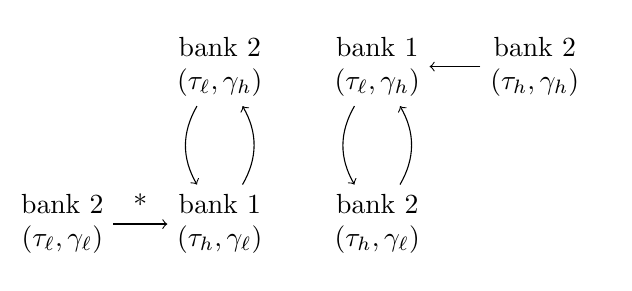
\begin{tikzpicture}
  % Nodes
    \hspace{-0.2cm}\node[align=center] (A) at (-2,0) {bank 2 \\ $(\tau_{\ell},\gamma_{\ell})$};
  \node[align=center] (B) at (0,0) {bank 1 \\ $(\tau_{h},\gamma_{\ell})$};
  \node[align=center] (C) at (2,0) {bank 2\\ $(\tau_{h},\gamma_{\ell})$};
  \node[align=center] (D) at (0,2) {bank 2\\ $(\tau_{\ell},\gamma_{h})$};
  \node[align=center] (E) at (2,2) {bank 1  \\ $(\tau_{\ell},\gamma_{h})$};
  \node[align=center] (F) at (4,2) {bank 2 \\ $(\tau_{h},\gamma_{h})$};
  % Arrows
  \draw[->] (A) -- node[above]{*} (B);
  %\draw[->,red] (D) -- (E);
  %\draw[->,red] (C) -- (B);
  %\draw[->,red] (F) -- (C);
  \draw[->,bend right] (B) to (D);
  \draw[->,bend right] (D) to (B);
  \draw[->,bend right] (E) to (C);
    \draw[->,bend right] (C) to (E);
    \draw[->] (F) to (E);
\end{tikzpicture} 
\caption{$\epsilon_1<0, \epsilon_2>0$.}
\end{minipage}
}
}
\resizebox{0.47\textwidth}{!}{    
\fbox{
\begin{minipage}{0.50\textwidth}
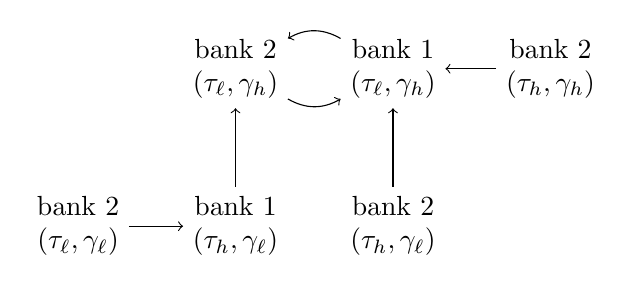
\begin{tikzpicture}
  % Nodes
    \node[align=center] (A) at (-2,0) {bank 2 \\ $(\tau_{\ell},\gamma_{\ell})$};
  \node[align=center] (B) at (0,0) {bank 1 \\ $(\tau_{h},\gamma_{\ell})$};
  \node[align=center] (C) at (2,0) {bank 2\\ $(\tau_{h},\gamma_{\ell})$};
  \node[align=center] (D) at (0,2) {bank 2\\ $(\tau_{\ell},\gamma_{h})$};
  \node[align=center] (E) at (2,2) {bank 1  \\ $(\tau_{\ell},\gamma_{h})$};
  \node[align=center] (F) at (4,2) {bank 2 \\ $(\tau_{h},\gamma_{h})$};
  % Arrows
  \draw[->] (A) -- (B);
  %\draw[->,red] (D) -- (E);
  %\draw[->,red] (C) -- (B);
  %\draw[->,red] (F) -- (C);
  \draw[->] (B) to (D);
  \draw[->] (C) to (E);
  \draw[->,bend right] (D) to (E);
    \draw[->,bend right] (E) to (D);
    \draw[->] (F) to (E);
\end{tikzpicture} 
\caption{$\epsilon_1>0, \epsilon_2>0$.}
\end{minipage}
}
}
\resizebox{0.47\textwidth}{!}{ 
\fbox{
\begin{minipage}{0.5\textwidth}
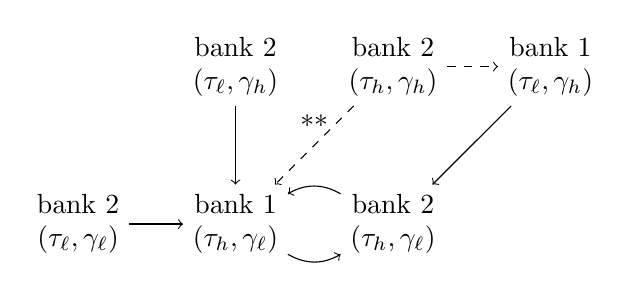
\begin{tikzpicture}
  % Nodes
    \node[align=center] (A) at (-2,0) {bank 2 \\ $(\tau_{\ell},\gamma_{\ell})$};
  \node[align=center] (B) at (0,0) {bank 1 \\ $(\tau_{h},\gamma_{\ell})$};
  \node[align=center] (C) at (2,0) {bank 2\\ $(\tau_{h},\gamma_{\ell})$};
  \node[align=center] (D) at (0,2) {bank 2\\ $(\tau_{\ell},\gamma_{h})$};
  \node[align=center] (E) at (2,2) {bank 2  \\ $(\tau_{h},\gamma_{h})$};
  \node[align=center] (F) at (4,2) {bank 1 \\ $(\tau_{\ell},\gamma_{h})$};
  % Arrows
  \draw[->] (A) -- (B);
  \draw[->] (F) -- (C);
  %\draw[->,red] (D) -- (E);
  %\draw[->,red] (C) -- (B);
  %\draw[->,red] (F) -- (C);
  \draw[->,dashed] (E) -- node[above]{**} (B);
  \draw[->,dashed] (E) -- (F);
  \draw[->] (D) to (B);
  \draw[->,bend right] (B) to (C);
    \draw[->,bend right] (C) to (B);
\end{tikzpicture} 
\caption{$\epsilon_1<0,\epsilon_2<0$.}
\end{minipage}
}
}
\resizebox{0.47\textwidth}{!}{ 
\fbox{
\begin{minipage}{0.5\textwidth}
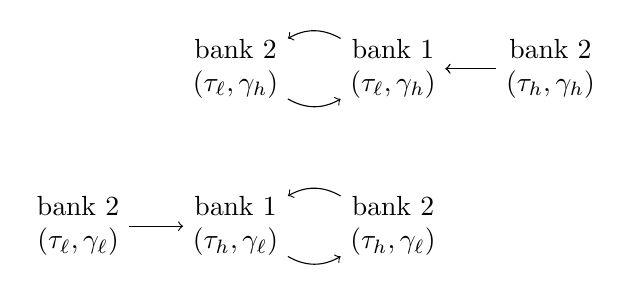
\begin{tikzpicture}
  % Nodes
    \node[align=center] (A) at (-2,0) {bank 2 \\ $(\tau_{\ell},\gamma_{\ell})$};
  \node[align=center] (B) at (0,0) {bank 1 \\ $(\tau_{h},\gamma_{\ell})$};
  \node[align=center] (C) at (2,0) {bank 2\\ $(\tau_{h},\gamma_{\ell})$};
  \node[align=center] (D) at (0,2) {bank 2\\ $(\tau_{\ell},\gamma_{h})$};
  \node[align=center] (E) at (2,2) {bank 1  \\ $(\tau_{\ell},\gamma_{h})$};
  \node[align=center] (F) at (4,2) {bank 2 \\ $(\tau_{h},\gamma_{h})$};
  % Arrows
  \draw[->] (A) -- (B);
  %\draw[->,red] (D) -- (E);
  %\draw[->,red] (C) -- (B);
  %\draw[->,red] (F) -- (C);
  \draw[->] (F) to (E);
  \draw[->,bend right] (B) to (C);
    \draw[->,bend right] (C) to (B);
     \draw[->,bend right] (D) to (E);
    \draw[->,bend right] (E) to (D);
    \draw[->] (F) to (E);
\end{tikzpicture} 
\caption{$\epsilon_1>0, \epsilon_2<0$.}
\end{minipage}
}
}
\caption{Alternative Best Response Dynamics. * The arrows means that, if bank 2 picks decision $(\tau_{\ell},\gamma_{\ell})$, the best response for Bank 1 is $(\tau_{h},\gamma_{\ell})$. ** The dashed arrow means that both case can happen, which depends on specific conditions on $D_y$. Note that it does not have an influence on the final conclusion, since both cases converge to the NE in the end. }
\label{fig:enter-label}
\end{figure}

% \subsection{Proof of Theorem \ref{thm:continous:peq}}
% \label{proof:continous}
% We first introduce the following simple lemma about the properties of $f$, which is easy to check.
% \begin{lemma}
% \label{lem:property of f}
% Assume $\emph{Supp}(D_y)=[0,1]$. We have
% \begin{enumerate}
%     \item $f(\gamma,\tau_a,\tau_b)$ is monotonically increasing with respect to $\gamma$. Moreover, let $y_{\gamma}=\frac{1}{2+\gamma}$, then $f(\gamma,y_{\gamma},\tau)$ is also monotonically increasing with respect to $\gamma$.
%     \item Let $\tau_a<\tau_b<\tau_c$. Then $f_{D_y}(\gamma_1,\tau_a,\tau_c)=f_{D_y}(\gamma_1,\tau_a,\tau_b)+f_{D_y}(\gamma_1,\tau_b,\tau_c)$.
%     \item Let $y_{\gamma}=\frac{1}{2+\gamma}$. If $y_{\gamma}\in(\tau_a,\tau_b)$, then $f(\gamma,\tau_a,y_{\gamma})<0$, and  $f(\gamma,y_{\gamma},\tau_b)>0$. 
% \end{enumerate}   
% \end{lemma}
% \noindent We analyze the existence of pure Nash equilibria under different conditions on the relationship between  decision pairs $\theta_1,\theta_2$. Firstly, note that, for a pair of $\theta_1,\theta_2$,  if the utility of a bank is strictly less than $0$, then the bank can always adjust its parameters $\gamma$ and $\tau$ to $1$ to ensure its utility becomes non-negative. This implies that decision pairs leading to non-positive utilities will not be an Nash equilibrium. Therefore, we only need to consider cases where $u_1 \geq 0$ and $u_2 \geq 0$.



% Next, we discuss the conditions for $\theta_1,\theta_2$ under which there are no pure NE under any distributions. We prove this by showing that, one can always find a new decision $\theta_1'=(\tau'_1,\gamma'_1)$ \textbf{or} $\theta_2'=(\tau'_2,\gamma'_2)$ for Bank 1 or 2 that leads to a larger utility for that bank.

% \paragraph{Case 1:} $\tau_1\leq \tau_2$, and $\gamma_1<\gamma_2$.
% In this case,   $u_1((\tau_1,\gamma_1),(\tau_2,\gamma_2))=f(\gamma_1,\tau_1,1),$ while $u_2=0.$ Let $\gamma_1'=\gamma_1+\epsilon<\gamma_2$ for some $\epsilon>0$. Then, $$u_1((\tau_1,\gamma_1'),(\tau_2,\gamma_2))=f(\gamma'_1,\tau_1,1)>f(\gamma_1,\tau_1,1)=u_1((\tau_1,\gamma_1),(\tau_2,\gamma_2)),$$ 
% where the inequality is based on the first property in Lemma \ref{lem:property of f}. It shows that $(\tau_1,\gamma_1')$ is a better decision for bank 1, therefor this case can not be a NE.   

% \paragraph{Case 2:} $\tau_1<\tau_2,\gamma_1=\gamma_2=\gamma$. In this case, $u_1((\tau_1,\gamma),(\tau_2,\gamma))=f(\gamma,\tau_1,\tau_2)+\frac{1}{2}f(\gamma,\tau_2,1)$, and $u_2((\tau_1,\gamma),(\tau_2,\gamma))=\frac{1}{2}f(\gamma,\tau_2,1)$. If $u_1((\tau_1,\gamma),(\tau_2,\gamma))=0,u_2((\tau_1,\gamma),(\tau_2,\gamma))>0$, then one can set $\tau_1'=\tau_2$, so that $$u_1((\tau_1',\gamma),(\tau_2,\gamma))=u_1((\tau_2,\gamma),(\tau_2,\gamma))=\frac{1}{2}f(\gamma,\tau_2,1)=u_2((\tau_1,\gamma),(\tau_2,\gamma))>0=u_1((\tau_1,\gamma),(\tau_2,\gamma)).$$
% If $u_1((\tau_1,\gamma),(\tau_2,\gamma))=u_2((\tau_1,\gamma),(\tau_2,\gamma))=0$, then it implies that $f(\gamma,\tau_1,\tau_2)=0$. Since $\text{Supp}(D_y)=[0,1]$, it means that there exists $\tau'\in(\tau_1,\tau_2)$ such that $f(\gamma,\tau_1,\tau')<0$ and $f(\gamma,\tau',\tau_2)>0$.  Therefore, if one sets $\tau_2'=\tau'$, we have 
% $$u_2((\tau_1,\gamma),(\tau'_2,\gamma))= f(\gamma,\tau',\tau_2)+\frac{1}{2}f(\gamma,\tau_2,1)>\frac{1}{2}f(\gamma,\tau_2,1)=u_2((\tau_1,\gamma),(\tau_2,\gamma)).$$
% \kri{Check these two subcases below, it's correct but I think some typo}
% If  $u_1((\tau_1,\gamma),(\tau_2,\gamma))>0$, $u_2((\tau_1,\gamma),(\tau_2,\gamma))=0$, it means that $f(\gamma,\tau_1,\tau_2)=0$. On the other hand, since $u_2=\frac{1}{2}f(\gamma,\tau_2,1)=\int_{\tau_2}^1[(2+\gamma)y-1]p(y)dy=0$, there exists a $\tau'\in(\tau_2,1)$, such that $(2+\gamma)\tau'-1=0$. Moreover, for all $\tau<\tau'$,  $(2+\gamma)\tau'-1<0$. This implies that $f(\gamma,\tau_1,\tau_2)<0$. This contradiction means that this case ($u_1((\tau_1,\gamma),(\tau_2,\gamma))>0$, $u_2((\tau_1,\gamma),(\tau_2,\gamma))=0$) will not happen. \\

% \noindent If $u_1((\tau_1,\gamma),(\tau_2,\gamma))>0$, and $u_2((\tau_1,\gamma),(\tau_2,\gamma))>0$, then let $y_{\gamma}=\frac{1}{2+\gamma}$. If $y_{\gamma}\in(\tau_1,\tau_2)$, then we have $f(\gamma,\tau_1,y_{\gamma})<0$, and $f(\gamma,y_{\gamma},\tau_2)>0$. Therefore, if one sets $\tau_1'=y_{\gamma}$, we have 
% $$u_1((\tau'_1,\gamma),(\tau_2,\gamma))=f(\gamma,y_{\gamma},\tau_2)>f(\gamma,\tau_1,y_{\gamma})+f(\gamma,y_{\gamma},\tau_2)=u_1((\tau_1,\gamma),(\tau_2,\gamma)).$$
% If $y_{\gamma}\geq \tau_2$, then we have $f(\gamma,\tau_1,\tau_2)< 0.$ Therefore, if we set $\tau_1'=\tau_2,$ we get 
% $$u_1((\tau_1',\gamma),(\tau_2,\gamma))=\frac{1}{2}f(\gamma,\tau_2,1)>f(\gamma,\tau_1,\tau_2)+\frac{1}{2}f(\gamma,\tau_2,1)>u_1((\tau_1,\gamma),(\tau_2,\gamma)).$$
% Similarly, if $y_{\gamma}\leq \tau_2$, setting $\tau_2'=\tau_1$ leads to a better utility for bank 2. 

% \paragraph{Case 3:} $\tau_1<\tau_2,$ $\gamma_1>\gamma_2$. In this case, $u_1((\tau_1,\gamma_1),(\tau_2,\gamma_2))=f(\gamma_1,\tau_1,\tau_2)$, and $u_2((\tau_1,\gamma),(\tau_2,\gamma))=f(\gamma_2,\tau_2,1)$. Let $y_{\gamma_{1}}=\frac{1}{2+\gamma_1}$, and $y_{\gamma_2}=\frac{1}{2+\gamma_2}$. Then, it is easy to check that if the pair of decisions will not be a NE if $\tau_1\not=y_{\gamma_{1}}$ or $\tau_2\not=y_{\gamma_{2}}$. \kri{We start by observing that for bank $2$ (with lower interest rate), it is optimal to set $\tau_2 = y_{\gamma_2}$ regardless of the other bank. Bank $2$ can always deviate to a threshold $y_{\gamma_2}$ and obtain higher utility, because if $y_{\gamma_2} < \tau_2$, it can drop threshold to $y_{\gamma_2}$ obtaining utility $f(\gamma_2, y_{\gamma_2}, 1) > f(\gamma_2, \tau_2, 1)$, similarly if $\tau_2 < y_{\gamma_2}$, bank 2 can increse threshold to $y_{\gamma_2}$ and get rid of the negative part of the integral}

% For example, if $\tau_1<y_{\gamma_{1}}$, then $f(\gamma_1,\tau_1,y_{\gamma_{1}})<0$, so setting $\tau_1'=y_{\gamma_{1}}$ leads to a larger utility for bank 1. For the case where $\tau_1=y_{\gamma_1}$ and $\tau_2=y_{\gamma_2}$, one can set $\gamma_2'=\gamma_2+\epsilon<\gamma_1$ for some $\epsilon>0$. In this case, 
% $$u_2((\tau_1,\gamma_1),(\tau_2,\gamma'_2))=f(\gamma_2',\tau_2,1)>f(\gamma_2,\tau_2,1)=u_2((\tau_1,\gamma_1),(\tau_2,\gamma_2)).$$


% Next, we discuss the case which can be a NE under certain conditions. 
% \paragraph{Case 4:} $\tau_1=\tau_2=\tau$, and $\gamma_1=\gamma_2=\gamma$. In this case, $u_1((\tau,\gamma),(\tau,\gamma))=u_2((\tau,\gamma),(\tau,\gamma))=\frac{1}{2}f(\gamma,\tau,1)$. Let $y_{\gamma}=\frac{1}{2+\gamma}$. If $y_{\gamma}>\tau$, then $f(\gamma,\tau,y)<0$, so if we sets $\tau'_2=y_{\gamma}$, we have 
% $$ u_2((\tau,\gamma),(\tau',\gamma))=\frac{1}{2}f(\gamma,y_{\gamma},1)>\frac{1}{2}f(\gamma,\tau,y_{\gamma})+\frac{1}{2}f(\gamma,y_{\gamma},1)=u_2((\tau,\gamma),(\tau,\gamma)).$$
% Similarly, if $y_{\gamma}<\tau$, we have $f(\gamma,y_{\gamma},\tau)>0$. Thus, we can set $\tau_2'=y_{\gamma}$, so 
% $$ u_2((\tau,\gamma),(\tau',\gamma))=\frac{1}{2}f(\gamma,y_{\gamma},1)>\frac{1}{2}f(\gamma,\tau,1)=u_2((\tau,\gamma),(\tau,\gamma)).$$
% The above discussion shows that this case will not be an NE if $\tau\not=y_{\gamma}.$ For the case where $\tau=y_{\gamma}$, we consider two possible situations: $\gamma>0$ and $\gamma=0$. If $\gamma>0$, then one can set $\gamma_1'=\gamma-\epsilon$ for a sufficiently small $\epsilon>0$, such that bank one double its profit with a very small cost (provided by $\epsilon$ is sufficiently small). If $\gamma=0$, then $\tau_1=\tau_2=y_{\gamma}=\frac{1}{2}$. In this case, no bank can double the profit by decreasing $\gamma$. Note that the game is symmetric, and the two players in this setting adopt the same decisions. Therefore, the decision pair $(\theta_1=(0.5,0),\theta_2=(0.5,0))$ will be an NE if and only if  
% $$u_1(\theta_1,\theta_2)\geq u_1(\theta'_1=(\tau',\gamma'),\theta_2),$$
% for any other $\theta_1'\in[0,1]^2$. If $\tau'>\tau$ and $\gamma'=\gamma$, then 
% $$u_1((\tau',\gamma'),\theta_2)=\frac{1}{2}f(\gamma,\tau',1)=\frac{1}{2}[f(\gamma,\tau,1) -f(\gamma,\tau,\tau')]<u_1(\theta_1,\theta_2),$$
% since $f(\gamma,\tau,\tau')>0$ by the definition of $y_{\gamma}.$
% If $\tau'<\tau$ and $\gamma'=\gamma$, then 
% $$u_1((\tau',\gamma'),(\tau,\gamma))=\frac{1}{2}f(\gamma,\tau',1)=\frac{1}{2}[f(\gamma,\tau'\tau)+f(\gamma,\tau,1)]<u_1(\theta_1,\theta_2),$$
% as $f(\gamma,\tau',\tau)<0.$ If $\tau'\geq\tau$ and $\gamma'>\gamma$, then $u_1((\tau',\gamma'),\theta_2)=0<u_1((\tau,\gamma),\theta_2)$. Finally, we consider the case where $\tau'<\tau$, and $\gamma'>\gamma$. In this case, 
% $$u_1((\tau',\gamma'),\theta_2)=\int^{\tau}_{\tau'}[(2+\gamma')y-1]p(y)dy.$$
% We have for all $(\tau',\gamma')$ such that $\tau'<\tau$ and $\gamma'>\gamma$, 
% $$\int^{\tau}_{\tau'}[(2+\gamma')y-1]p(y)dy\leq \int^{\tau}_{\tau'}[(2+1)y-1]p(y)dy\leq  \int^{\tau}_{y_1=\frac{1}{2+1}}[(2+1)y-1]p(y)dy=f\left(1,\frac{1}{3},0.5\right).$$
% This implies that, for all $(\tau',\gamma')$ such that $\tau'<\tau$ and $\gamma'>\gamma$, the maximum utility of bank 1 is achieved when $\tau'=\frac{1}{3}$, and $\gamma'=0.5$ \kri{$\gamma' = 1$ right?}. Therefore, $u_1(\theta_1,\theta_2)\geq u_1(\theta'_1=(\tau',\gamma'),\theta_2)$ if and only if 
% $$\frac{1}{2} f(0,0.5,1)\geq f\left(1,\frac{1}{3},0.5\right),$$
% \kri{Edited above}
% which finishes the proof. 



\subsection{Proof of Theorem \ref{thm:mixed-NE}}
\label{Proof:Theorem:mixedNE}
We overload notation and denote the expected utility of bank $i$ under $p_1$ and $p_2$ as:
$$ u_{i}(p_1,p_2)=\E_{\theta_1\sim p_1, \theta_2\sim p_2}[u_i(\theta_1,\theta_2)]. $$


\noindent Firstly, note that, based on Table \ref{tab:my-table} and Lemma \ref{lem:property of f}, it can be easily shown that for any $\theta\in\{\theta^{(j)}\}_{j=1}^4$, 
$$u_1(\theta^{(3)},\theta)> u_1(\theta^{(1)},\theta). $$
More specifically, 
\begin{equation*}
    \begin{split}
u_1(\theta^{(3)},\theta^{(1)})={} & \frac{1}{2}f(\gamma_{\ell},\tau_{h},1)>\frac{1}{2}f(\gamma_{\ell},\tau_{\ell},1) =   u_1(\theta^{(1)},\theta^{(1)}),\\
u_1(\theta^{(3)},\theta^{(2)})={} & f(\gamma_{\ell},\tau_{h},1)>f(\gamma_{\ell},\tau_{\ell},1) =   u_1(\theta^{(1)},\theta^{(2)}),\\
u_1(\theta^{(3)},\theta^{(3)})={} & \frac{1}{2}f(\gamma_{\ell},\tau_{h},1)>f(\gamma_{\ell},\tau_{\ell},\tau_h)+\frac{1}{2}f(\gamma_{\ell},\tau_h,1) =   u_1(\theta^{(1)},\theta^{(3)}),\\
u_1(\theta^{(3)},\theta^{(4)})={} & f(\gamma_{\ell},\tau_{h},1)>f(\gamma_{\ell},\tau_{\ell},1) =   u_1(\theta^{(1)},\theta^{(4)}),
    \end{split}
\end{equation*}
where the first, second and last inequality is because based on Lemma \ref{lem:property of f}, 
$$f(\gamma_{\ell},\tau_{\ell},1)=\underbrace{f(\gamma_{\ell},\tau_{\ell},\tau_{h})}_{<0}+f(\gamma_{\ell},\tau_{h},\tau_{h}),$$
and the third inequality is because $f(\gamma_{\ell},\tau_{\ell},\tau_{h})<0.$ This implies that $\theta^{(1)}$ is strictly dominated by $\theta^{(3)}$, and will not be part of the mixed NE. 


Since the game is symmetric, the same argument holds true for Bank 2, i.e. $u_2(\theta,\theta^{(3)}) > u_2(\theta,\theta^{(1)})$. By a similar argument, for any $\theta\in\{\theta^{(j)}\}_{j=2}^4$, we have
$$u_1(\theta^{(2)},\theta)> u_1(\theta^{(4)},\theta), $$
which indicates that $\theta^{(4)}$ will also not be part of mixed NE for Bank 1 or Bank 2.  To summarize, any mixed NE must satisfy $p_{1,1}=p_{1,4}=p_{2,1}=p_{2,4}=0$.\\


\noindent Consider a pair of mixed strategies $p_1=[0,p_{1,2},1-p_{1,2},0]$ and $p_2=[0,p_{2,2},1-p_{2,2},0]$. Then the utility of Bank 1 can be written as: 
\begin{equation}
    \begin{split}
    \label{eqn:u13123123}
u_{1}(p_1,p_2) = {} & \frac{1}{2} p_{1,2}p_{2,2} f(\gamma_{h}, \tau_{\ell}, 1) + p_{1,2}(1-p_{2,2})f(\gamma_{h},\tau_{\ell},\tau_{h})+ (1-p_{1,2})p_{2,2}f(\gamma_{\ell},\tau_h,1)\\
{} & + \frac{(1-p_{1,2})(1-p_{2,2})}{2}f(\gamma_{\ell},\tau_{h},1)\\       = {} & \frac{1}{2}p_{1,2}\left[(2-p_{2,2})f(\gamma_{h},\tau_{\ell},\tau_{h}) + p_{2,2}f(\gamma_{h},\tau_{h},1) -(1+p_{2,2})f(\gamma_{\ell},\tau_{h},1) \right] \\
{} & + \frac{(p_{2,2}+1)}{2}f(\gamma_{\ell},\tau_{h},1).
    \end{split}
\end{equation}
Note that it is a linear function with respect to $p_{1,2}$, and the slope is given by:
\begin{equation*}
    \begin{split}
        {} & \frac{1}{2} \left[(2-p_{2,2})f(\gamma_{h},\tau_{\ell},\tau_{h}) + p_{2,2}f(\gamma_{h},\tau_{h},1) -(1+p_{2,2})f(\gamma_{\ell},\tau_{h},1)\right]\\
        = {} & \frac{1}{2} p_{2,2}[f(\gamma_{h},\tau_{h},1)-f(\gamma_{\ell},\tau_{h},1)-f(\gamma_{h},\tau_{\ell},\tau_{h})] + f(\gamma_{h},\tau_{\ell},\tau_{h}) - \frac{1}{2} f(\gamma_{\ell},\tau_{h},1),
    \end{split}
\end{equation*}
Let 
\begin{equation}
\label{eqn:def-of-g(p)}
g(p)=p[f(\gamma_{h},\tau_{h},1)-f(\gamma_{\ell},\tau_{h},1)-f(\gamma_{h},\tau_{\ell},\tau_{h})] + 2f(\gamma_{h},\tau_{\ell},\tau_{h}) - f(\gamma_{\ell},\tau_{h},1).
\end{equation}
Then, the slope of $u(p_1,p_2)$ with respect to $p_{1,2}$ is given by $\frac{1}{2} g(p_{2,2})$.
Moreover, (recalling our definitions of the shorthand notation $\epsilon_1 = \frac{1}{2} f(\gamma_h, \tau_{\ell},1) - f(\gamma_{\ell},\tau_h, 1)$ and $\epsilon_2 = f(\gamma_h, \tau_{\ell}, \tau_h) - \frac{1}{2} f(\gamma_{\ell},\tau_h, 1)$), we note that $g(p):[0,1]\mapsto \R$ is a linear function, $g(0)=2\epsilon_2$, and $g(1)=2\epsilon_1$.
\\
\noindent 

Let $BR_1(p) \subseteq [0,1]$ denote the candidate set of best response probabilities of picking $\theta^{(2)}$ of Bank 1 if Bank 2 picks $p_2=[0,p,1-p,0]$. 
The corresponding candidate set for Bank 2 is denoted by $BR_2(p)$.

Then, consider the following cases: 

\noindent \paragraph{Case 1:} $\epsilon_1<0$, $\epsilon_2<0$. Therefore, $g(0)=2\epsilon_2<0$ and  $g(1)=2\epsilon_1<0$, 
then it is clear that $g(p)<0$ for all $p\in[0,1]$. 
This means that the slope in \eqref{eqn:u13123123} will always be negative, so $BR_1(p)= \{0\}$ for any $p\in[0,1]$. Similarly, $BR_2(p)=\{0\}$ for any $p\in[0,1]$, which indicates that $p_{1,2}=p_{2,2}=0$, $p_{1,3}=p_{2,3}=1$ is the only mixed NE (and, in fact, this corresponds to a pure NE).

\noindent \paragraph{Case 2:} $\epsilon_1<0$, $\epsilon_2>0$. Therefore, $g(0)>0$, and $g(1)<0$, and since $g$ is a linear function, it means that there must exist a unique $c\in(0,1)$, such that $g(c)=0$. Based on \eqref{eqn:def-of-g(p)}, we know 
$$ c=\frac{f(\gamma_{\ell},\tau_h,1)-2f(\gamma_h,\tau_{\ell},\tau_h)}{f(\gamma_h,\tau_h,1)-f(\gamma_{\ell},\tau_h,1)-f(\gamma_h,\tau_{\ell},\tau_h)}.$$
Combining with \eqref{eqn:u13123123}, we have 
\begin{equation*}
BR_1(p)= 
    \begin{cases}
        \{0\}, & p>c;\\
        \{1\},  & p<c;\\
        [0,1], & p=c.
    \end{cases}
\end{equation*}
This is because, if $p>c$, $g(p)<0$, so the slope in \eqref{eqn:u13123123} is negative, and $BR_1(p)=\{0\}$.If $p<c$, then $g(p)>0$, the slope in \eqref{eqn:u13123123} is positive, and $BR_1(p)=\{1\}$. If $p=c$, \eqref{eqn:u13123123} will not be a function of $p_{1,2}$, so any decision for Bank 1 leads to the same gain. Similarly, we have 
\begin{equation*}
BR_2(p)= 
    \begin{cases}
        \{0\}, & p>c;\\
        \{1\},  & p<c;\\
        [0,1], & p=c.
    \end{cases}
\end{equation*}
Therefore, we know that $([0,c,1-c,0],[0,c,1-c,0])$ is a mixed NE, and $([0,0,1,0],[0,1,0,0])$ and $([0,1,0,0],[0,0,1,0])$ are also pure NEs. 

\noindent \paragraph{Case 3:} $\epsilon_1>0$, $\epsilon_2<0$. Therefore, $g(0)<0$, and $g(1)>0$, and since $g$ is a linear function, it means that there must exist $c\in(0,1)$, such that $g(c)=0$. 
Combining with \eqref{eqn:u13123123}, we have 
\begin{equation*}
BR_1(p)= 
    \begin{cases}
        \{1\}, & p>c;\\
        \{0\},  & p<c;\\
        [0,1], & p=c.
    \end{cases}
\end{equation*}
Similarly, we have 
\begin{equation*}
BR_2(p)= 
    \begin{cases}
        \{1\}, & p>c;\\
        \{0\},  & p<c;\\
        [0,1], & p=c.
    \end{cases}
\end{equation*}
Therefore, we know that $([0,c,1-c,0],[0,c,1-c,0])$ is a mixed NE, and $([0,0,1,0],[0,0,1,0])$ and $([0,1,0,0],[0,1,0,0])$ are also pure NEs. 

\noindent \paragraph{Case 4:} $\epsilon_1>0$, $\epsilon_2>0$. In this case, we know that $g(p)>0$ for all $p\in[0,1]$. Then, we have $BR_1(p)=\{1\}$, and $BR_2(p)=\{1\}$, which implies that the only mixed NE here is $([0,1,0,0], [0,1,0,0])$ (which is in fact a pure NE).
This completes the proof of the theorem.

\subsection{Proof of Theorem \ref{thm:cE}}
\label{proof:CE}

Firstly, we know $u_i(\theta^{(3)},\theta)> u_i(\theta^{(1)},\theta),$. This means $\theta^{(1)}$ will not be part of CE. Conditioned on this, for any $\theta\in\{\theta^{(j)}\}_{j=2}^4$, we have
$u_1(\theta^{(2)},\theta)> u_1(\theta^{(4)},\theta).$ This indicates that $\theta^{(4)}$ will no be part of CE. Thus, $p_{11}=\dots,=p_{14}=0$, $p_{11}=\dots,=p_{41}=0$, $p_{14}=\dots,=p_{44}=0$, $p_{41}=\dots,=p_{44}=0$. Next, based on Definition \ref{defn:CE}, we firstly need:
\begin{equation*}
    \begin{split}
     \sum_{i=2}^3 u_1\left((\tau_{\ell},\gamma_{h}),\theta^{(i)}\right)p_{2i} \geq {} &    \sum_{i=2}^3 u_1\left(\theta',\theta^{(i)}\right)p_{2i},\ \forall \theta'\in\Theta, 
    \end{split}
\end{equation*}
That is, for $\theta'=\theta^{(1)}$,
\begin{equation*}
    \begin{split}
 p_{22}\frac{1}{2}f(\gamma_h,\tau_{\ell},1) + p_{23} f(\gamma_h,\tau_{\ell},\tau_{h}) \geq  p_{22} f(\gamma_{\ell},\tau_{\ell},1) + p_{23} (f(\gamma_{\ell},\tau_{\ell},\tau_h)+\frac{1}{2}f(\gamma_{\ell},\tau_h,1)),     
    \end{split}
\end{equation*}
that is, 
$$ p_{22}(\epsilon_1-f(\gamma_{\ell},\tau_{\ell},\tau_h) )\geq p_{23}(f(\gamma_{\ell},\tau_{\ell},\tau_h)-\epsilon_2  ),$$
that is 
\begin{equation}
\label{eqn:ce:drop1}
    p_{22}\epsilon_1 \geq -p_{23}\epsilon_2 + (p_{22}+p_{23})f(\gamma_{\ell},\tau_{\ell},\tau_h). 
\end{equation}
For $\theta'=\theta^{(3)}$, we have 
\begin{equation}
\label{eqn:ce:nodrop1}
     p_{22}\epsilon_1 \geq  -p_{23}\epsilon_2.
\end{equation}
Note that since 
$f(\gamma_{\ell},\tau_{\ell},\tau_h)$ is negative, we know that \eqref{eqn:ce:nodrop1} implies \eqref{eqn:ce:drop1}, and thus \eqref{eqn:ce:drop1} can be dropped. 

For $\theta'=\theta^{(4)}$, we have 
\begin{equation*}
    \begin{split}
 p_{22}\frac{1}{2}f(\gamma_h,\tau_{\ell},1) + p_{23} f(\gamma_h,\tau_{\ell},\tau_{h}) \geq  p_{22} \frac{1}{2}f(\gamma_{h},\tau_h,1) + p_{23} 0,     
    \end{split}
\end{equation*}
which always holds true. Next, we need 
\begin{equation*}
    \begin{split}
     \sum_{i=2}^3 u_1\left((\tau_{h},\gamma_{\ell}),\theta^{(i)}\right)p_{3i} \geq {} &    \sum_{i=2}^3 u_1\left(\theta',\theta^{(i)}\right)p_{3i},\ \forall \theta'\in\Theta. 
    \end{split}
\end{equation*}
For $\theta'=\theta^{(1)}$, it means 
$$p_{32} f(\gamma_{\ell},\tau_{h},1) + p_{33}\frac{1}{2}f(\gamma_{\ell},\tau_h,1)\geq p_{32} f(\gamma_{\ell},\tau_{\ell},1) + p_{33} \left(f(\gamma_{\ell},\tau_{\ell},\tau_h)+\frac{1}{2}f(\gamma_{\ell},\tau_h,1)\right), $$
which always holds true. For $\theta'=\theta^{(2)}$, we have 
$$ -p_{32}\epsilon_1\geq p_{33}\epsilon_2.$$
For $\theta'=\theta^{(4)}$, we have 
$$ p_{32} f(\gamma_{\ell},\tau_{h},1) + p_{33}\frac{1}{2}f(\gamma_{\ell},\tau_h,1) \geq p_{32} \frac{1}{2} f(\gamma_{h},\tau_h,1). $$
Rearrange, we have
$$ -p_{32}\epsilon_1\geq p_{33}\epsilon_2 -\left(p_{33}+\frac{1}{2}p_{32}\right)f(\gamma_{h},\tau_{\ell},\tau_h). $$
Since $f(\gamma_{h},\tau_{\ell},\tau_h)$ is positive, the above condition is implied by $ -p_{32}\epsilon_1\geq p_{33}\epsilon_2,$ and thus can be dropped. 

To proceed, we need 
\begin{equation*}
    \begin{split}
     \sum_{i=2}^3 u_2\left(\theta^{(i)},(\tau_{\ell},\gamma_{h})\right)p_{i2} \geq {} &    \sum_{i=2}^3 u_2\left(\theta^{(i)},\theta'\right)p_{i2},\ \forall \theta'\in\Theta, 
    \end{split}
\end{equation*}
which is equivalent to 
\begin{equation*}
    \begin{split}
     \sum_{i=2}^3 u_1\left((\tau_{\ell},\gamma_{h}),\theta^{(i)}\right)p_{i2} \geq {} &    \sum_{i=2}^3 u_1\left(\theta',\theta^{(i)}\right)p_{i2},\ \forall \theta'\in\Theta. 
    \end{split}
\end{equation*}
Thus, following similar procedure, the condition we get is 
$$ p_{22}\epsilon_1\geq -p_{32}\epsilon_2. $$
Finally, for 
\begin{equation*}
    \begin{split}
     \sum_{i=2}^3 u_2\left(\theta^{(i)},(\tau_{h},\gamma_{\ell})\right)p_{i3} \geq {} &    \sum_{i=2}^3 u_2\left(\theta^{(i)},\theta'\right)p_{i3},\ \forall \theta'\in\Theta, 
    \end{split}
\end{equation*}
we get 
$$ -p_{23}\epsilon_1\geq p_{33}\epsilon_2,$$
To summarize, we have the following conditions:
\begin{align}
        p_{22}\epsilon_1 \geq {} & -p_{23}\epsilon_2 \label{eq:first}\\
        -p_{32}\epsilon_1\geq {} & p_{33}\epsilon_2 \label{eq:second}.\\
        p_{22}\epsilon_1\geq {} & -p_{32}\epsilon_2 \label{eq:fourth}\\
         -p_{23}\epsilon_1\geq {} & p_{33}\epsilon_2 \label{eq:fifth},
\end{align}
When $\epsilon_1>0$ and $\epsilon_2>0$, from \eqref{eq:second} and \eqref{eq:fifth}, we know that $p_{32}=p_{33}=p_{23}=0$, which leads to $p_{22}=1$, and it can make sure all inequality is ture. Similarly,  when $\epsilon_1<0$ and $\epsilon_2<0$, we get $p_{22}=p_{32}=p_{23}=0$, and $p_{33}=1$.

When $\epsilon_1>0,\epsilon_2<0$,  we need $\min\{p_{22},p_{33}\}>\max\left\{ \frac{|\epsilon_2|}{\epsilon_1}p_{23}, \frac{\epsilon_1}{|\epsilon_2|}p_{32} \right\}$. For  $\epsilon_1<0$ and $\epsilon_2>0$, we need $\min\{p_{23},p_{32}\}>\max\left\{ \frac{|\epsilon_1|}{\epsilon_2}p_{22}, \frac{\epsilon_2}{|\epsilon_1|}p_{33} \right\}$. 




\section{Proofs for Section~\ref{sec:learntoconvege}: Convergence of Dynamics}



\subsection{Proof of Lemma \ref{lem:1 and 4 p}}
\label{proof:Lemma: converofp_1p_4}
We have for $t>1$,
\begin{equation*}
\begin{split}
    \frac{p^{(t+1)}_{1,1}}{p^{(t+1)}_{1,3}}  = {} & \frac{p^{(t)}_{1,1}\exp\left(\eta \sum_{j=1}^4 p_{2,j}^{(t)}u_1\left(\theta^{(1)},\theta^{(j)}\right) \right)}{p^{(t)}_{1,3}\exp\left(\eta \sum_{j=1}^4 p_{2,j}^{(t)}u_1\left(\theta^{(3)},\theta^{(j)}\right) \right)} = \frac{p_{1,1}^{(t)}}{p_{1,3}^{(t)}}\exp\left(\eta \sum_{j=1}^4p_{2,j}^{(t)}\left(u_1\left(\theta^{(1)},\theta^{(j)}\right)-u_1\left(\theta^{(3)},\theta^{(j)}\right)\right)\right) \\
\leq {} &  \frac{p_{1,1}^{(t)}}{p_{1,3}^{(t)}}\exp\left(-\eta\xi_1\right),
\end{split}
\end{equation*}
where recall that we defined $\xi_1 := \min\{\frac{1}{2}\left|f(\gamma_{\ell},\tau_{\ell},\tau_{h})\right|,\frac{1}{2}|f(\gamma_{h},\tau_{\ell},\tau_{h})|, |\epsilon_1|, |\epsilon_2|\}>0$ as shorthand.
Therefore, we have 
\[
{p^{(t+1)}_{1,1}}\leq p_{1,3}^{(t+1)} \frac{p^{(1)}_{1,1}}{p^{(1)}_{1,3}}\left[\exp\left(-\eta\xi_1\right)\right]^{t}\leq  \frac{p^{(1)}_{1,1}}{p^{(1)}_{1,3}}\left[\exp\left(-\eta\xi_1\right)\right]^{t}\leq c_{ini}\left[\exp\left(-\eta\xi_1\right)\right]^{t},
\]
where the last inequality plugs in the definition of $c_{ini}=\max_{i\in[2]}\left\{\frac{\max_{j\in[4]}p^{(1)}_{i,j}}{\min_{i\in[4]}p^{(1)}_{i,j}}\right\}$.
Similarly, we also have 

\begin{equation*}
\begin{split}
    \frac{p^{(t+1)}_{2,1}}{p^{(t+1)}_{2,3}}  = {} & \frac{p^{(t)}_{2,1}\exp\left(\eta \sum_{j=1}^4 p_{1,j}^{(t)}u_2\left(\theta^{(j)},\theta^{(1)}\right) \right)}{p^{(t)}_{2,3}\exp\left(\eta \sum_{j=1}^4 p_{1,j}^{(t)}u_2\left(\theta^{(j)},\theta^{(3)}\right) \right)} = \frac{p_{2,1}^{(t)}}{p_{2,3}^{(t)}}\exp\left(\eta \sum_{j=1}^4p_{1,j}^{(t)}\left(u_1\left(\theta^{(1)},\theta^{(j)}\right)-u_1\left(\theta^{(3)},\theta^{(j)}\right)\right)\right) \\
\leq {} &  \frac{p_{2,1}^{(t)}}{p_{2,3}^{(t)}}\exp\left(-\eta\xi_1\right),
\end{split}
\end{equation*}
where the second equality is based on the fact the game is symmetric. It implies that 
\[
{p^{(t+1)}_{2,1}}\leq c_{ini}\left[\exp\left(-\eta\xi_1\right)\right]^{t}.
\]
Next, we know that $u_1(\theta^{(2)},\theta^{(1)})=u_1(\theta^{(4)},\theta^{(1)})=0$, but for all $j \neq 1$, we have $u_1\left(\theta^{(2)},\theta^{(j)}\right) - u_1\left(\theta^{(4)},\theta^{(j)}\right) \geq \xi_1$. Therefore, we have for all $t>1$,
\begin{equation}\label{eq:recursive-p14}
   \begin{split}
\frac{p^{(t+1)}_{1,4}}{p^{(t+1)}_{1,2}} =      \frac{p^{(t)}_{1,4}}{p^{(t)}_{1,2}} \exp\left(\eta \sum_{j=2}^4 p^{(t)}_{2,j}\left(u_1\left(\theta^{(4)},\theta^{(j)}\right)-u_1\left(\theta^{(2)},\theta^{(j)}\right)\right) \right)\leq \frac{p^{(t)}_{1,4}}{p^{(t)}_{1,2}} \exp\left(-\eta \xi_1\sum_{j=2}^4 p^{(t)}_{2,j} \right).
   \end{split} 
\end{equation}
Note that it implies that the ratio between $p_{1,4}^{(t)}$ and $p_{1,2}^{(t)}$ is non-increasing. Moreover, we have just shown that
\[
p_{2,1}^{(t)}\leq c_{ini}\exp\left(-\eta\xi_1(t-1)\right)
\]
For $t\geq t'=\max\left\{\left\lceil\frac{\log 2c_{ini}}{\epsilon\eta}+1\right\rceil,2\right\}$, we have $p_{2,1}^{(t)}\leq \frac{1}{2}$, which implies that 
\[
\sum_{j=2}^4p_{2,j}^{(t)}= 1- p_{1,2}^{(t)}\geq\frac{1}{2}.
\] 
Thus, 
\begin{equation*}
    \begin{split}
 \frac{p^{(t+1)}_{1,4}}{p^{(t+1)}_{1,2}}\leq {} &  \frac{p^{(t)}_{1,4}}{p^{(t)}_{1,2}} \exp\left(-\eta \xi_1\sum_{j=2}^4 p^{(t)}_{2,j} \right)\leq \frac{p^{(t'-1)}_{1,4}}{p^{(t'-1)}_{1,2}} \left(\exp\left(-\frac{1}{2}\eta \xi_1 \right)\right)^{t-t'+1}\exp\left(-\eta\xi_1\sum_{j=2}^4p_{2,j}^{(t'-1)}\right)\\
\leq {} &\frac{p^{(1)}_{1,4}}{p^{(1)}_{1,2}} \left(\exp\left(-\frac{1}{2}\eta \xi_1 \right)\right)^{t-t'+1}\leq c_{ini}\exp\left(-\frac{1}{2}\eta \xi_1(t-t'+1) \right).       
    \end{split}
\end{equation*}
where the penultimate inequality uses Equation~\eqref{eq:recursive-p14} recursively for $t = t' - 1, \ldots, 1$. We complete the proof by setting 
$$c_{ini}\exp\left(-\frac{1}{2}\eta \xi_1(t-t'+1) \right)\leq\omega. $$

%This completes the proof of the lemma.

\subsection{Proof of Theorem 4}
\label{proof:Theoerm:conveccc}
In this section, we present the proof of Theorem 4, considering four cases based on the different possible signs of $\epsilon_1$ and $\epsilon_2$.\\
Recall the definitions $\epsilon_1 = \frac{1}{2} f(\gamma_h, \tau_{\ell},1) - f(\gamma_{\ell},\tau_h, 1)$ and $\epsilon_2 = f(\gamma_h, \tau_{\ell}, \tau_h) - \frac{1}{2} f(\gamma_{\ell},\tau_h, 1)$.
Also recall the shorthand definitions $\xi_1=\min\{\frac{1}{2}f(\gamma_{\ell},\tau_{h},1), \frac{1}{2}\left|f(\gamma_{\ell},\tau_{\ell},\tau_{h})\right|,\frac{1}{2}|f(\gamma_{h},\tau_{\ell},\tau_{h})|, |\epsilon_1|, |\epsilon_2|\}>0$ and $c_{ini} := \max_{i\in[2]}\left\{\frac{\max_{j\in[4]}p^{(1)}_{i,j}}{\min_{i\in[4]}p^{(1)}_{i,j}}\right\}$.


\noindent \textbf{Case I: $\epsilon_1<0,$ and $\epsilon_2<0$.} We have 
\begin{equation}
    \begin{split}
    \label{eqn:throrem 4:case1}
     \frac{p^{(t+1)}_{1,2}}{p^{(t+1)}_{1,3}}  = {} &  \frac{p^{(t)}_{1,2}}{p^{(t)}_{1,3}}\exp\left(\eta \sum_{j=1}^4 p^{(t)}_{2,j}\left(u_1\left(\theta^{(2)}, \theta^{(j)}\right)-u_1\left(\theta^{(3)}, \theta^{(j)}\right)\right)\right) \\ 
     \leq  {} &  \frac{p^{(t)}_{1,2}}{p^{(t)}_{1,3}}\exp\left( -\eta \sum_{j=1}^3p^{(t)}_{2,j}\xi_1 + p^{(t)}_{2,4}\left(f(\gamma_{h},\tau_{\ell},\tau_{h})+\frac{1}{2}f(\gamma_{h},\tau_{h},1)-f(\gamma_{\ell},\tau_h,1)\right)  \right)\\
     \leq {} &  \frac{p^{(t)}_{1,2}}{p^{(t)}_{1,3}}\exp\left( -\eta \sum_{j=1}^3p^{(t)}_{2,j}\xi_1 + 3\eta p^{(t)}_{2,4}  \right)
     =  \frac{p^{(t)}_{1,2}}{p^{(t)}_{1,3}}\exp\left( -\eta \sum_{j=1}^4p^{(t)}_{2,j}\xi_1 + \eta(\xi_1+3) p^{(t)}_{2,4}  \right)\\
     = {} &  \frac{p^{(t)}_{1,2}}{p^{(t)}_{1,3}}\exp\left( -\eta\xi_1 + \eta(\xi_1+3) p^{(t)}_{2,4}  \right).\\
    \end{split}
\end{equation}
For the first inequality, it is because:
\begin{equation*}
    \begin{split}
u_1(\theta^{(2)},\theta^{(1)})-u_1(\theta^{(3)},\theta^{(1)})={} & 0-\frac{1}{2}f(\gamma_{\ell},\tau_{h},1)\leq -\xi_1,\\
u_1(\theta^{(2)},\theta^{(2)})-u_1(\theta^{(3)},\theta^{(2)})={} & \frac{1}{2}f(\gamma_{h},\tau_{\ell},1)-f(\gamma_{\ell},\tau_{h},1)=\epsilon_1\leq -\xi_1,\\
u_1(\theta^{(2)},\theta^{(3)})-u_1(\theta^{(3)},\theta^{(3)})={} &f(\gamma_{h},\tau_{\ell},\tau_{h})- \frac{1}{2}f(\gamma_{\ell},\tau_{h},1)=\epsilon_2\leq -\xi_1.
    \end{split}
\end{equation*}
The second inequality of \eqref{eqn:throrem 4:case1} is because the $f$ function is upper bounded by 2 based on Lemma \ref{lem:property of f}, and $f(\gamma_{\ell},\tau_{h},1)$ is positive. Denote as shorthand the constant $t''=t'+1+\left\lceil\frac{2}{\eta\xi_1}\log\frac{2(\xi_1+3)c_{ini}}{\xi_1}\right\rceil$.
Then, from Lemma \ref{lem:1 and 4 p}, we have for $t\geq t''$, 
$$\eta(\xi_1+3)p_{2,4}^{(t)}\leq \frac{\eta\xi_1}{2}.$$
Thus, we have  
\begin{equation*}
    \begin{split}
   \frac{p^{(t+1)}_{1,2}}{p^{(t+1)}_{1,3}} 
   \leq {} & \frac{p^{(t)}_{1,2}}{p^{(t)}_{1,3}} \exp\left(-\frac{\eta\xi_1}{2}\right) \ldots \leq \frac{p^{(t''-1)}_{1,2}}{p^{(t''-1)}_{1,3}} \left[\exp\left(-\frac{\eta\xi_1}{2}\right)\right]^{t-t''+1}\\
   \leq {} & c_{\text{ini}}\exp\left(3\eta t''\right)\exp\left(-\frac{\eta\xi_1}{2}\left(t-t''+1\right)\right),     
    \end{split}
\end{equation*}
where the last inequality is obtained by applying the following inequality recursively for $t=t''-1,\dots,1$:
$$  \frac{p^{(t)}_{1,2}}{p^{(t)}_{1,3}}  \leq  \frac{p^{(t-1)}_{1,2}}{p^{(t-1)}_{1,3}}\exp\left( -\eta\xi_1 + \eta(\xi_1+3) p^{(t-1)}_{2,4}  \right)\leq \frac{p^{(t-1)}_{1,2}}{p^{(t-1)}_{1,3}} \exp(3\eta),$$
which is obtained based on \eqref{eqn:throrem 4:case1}.

Note that $t''$ is a constant. We have for $t\geq t''$,
$$p^{(t+1)}_{1,2}\leq c_{\text{ini}}\exp\left(3\eta t''\right)\exp\left(-\frac{\eta\xi_1}{2}\left(t-t''+1\right)\right), $$ 
and thus 
$$ p^{(t+1)}_{1,3}\geq \max\left\{ 1 -3c_{\text{ini}}\exp\left(3\eta t''\right)\exp\left(-\frac{\eta\xi_1}{2}\left(t-t''+1\right)\right),0\right\} $$
The proof is completed by setting 
$$c_{\text{ini}}\exp\left(3\eta t''\right)\exp\left(-\frac{\eta\xi_1}{2}\left(t-t''+1\right)\right)\leq \omega.$$
It shows that $p_{1,2}^{(t)}$ converges to 0 at an exponential rate after $t''$ iterations, which is a constant factor. Combining with Lemma \ref{lem:1 and 4 p}, we can draw the conclusion that $p_{1,3}^{(t)}$ converges to 1 exponentially fast after a constant number of iterations.
An identical argument reaches the same conclusion for Bank 2.
This implies that the algorithm eventually converges to the symmetric pure NE $((\tau_h, \gamma_{\ell}),(\tau_h, \gamma_{\ell}))$.
\\


\noindent \textbf{Case II: $\epsilon_1>0,$ and $\epsilon_2>0$.} 
The proof for this case proceeds similarly to Case I.
We have:
\begin{equation}
    \begin{split}
    \label{eqn:case2:1113112}
\frac{p^{(t+1)}_{1,3}}{p^{(t+1)}_{1,2}} = {} & \frac{p^{(t)}_{1,3}}{p^{(t)}_{1,2}}\exp\left( \eta \sum_{j=1}^4p^{(t)}_{2,j}\left(u_1\left(\theta^{(3)}, \theta^{(j)}\right)-u_1\left(\theta^{(2)}, \theta^{(j)}\right)\right) \right) \\
\leq {} & \frac{p^{(t)}_{1,3}}{p^{(t)}_{1,2}}\exp\left( -\eta \sum_{j=2}^4p^{(t)}_{2,j}\xi_1   + \eta p^{(t)}_{2,1} \right)
=  \frac{p^{(t)}_{1,3}}{p^{(t)}_{1,2}}\exp\left( -\eta \sum_{j=1}^4p^{(t)}_{2,j}\xi_1   + \eta(1+\xi_1)  p^{(t)}_{2,1}\right).
    \end{split}
\end{equation}
where the first inequality is because 
\begin{equation*}
   \begin{split}
    u_1(\theta^{(3)},\theta^{(2)}) - u_1(\theta^{(2)},\theta^{(2)}) = {} &-\epsilon_1\leq -\xi_1, \\
      u_1(\theta^{(3)},\theta^{(3)}) - u_1(\theta^{(2)},\theta^{(3)}) ={} & -\epsilon_2\leq -\xi_1, \\
      u_1(\theta^{(3)},\theta^{(4)}) - u_1(\theta^{(2)},\theta^{(4)}) ={} & f(\gamma_{\ell},\tau_{h},1) - f(\gamma_{h},\tau_{\ell},\tau_{h})-\frac{1}{2} f(\gamma_{h},\tau_{h},1)\\
      \leq {} & f(\gamma_{\ell},\tau_{h},1) - \frac{1}{2}f(\gamma_{h},\tau_{\ell},\tau_{h})-\frac{1}{2} f(\gamma_{h},\tau_{h},1)\\
      = {} & f(\gamma_{\ell},\tau_{h},1) - \frac{1}{2}f(\gamma_{h},\tau_{\ell},1)=-\epsilon_1\leq -\xi_1
   \end{split} 
\end{equation*}


Denote as shorthand the constant $t'''=\left\lceil\frac{1}{\eta\xi_1}\log\frac{2(1+\xi_1)c_{\text{ini}}}{\xi_1}\right\rceil+1$.
Then, again using Lemma~\ref{lem:1 and 4 p}, we have for all $t \geq t'''$:
$$ \eta(1+\xi_1)p_{2,1}^{(t)}\leq \frac{\eta\xi_1}{2}, $$
In this case, i.e., for $t\geq t'''$, we have 
\begin{align*}
    \frac{p^{(t+1)}_{1,3}}{p^{(t+1)}_{1,2}} \leq \frac{p^{(t)}_{1,3}}{p^{(t)}_{1,2}} \exp\left(-\frac{\eta\xi_1}{2}\right) \ldots &\leq \frac{p^{(t'''-1)}_{1,3}}{p^{(t'''-1)}_{1,2}} \exp\left(-\frac{\eta\xi_1}{2}(t-t'''+1)\right)
    \\& \leq c_{\text{ini}}\exp(t'''\eta)\exp\left(-\frac{\eta\xi_1}{2}(t-t'''+1)\right)\leq \omega. 
\end{align*}
%\vidya{can you replace all appearances of $\left[\exp\left(-\frac{\eta \xi_1}{2}\right)\right]^t$ with $\exp\left(- \frac{\eta \xi_1 t}{2}\right)$? The latter is easier to read/format.}
It shows that $p_{1,3}^{(t+1)}$ converges to 0 exponentially fast after $t'''$, which is a constant factor. Combining with Lemma \ref{lem:1 and 4 p}, we can draw the conclusion that $p_{1,2}^{(t)}$ converges to 1 exponentially fast after a constant number of iterations. 
An identical argument reaches the same conclusion for Bank 2.
This implies that the algorithm eventually converges to the symmetric pure NE $((\tau_{\ell},\gamma_h),(\tau_{\ell},\gamma_h))$.\\

\noindent \textbf{Case III: $\epsilon_1<0,$ and $\epsilon_2>0$.}
Note that according to Lemma \ref{lem:1 and 4 p} and the analysis above, we know that $p^{(t)}_{1,1}$ and $p^{(t)}_{1,4}$ converge to 0 exponentially fast under any conditions, and has little influence on the final results. For now, for the simplicity of the proof, we assume $p^{(t)}_{1,1}=p^{(t)}_{1,4}=0$ for $t\geq1$. This can be understood as starting after an initial phase where $p^{(t)}_{1,1}$ and $p^{(t)}_{1,4}$ decrease near to 0. 
%\vidya{don't think we'll have time to do this for EC but it would be good to formalize this a bit more before the arxiv deadline. in particular we expect the proofs to go through if $p^{(t)}_{1,1}, p^{(t)}_{1,4} \leq \delta$ for some small enough $\delta$?}
\\


%We find that the convergence of the algorithm under this case is related to the algorithm initialization. 

%where two cases, where in the first case  $p^{(1)}_{2,2}\epsilon_1+p^{(1)}_{2,3}\epsilon_2$ and $p^{(1)}_{1,2}\epsilon_1+p^{(1)}_{1,3}\epsilon_2$ have different signs (we call it asymmetric initialization), and in the second case the two have the same sign (we call it symmetric initialization). 
For this case we need to assume an \emph{asymmetric} initialization, where $p^{(1)}_{2,2}\epsilon_1+p^{(1)}_{2,3}\epsilon_2$ and $p^{(1)}_{1,2}\epsilon_1+p^{(1)}_{1,3}\epsilon_2$ have different signs. Without loss of generality, first assume $p^{(1)}_{2,2}\epsilon_1+p^{(1)}_{2,3}\epsilon_2<-\Delta$, and $p^{(1)}_{1,2}\epsilon_1+p^{(1)}_{1,3}\epsilon_2>\Delta$, for some constant $\Delta>0$. 
We have for $t=1$,  
\begin{equation*}
    \begin{split}
\frac{p^{(2)}_{1,2}}{p^{(2)}_{1,3}} = \frac{p^{(1)}_{1,2}}{p^{(1)}_{1,3}}\exp\left(\eta\left(p^{(1)}_{2,2}\epsilon_1 + p^{(1)}_{2,3}\epsilon_2\right)\right) \leq   \frac{p^{(1)}_{1,2}}{p^{(1)}_{1,3}}\exp(-\eta\Delta).,
    \end{split}
\end{equation*}
where the last inequality plugs in our initialization condition.
Note that since $p^{(t)}_{1,2}+p^{(t)}_{1,3}=1$ for all $t$, the deceasing of the ratio means that $p^{(2)}_{1,2}< p^{(1)}_{1,2}$, and $p^{(2)}_{1,3}> p^{(1)}_{1,3}$. On the other hand, 
\begin{equation*}
    \begin{split}
\frac{p^{(2)}_{2,3}}{p^{(2)}_{2,2}} = \frac{p^{(1)}_{2,3}}{p^{(1)}_{2,2}}\exp\left(-\eta\left(p^{(1)}_{1,2}\epsilon_1 + p^{(1)}_{1,3}\epsilon_2\right)\right) \leq   \frac{p^{(1)}_{2,3}}{p^{(1)}_{2,2}}\exp(-\eta \Delta). 
    \end{split}
\end{equation*}
Similar to our reasoning for Bank 1, this implies that $p^{(2)}_{2,3}<p^{(1)}_{2,3}$, and $p^{(2)}_{2,2}>p^{(1)}_{2,2}$. 
% Consequently, noting that $\epsilon_1 < 0$ and $\epsilon_2 > 0$ we have $p_{1,2}^{(2)}\epsilon_1 + p_{1,3}^{(2)} \epsilon_2 > p_{1,2}^{(1)} \epsilon_1 + p_{1,3}^{(1)} \epsilon_2$ and $p_{2,2}^{(2)} \epsilon_1 + p_{2,3}^{(2)} \epsilon_2 < p_{2,2}^{(1)} \epsilon_1 + p_{2,3}^{(1)} \epsilon_2$.
We now show that $p^{(t+1)}_{1,2}< p^{(1)}_{1,2}$,  $p^{(t+1)}_{1,3}> p^{(1)}_{1,3}$, $p^{(t+1)}_{2,3}<p^{(1)}_{2,3}$, and $p^{(t+1)}_{2,2}>p^{(1)}_{2,2}$ through an inductive argument.
Assume at $t\geq 2$, $p^{(t)}_{1,2}< p^{(1)}_{1,2}$,  $p^{(t)}_{1,3}> p^{(1)}_{1,3}$, $p^{(t)}_{2,3}<p^{(1)}_{2,3}$, and $p^{(t)}_{2,2}>p^{(1)}_{2,2}$.
Then, noting that $\epsilon_1 < 0$ and $\epsilon_2 > 0$, we have:
\[
  \frac{p^{(t+1)}_{1,2}}{p^{(t+1)}_{1,3}} = \frac{p^{(t)}_{1,2}}{p^{(t)}_{1,3}}\exp\left(\eta\left(p^{(t)}_{2,2}\epsilon_1 + p^{(t)}_{2,3}\epsilon_2\right)\right) \leq \frac{p^{(t)}_{1,2}}{p^{(t)}_{1,3}}\exp\left(\eta\left(p^{(1)}_{2,2}\epsilon_1 + p^{(1)}_{2,3}\epsilon_2\right)\right)\leq \frac{p^{(t)}_{1,2}}{p^{(t)}_{1,3}}\exp(-\eta \Delta),
\]
and 
\[
  \frac{p^{(t+1)}_{2,3}}{p^{(t+1)}_{2,2}} = \frac{p^{(t)}_{2,3}}{p^{(t)}_{2,2}}\exp\left(-\eta\left(p^{(t)}_{1,2}\epsilon_1 + p^{(t)}_{1,3}\epsilon_2\right)\right) \leq \frac{p^{(t)}_{2,3}}{p^{(t)}_{2,2}}\exp\left(-\eta\left(p^{(1)}_{1,2}\epsilon_1 + p^{(1)}_{1,3}\epsilon_2\right)\right)\leq \frac{p^{(t)}_{2,3}}{p^{(t)}_{2,2}}\exp(-\eta \Delta),
\]
which implies that we have $p^{(t+1)}_{1,2}< p^{(1)}_{1,2}$,  $p^{(t+1)}_{1,3}> p^{(1)}_{1,3}$, $p^{(t+1)}_{2,3}<p^{(1)}_{2,3}$, and $p^{(t+1)}_{2,2}>p^{(1)}_{2,2}$, which finishes the induction. This also implies that 
\[
p^{(t+1)}_{1,2}\leq p^{(t+1)}_{1,3}c_{ini}\exp(-\eta  \Delta t), \quad \text{and} \quad p^{(t+1)}_{2,3}\leq p^{(t+1)}_{2,2}c_{ini}\exp(-\eta  \Delta t).
\]





Then we have 
\[
p^{(t+1)}_{1,2}\geq \frac{1}{1+c_{ini}\exp\left(-\eta\Delta t\right)},\ \ \text{and}\ \ p^{(t+1)}_{2,3}\geq \frac{1}{1+c_{ini}\exp\left(-\eta\Delta t\right)},
\]
which implies that the algorithm converges to the asymmetric NE $((\tau_{\ell},\gamma_{h}),(\tau_{h},\gamma_{\ell}))$. 

Finally, consider the other case, i.e., $p^{(1)}_{2,2}\epsilon_1+p^{(1)}_{2,3}\epsilon_2>\Delta$, and $p^{(1)}_{1,2}\epsilon_1+p^{(1)}_{1,3}\epsilon_2<-\Delta$, for some constant $\Delta>0$. The proof proceeds very similarly as to the previous case, but the algorithm will converge to a different NE. We have for $t=1$: 

\begin{equation*}
    \begin{split}
\frac{p^{(2)}_{2,2}}{p^{(2)}_{2,3}} = \frac{p^{(1)}_{2,2}}{p^{(1)}_{2,3}}\exp\left(\eta\left(p^{(1)}_{1,2}\epsilon_1 + p^{(1)}_{1,3}\epsilon_2\right)\right) \leq   \frac{p^{(1)}_{2,2}}{p^{(1)}_{2,3}}\exp(-\eta\Delta),  
    \end{split}
\end{equation*}
and 
\begin{equation*}
    \begin{split}
\frac{p^{(2)}_{1,3}}{p^{(2)}_{1,2}} = \frac{p^{(1)}_{1,3}}{p^{(1)}_{1,2}}\exp\left(-\eta\left(p^{(1)}_{2,2}\epsilon_1 + p^{(1)}_{2,3}\epsilon_2\right)\right) \leq   \frac{p^{(1)}_{1,3}}{p^{(1)}_{1,2}}\exp(-\eta \Delta). 
    \end{split}
\end{equation*}
Therefore, $p_{2,2}^{(2)}< p_{2,2}^{(1)}$,  $p_{1,3}^{(2)}< p_{1,3}^{(1)}$. Assume for $t\geq 2$, $p_{2,2}^{(t)}< p_{2,2}^{(1)}$,  $p_{1,3}^{(t)}< p_{1,3}^{(1)}$,  $p_{2,3}^{(t)}> p_{2,3}^{(1)}$,  $p_{1,2}^{(t)}> p_{1,2}^{(1)}$. 
Then, noting that $\epsilon_1 < 0$ and $\epsilon_1 > 0$, we have:
\[
  \frac{p^{(t+1)}_{2,2}}{p^{(t+1)}_{2,3}} = \frac{p^{(t)}_{2,2}}{p^{(t)}_{2,3}}\exp\left(\eta\left(p^{(t)}_{1,2}\epsilon_1 + p^{(t)}_{1,3}\epsilon_2\right)\right) \leq \frac{p^{(t)}_{2,2}}{p^{(t)}_{2,3}}\exp\left(\eta\left(p^{(1)}_{1,2}\epsilon_1 + p^{(1)}_{1,3}\epsilon_2\right)\right)\leq \frac{p^{(t)}_{2,2}}{p^{(t)}_{2,3}}\exp(-\eta \Delta),
\]
and 
\[
  \frac{p^{(t+1)}_{1,3}}{p^{(t+1)}_{1,2}} = \frac{p^{(t)}_{1,3}}{p^{(t)}_{1,2}}\exp\left(-\eta\left(p^{(t)}_{2,2}\epsilon_1 + p^{(t)}_{2,3}\epsilon_2\right)\right) \leq \frac{p^{(t)}_{1,3}}{p^{(t)}_{1,2}}\exp\left(-\eta\left(p^{(1)}_{2,2}\epsilon_1 + p^{(1)}_{2,3}\epsilon_2\right)\right)\leq \frac{p^{(t)}_{1,3}}{p^{(t)}_{1,2}}\exp(-\eta \Delta),
\]
which implies that $p_{2,2}^{(t+1)}< p_{2,2}^{(1)}$,  $p_{1,3}^{(t+1)}< p_{1,3}^{(1)}$,  $p_{2,3}^{(t+1)}> p_{2,3}^{(1)}$,  $p_{1,2}^{(t+1)}> p_{1,2}^{(1)}$, and finishes the induction. This shows that that algorithm converges to the asymmetric NE $((\tau_{h},\gamma_{\ell}),(\tau_{\ell},\gamma_h))$.


%\noindent \textbf{a) Symmetric initialization:} Without loss of generality, assume $p^{(1)}_{2,2}\epsilon_1+p^{(1)}_{2,3}\epsilon_2<\Delta$, and $p^{(1)}_{1,2}\epsilon_1+p^{(1)}_{1,3}\epsilon_2<\Delta$, for some constant $\Delta<0$.  We have for $t=1$,  
\noindent \textbf{Case IV: $\epsilon_1>0$, $\epsilon_2<0$.} Similar to Case III, we assume $p^{(t)}_{1,1}=p^{(t)}_{1,4}=0$ for $t\geq1$. The proof here will be in a way symmetric to Case III.   We  consider the symmetric initialization case. Without loss of generality, assume $p^{(1)}_{2,2}\epsilon_1+p^{(1)}_{2,3}\epsilon_2<-\Delta$, and $p^{(1)}_{1,2}\epsilon_1+p^{(1)}_{1,3}\epsilon_2<-\Delta$, for some constant $\Delta>0$.  We have for $t=1$, 
\begin{equation*}
    \begin{split}
\frac{p^{(2)}_{1,2}}{p^{(2)}_{1,3}} = \frac{p^{(1)}_{1,2}}{p^{(1)}_{1,3}}\exp\left(\eta\left(p^{(1)}_{2,2}\epsilon_1 + p^{(1)}_{2,3}\epsilon_2\right)\right)\leq    \frac{p^{(1)}_{1,2}}{p^{(1)}_{1,3}}\exp(-\eta\Delta). 
    \end{split}
\end{equation*}
Note that since $p^{(t)}_{1,2}+p^{(t)}_{1,3}=1$ for all $t$, the deceasing of the ratio means that $p^{(2)}_{1,2}< p^{(1)}_{1,2}$, and $p^{(2)}_{1,3}> p^{(1)}_{1,3}$. Similarly, we have
\begin{equation*}
    \begin{split}
\frac{p^{(2)}_{2,2}}{p^{(2)}_{2,3}} = \frac{p^{(1)}_{2,2}}{p^{(1)}_{2,3}}\exp\left(\eta\left(p^{(1)}_{1,2}\epsilon_1 + p^{(1)}_{1,3}\epsilon_2\right)\right) \leq   \frac{p^{(1)}_{2,2}}{p^{(1)}_{2,3}}\exp(-\eta \Delta). 
    \end{split}
\end{equation*}
Since $\Delta<0$, it also implies that $p^{(2)}_{2,2}<p^{(1)}_{2,2}$, and $p^{(2)}_{2,3}>p^{(1)}_{2,3}$. Assume at $t\geq 2$, $p^{(t)}_{1,2}< p^{(1)}_{1,2}$,  $p^{(t)}_{1,3}> p^{(1)}_{1,3}$, $p^{(t)}_{2,2}<p^{(1)}_{2,2}$, and $p^{(t)}_{2,3}>p^{(1)}_{2,3}$, then we have (note that $\epsilon_1>0, \epsilon_2<0$):
\[
  \frac{p^{(t+1)}_{1,2}}{p^{(t+1)}_{1,3}} = \frac{p^{(t)}_{1,2}}{p^{(t)}_{1,3}}\exp\left(\eta\left(p^{(t)}_{2,2}\epsilon_1 + p^{(t)}_{2,3}\epsilon_2\right)\right) \leq \frac{p^{(t)}_{1,2}}{p^{(t)}_{1,3}}\exp\left(\eta\left(p^{(1)}_{2,2}\epsilon_1 + p^{(1)}_{2,3}\epsilon_2\right)\right)\leq \frac{p^{(t)}_{1,2}}{p^{(t)}_{1,3}}\exp(-\eta \Delta),
\]
and 
\[
  \frac{p^{(t+1)}_{2,2}}{p^{(t+1)}_{2,3}} = \frac{p^{(t)}_{2,2}}{p^{(t)}_{2,3}}\exp\left(\eta\left(p^{(t)}_{1,2}\epsilon_1 + p^{(t)}_{1,3}\epsilon_2\right)\right) \leq \frac{p^{(t)}_{2,3}}{p^{(t)}_{2,2}}\exp\left(-\eta\left(p^{(1)}_{1,2}\epsilon_1 + p^{(1)}_{1,3}\epsilon_2\right)\right)\leq \frac{p^{(t)}_{2,3}}{p^{(t)}_{2,2}}\exp(-\eta \Delta),
\]
which implies that we have $p^{(t+1)}_{1,2}< p^{(1)}_{1,2}$,  $p^{(t+1)}_{1,3}> p^{(1)}_{1,3}$, $p^{(t+1)}_{2,2}<p^{(1)}_{2,2}$, and $p^{(t+1)}_{2,3}>p^{(1)}_{2,3}$, which finishes the induction. This also implies that 
\[
p^{(t+1)}_{1,2}\leq p^{(t+1)}_{1,3}c_{ini}\left[\exp(-\eta \Delta)\right]^t, \quad \text{and} \quad p^{(t+1)}_{2,2}\leq p^{(t+1)}_{2,3}c_{ini}\left[\exp(-\eta \Delta)\right]^t,
\]
i.e., the algorithm converges to the asymmetric NE $((\gamma_{\ell},\tau_{h}),(\gamma_{\ell},\tau_{h}))$. Following a similar argument, it can be shown that, if $p^{(1)}_{2,2}\epsilon_1+p^{(1)}_{2,3}\epsilon_2>\Delta$, and $p^{(1)}_{1,2}\epsilon_1+p^{(1)}_{1,3}\epsilon_2>\Delta$, for some $\Delta>0$. The algorithm converges to $((\gamma_{h},\tau_{\ell}),(\gamma_{h},\tau_{\ell}))$, i.e., the other pure NE. \\

%Then the algorithm either converges to the pure NE in finite time, or mixed NE as $t\rightarrow\infty.$




\subsection{Proof of Theorem 5}
\label{proof:Theorem 5}
Before diving into the details, we first provide some useful lemmas. Firstly, we introduce the following lemma, which shows that the estimated utility values are accurate with a high probability. 
\begin{lemma}
 \label{lem:u-estimation} 
If $n_{samples}\geq\frac{1280\log\frac{64T}{\delta}}{\xi_1^2}$, 
then with probability at least  $1-\delta$, for all round $t\in[T]$, $i\in[2]$, $\theta_1,\theta_2\in\{\theta^{(1)},\dots,\theta^{(4)} \}$, we have 
$$ \left|\widehat{u}_i(\theta_1, \theta_2, \mathcal{C}^{(t)})-{u}_i(\theta_1, \theta_2)\right|\leq \frac{\xi_1}{16}. $$
\end{lemma}
The proof is given in Appendix \ref{Proof of u-estimation}. Next, we have the following lemma, which is the counterpart of Lemma \ref{lem:1 and 4 p} in the stochastic setting. 
\begin{lemma}
\label{lem:1 and 4 p:stochastic}
Let $T$ be the time horizon, $\xi_1=\min\{\frac{1}{2}f(\gamma_{\ell},\tau_{h},1), \frac{1}{2}\left|f(\gamma_{\ell},\tau_{\ell},\tau_{h})\right|,\frac{1}{2}|f(\gamma_{h},\tau_{\ell},\tau_{h})|, |\epsilon_1|, |\epsilon_2|\}>0.$ Let $c_{ini}=\max_{i\in[2]}\left\{\frac{\max_{j\in[4]}p^{(1)}_{i,j}}{\min_{i\in[4]}p^{(1)}_{i,j}}\right\}$, and $t'_s=\max\left\{\left\lceil\frac{2\log 4c_{ini}}{\epsilon\eta}+1\right\rceil,2\right\}$ be constants. Then for Algorithm \ref{alg:Hedge:stoc}, with probability at least $1-\delta$, for any error tolerance $\omega>0$, if $n_{samples}\geq \frac{1280\log\frac{64T}{\delta}}{\xi_1^2}$, and $T\geq t'_s + \frac{4}{\eta\xi_1}\log\frac{c_{ini}}{\omega}$, we have  we have for bank $i=1,2$, $p^{(T)}_{i,1}\leq \omega$ and $p^{(T)}_{i,4}\leq \omega$. 
\end{lemma}

Lemma \ref{lem:1 and 4 p:stochastic} is proved in Appendix \ref{proof:Theoerm:stoc}. Next, we consider the four cases respectively. 

\noindent \textbf{Case I: $\epsilon_1<0,$ and $\epsilon_2<0$.} We have 
\begin{equation}
    \begin{split}
    \label{eqn:throrem 5:case1}
     \frac{p^{(t+1)}_{1,2}}{p^{(t+1)}_{1,3}}  = {} &  \frac{p^{(t)}_{1,2}}{p^{(t)}_{1,3}}\exp\left(\eta \sum_{j=1}^4 p^{(t)}_{2,j}\left(\widehat{u}_1\left(\theta^{(2)}, \theta^{(j)},\C^{(t)}\right)-\widehat{u}_1\left(\theta^{(3)}, \theta^{(j)},\C^{(t)}\right)\right)\right) \\ 
     \leq  {} &  \frac{p^{(t)}_{1,2}}{p^{(t)}_{1,3}}\exp\left(\eta \sum_{j=1}^4 p^{(t)}_{2,j}\left(u_1\left(\theta^{(2)}, \theta^{(j)}\right)-u_1\left(\theta^{(3)}, \theta^{(j)}\right)\right)+\frac{\eta\xi_1}{2}\right) \\
     \leq  {} &  \frac{p^{(t)}_{1,2}}{p^{(t)}_{1,3}}\exp\left( -\eta \sum_{j=1}^3p^{(t)}_{2,j}\xi_1 + p^{(t)}_{2,4}\left(f(\gamma_{h},\tau_{\ell},\tau_{h})+\frac{1}{2}f(\gamma_{h},\tau_{h},1)-f(\gamma_{\ell},\tau_h,1)\right)  +\frac{\eta\xi_1}{2}\right)\\
     \leq {} &  \frac{p^{(t)}_{1,2}}{p^{(t)}_{1,3}}\exp\left( -\eta \sum_{j=1}^3p^{(t)}_{2,j}\xi_1 + 3\eta p^{(t)}_{2,4} +\frac{\eta\xi_1}{2} \right)
     =  \frac{p^{(t)}_{1,2}}{p^{(t)}_{1,3}}\exp\left( -\eta \sum_{j=1}^4p^{(t)}_{2,j}\xi_1 + \eta(\xi_1+3) p^{(t)}_{2,4} +\frac{\eta\xi_1}{2} \right)\\
     = {} &  \frac{p^{(t)}_{1,2}}{p^{(t)}_{1,3}}\exp\left( -\frac{\eta\xi_1}{2} + \eta(\xi_1+3) p^{(t)}_{2,4}  \right).\\
    \end{split}
\end{equation}
Denote as shorthand the constant $t_s''=t_s'+1+\left\lceil\frac{4}{\eta\xi_1}\log\frac{4(\xi_1+3)c_{ini}}{\xi_1}\right\rceil$.
Then, from Lemma \ref{lem:1 and 4 p:stochastic}, we have for $t\geq t_s''$, 
$$\eta(\xi_1+3)p_{2,4}^{(t)}\leq \frac{\eta\xi_1}{4}.$$
Thus, we have  
\begin{equation*}
    \begin{split}
   \frac{p^{(t+1)}_{1,2}}{p^{(t+1)}_{1,3}} 
   \leq {} & \frac{p^{(t)}_{1,2}}{p^{(t)}_{1,3}} \exp\left(-\frac{\eta\xi_1}{4}\right) \ldots \leq \frac{p^{(t''_s-1)}_{1,2}}{p^{(t''_s-1)}_{1,3}} \left[\exp\left(-\frac{\eta\xi_1}{4}\right)\right]^{t-t_s''+1}\\
   \leq {} & c_{\text{ini}}\exp\left(3\eta t_s''\right)\exp\left(-\frac{\eta\xi_1(t-t_s''+1)}{4}\right),     
    \end{split}
\end{equation*}
Note that $t_s''$ is a constant. We have for $t\geq t_s''$,
$$p^{(t+1)}_{1,2}\leq c_{\text{ini}}\exp\left(3\eta t_s''-\frac{\eta\xi_1(t-t_s''+1)}{4}\right), $$ 
and thus 
$$ p^{(t+1)}_{1,3}\geq \max\left\{ 1 -c_{\text{ini}}\exp\left(3\eta t_s''-\frac{\eta\xi_1(t-t_s''+1)}{4}\right),0\right\} $$
It shows that $p_{1,2}^{(t)}$ converges to 0 at an exponential rate after $t_s''$ iterations, which is a constant factor. Combining with Lemma \ref{lem:1 and 4 p:stochastic}, we can draw the conclusion that $p_{1,3}^{(t)}$ converges to 1 exponentially fast after a constant number of iterations.
An identical argument reaches the same conclusion for Bank 2.
This implies that the algorithm eventually converges to the symmetric pure NE $((\tau_h, \gamma_{\ell}),(\tau_h, \gamma_{\ell}))$.
\\


\noindent \textbf{Case II: $\epsilon_1>0,$ and $\epsilon_2>0$.} 
The proof for this case proceeds similarly to Case I.
We have:
\begin{equation}
    \begin{split}
\frac{p^{(t+1)}_{1,3}}{p^{(t+1)}_{1,2}} = {} & \frac{p^{(t)}_{1,3}}{p^{(t)}_{1,2}}\exp\left( \eta \sum_{j=1}^4p^{(t)}_{2,j}\left(\widehat{u}_1\left(\theta^{(3)}, \theta^{(j)},\C^{(t)}\right)-\widehat{u}_1\left(\theta^{(2)}, \theta^{(j)},\C^{(t)}\right)\right) \right) \\
\leq {} & \frac{p^{(t)}_{1,3}}{p^{(t)}_{1,2}}\exp\left( \eta \sum_{j=1}^4p^{(t)}_{2,j}\left(u_1\left(\theta^{(3)}, \theta^{(j)}\right)-u_1\left(\theta^{(2)}, \theta^{(j)}\right)\right) + \frac{\eta\xi_1}{2}\right) \\
\leq {} & \frac{p^{(t)}_{1,3}}{p^{(t)}_{1,2}}\exp\left( -\eta \sum_{j=2}^4p^{(t)}_{2,j}\xi_1   + \eta p^{(t)}_{2,1} + \frac{\eta\xi_1}{2} \right)
\leq  \frac{p^{(t)}_{1,3}}{p^{(t)}_{1,2}}\exp\left( -\eta \sum_{j=1}^4p^{(t)}_{2,j}\xi_1   + \eta(1+\xi_1)  p^{(t)}_{2,1} + \frac{\eta\xi_1}{2}\right)\\
= {} & \frac{p^{(t)}_{1,3}}{p^{(t)}_{1,2}}\exp\left(-\frac{\eta\xi_1}{2} + \eta(1+\xi_1)  p^{(t)}_{2,1}  \right)
    \end{split}
\end{equation}
Where the first inequality is based on Lemma \ref{lem:u-estimation}. Denote as shorthand the constant $t_s'''=\left\lceil\frac{2}{\eta\xi_1}\log\frac{4(1+\xi_1)c_{\text{ini}}}{\xi_1}\right\rceil+1$.
Then, again using Lemma~\ref{lem:1 and 4 p:stochastic}, we have for all $t \geq t_s'''$:
$$ \eta(1+\xi_1)p_{2,1}^{(t)}\leq \frac{\eta\xi_1}{4}, $$
In this case, i.e., for $t\geq t_s'''$, we have 
$$\frac{p^{(t+1)}_{1,3}}{p^{(t+1)}_{1,2}} \leq \frac{p^{(t)}_{1,3}}{p^{(t)}_{1,2}} \exp\left(-\frac{\eta\xi_1}{4}\right) \ldots \leq \frac{p^{(t_s'''-1)}_{1,3}}{p^{(t_s'''-1)}_{1,2}} \left[\exp\left(-\frac{\eta\xi_1}{4}\right)\right]^{t-t_s'''+1}\leq c_{\text{ini}}\exp(t_s'''\eta)\exp\left(-\frac{\eta\xi_1(t-t_s'''+1)}{4}\right). $$
It shows that $p_{1,3}^{(t+1)}$ converges to 0 exponentially fast after $t_s'''$, which is a constant factor. Combining with Lemma \ref{lem:1 and 4 p:stochastic}, we can draw the conclusion that $p_{1,2}^{(t)}$ converges to 1 exponentially fast after a constant number of iterations. 
An identical argument reaches the same conclusion for Bank 2.
This implies that the algorithm eventually converges to the symmetric pure NE $((\tau_{\ell},\gamma_h),(\tau_{\ell},\gamma_h))$.\\

\noindent \textbf{Case III: $\epsilon_1<0,$ and $\epsilon_2>0$.}
We assume $p^{(t)}_{1,1}=p^{(t)}_{1,4}=0$ for $t\geq1$. Let $\epsilon^{(t)}_{1,1} = \widehat{u}_1(\theta^{(2)},\theta^{(2)},\C^{(t)})-\widehat{u}_1(\theta^{(3)},\theta^{(2)},\C^{(t)})$, and $\epsilon^{(t)}_{1,2} = \widehat{u}_1(\theta^{(2)},\theta^{(3)},\C^{(t)})-\widehat{u}_1(\theta^{(3)},\theta^{(3)},\C^{(t)}).$ Let $\epsilon^{(t)}_{2,1} = \widehat{u}_2(\theta^{(2)},\theta^{(2)},\C^{(t)})-\widehat{u}_2(\theta^{(2)},\theta^{(3)},\C^{(t)})$, and $\epsilon^{(t)}_{1,2} = \widehat{u}_2(\theta^{(3)},\theta^{(2)},\C^{(t)})-\widehat{u}_2(\theta^{(3)},\theta^{(3)},\C^{(t)}).$ We have the following Lemma. 
\begin{lemma}
\label{lem:epsilon_ttt}
For $j\in[2]$ and $i\in[2]$, we have $\epsilon^{(t)}_{j,i}$ and $\epsilon_i$  have the same sign. Moreover, $|\epsilon_{j,i}^{(t)}-\epsilon_{j,i}^{(1)}|\leq\frac{\xi_1}{4}$. 
\end{lemma}
\begin{proof}
Note that if $\epsilon_1<0$, we have 
\begin{equation}
    \begin{split}
    \label{eqn:sto:case:3111}
    \epsilon^{(t)}_{1,1} = {} &  \widehat{u}_1(\theta^{(2)},\theta^{(2)},\C^{(t)})-\widehat{u}_1(\theta^{(3)},\theta^{(2)},\C^{(t)})\leq {u}_1(\theta^{(2)},\theta^{(2)}) - {u}_1(\theta^{(3)},\theta^{(2)})+\frac{\xi_1}{8} = \epsilon_1  + \frac{\xi_1}{8} <0, 
    \end{split}
\end{equation}
and similarly 
\begin{equation}
    \begin{split}
    \label{eqn:sto:case:3222}
    \epsilon^{(t)}_{1,2} = {} &  \widehat{u}_1(\theta^{(2)},\theta^{(3)},\C^{(t)})-\widehat{u}_1(\theta^{(3)},\theta^{(3)},\C^{(t)})\geq {u}_1(\theta^{(2)},\theta^{(3)}) - {u}_1(\theta^{(3)},\theta^{(3)})+\frac{\xi_1}{8} = \epsilon_2  + \frac{\xi_1}{8} >0. 
    \end{split}
\end{equation}
That is, $\epsilon^{(t)}_{1,i}$ and $\epsilon_i$ have the same sign for $i\in[2]$. A similar argument can be applied to show $\epsilon^{(t)}_{2,i}$ and $\epsilon_i$ also have the same sign.  Moreover, based on Lemma \ref{lem:u-estimation} we have 
\begin{equation*}
\begin{split}
 \epsilon_{1,1}^{(t)} - \epsilon_{1,1}^{(1)} = {} &  \widehat{u}_1(\theta^{(2)},\theta^{(2)},\C^{(t)}) - \widehat{u}_1(\theta^{(2)},\theta^{(2)},\C^{(1)}) - \widehat{u}_1(\theta^{(3)},\theta^{(2)},\C^{(t)}) + \widehat{u}_1(\theta^{(3)},\theta^{(2)},\C^{(1)}) \\   
 \leq  {} &  {u}_1(\theta^{(2)},\theta^{(2)}) - {u}_1(\theta^{(2)},\theta^{(2)}) - {u}_1(\theta^{(3)},\theta^{(2)}) + {u}_1(\theta^{(3)},\theta^{(2)}) + 
 \frac{\xi_1}{4}\leq \frac{\xi_1}{4},
\end{split}
\end{equation*}
and 
\begin{equation*}
\begin{split}
 \epsilon_{1,2}^{(t)} - \epsilon_{1,2}^{(1)} = {} &  \widehat{u}_1(\theta^{(2)},\theta^{(3)},\C^{(t)}) - \widehat{u}_1(\theta^{(2)},\theta^{(3)},\C^{(1)}) - \widehat{u}_1(\theta^{(3)},\theta^{(3)},\C^{(t)}) + \widehat{u}_1(\theta^{(3)},\theta^{(3)},\C^{(1)}) \\
 \leq {} &  {u}_1(\theta^{(2)},\theta^{(3)}) - {u}_1(\theta^{(2)},\theta^{(3)}) - {u}_1(\theta^{(3)},\theta^{(3)}) + {u}_1(\theta^{(3)},\theta^{(3)}) + \frac{\xi_1}{4}
 \leq  \frac{\xi_1}{4}.
\end{split}
\end{equation*}
Similarly, we also have $\epsilon_{1,1}^{(1)}-\epsilon_{1,1}^{(t)}\leq \frac{\xi_1}{4}$ and  $\epsilon_{1,2}^{(1)}-\epsilon_{2,2}^{(t)}\leq \frac{\xi_1}{4}$. A similar argument can be used to show $|\epsilon_{2,i}^{(t)}-\epsilon_{2,i}^{(1)}|\leq\frac{\xi_1}{4}$ for $i\in[2]$.
\end{proof}

For this case, we set $p^{(1)}_{2,2}\epsilon^{(1)}_{1,1}+p^{(1)}_{2,3}\epsilon^{(1)}_{1,2}<-\Delta$,  $p^{(1)}_{1,2}\epsilon^{(1)}_{2,1}+p^{(1)}_{1,3}\epsilon^{(1)}_{2,2}>\Delta$, for some $\Delta>\frac{\xi_1}{2}$. We have for $t=1$,  
\begin{equation*}
    \begin{split}
\frac{p^{(2)}_{1,2}}{p^{(2)}_{1,3}} = \frac{p^{(1)}_{1,2}}{p^{(1)}_{1,3}}\exp\left(\eta\left(p^{(1)}_{2,2}\epsilon^{(1)}_{1,1} + p^{(1)}_{2,3}\epsilon^{(1)}_{1,2}\right)\right) \leq   \frac{p^{(1)}_{1,2}}{p^{(1)}_{1,3}}\exp(-\eta\Delta),
    \end{split}
\end{equation*}
Note that since $p^{(t)}_{1,2}+p^{(t)}_{1,3}=1$ for all $t$, the deceasing of the ratio means that $p^{(2)}_{1,2}< p^{(1)}_{1,2}$, and $p^{(2)}_{1,3}> p^{(1)}_{1,3}$. On the other hand, 
\begin{equation*}
    \begin{split}
\frac{p^{(2)}_{2,3}}{p^{(2)}_{2,2}} = \frac{p^{(1)}_{2,3}}{p^{(1)}_{2,2}}\exp\left(-\eta\left(p^{(1)}_{1,2}\epsilon^{(1)}_{2,1} + p^{(1)}_{1,3}\epsilon^{(1)}_{2,2}\right)\right) \leq   \frac{p^{(1)}_{2,3}}{p^{(1)}_{2,2}}\exp(-\eta \Delta). 
    \end{split}
\end{equation*}
Similar to our reasoning for Bank 1, this implies that $p^{(2)}_{2,3}<p^{(1)}_{2,3}$, and $p^{(2)}_{2,2}>p^{(1)}_{2,2}$. 
% Consequently, noting that $\epsilon_1 < 0$ and $\epsilon_2 > 0$ we have $p_{1,2}^{(2)}\epsilon_1 + p_{1,3}^{(2)} \epsilon_2 > p_{1,2}^{(1)} \epsilon_1 + p_{1,3}^{(1)} \epsilon_2$ and $p_{2,2}^{(2)} \epsilon_1 + p_{2,3}^{(2)} \epsilon_2 < p_{2,2}^{(1)} \epsilon_1 + p_{2,3}^{(1)} \epsilon_2$.
We now show that $p^{(t+1)}_{1,2}< p^{(1)}_{1,2}$,  $p^{(t+1)}_{1,3}> p^{(1)}_{1,3}$, $p^{(t+1)}_{2,3}<p^{(1)}_{2,3}$, and $p^{(t+1)}_{2,2}>p^{(1)}_{2,2}$ through an inductive argument.
Assume at $t\geq 2$, $p^{(t)}_{1,2}< p^{(1)}_{1,2}$,  $p^{(t)}_{1,3}> p^{(1)}_{1,3}$, $p^{(t)}_{2,3}<p^{(1)}_{2,3}$, and $p^{(t)}_{2,2}>p^{(1)}_{2,2}$.
Then, we have:
\begin{equation*}
    \begin{split}
       \frac{p^{(t+1)}_{1,2}}{p^{(t+1)}_{1,3}} = {} & \frac{p^{(t)}_{1,2}}{p^{(t)}_{1,3}}\exp\left(\eta\left(p^{(t)}_{2,2}\epsilon^{(t)}_{1,1} + p^{(t)}_{2,3}\epsilon^{(t)}_{1,2}\right)\right) \leq \frac{p^{(t)}_{1,2}}{p^{(t)}_{1,3}}\exp\left(\eta\left(p^{(1)}_{2,2}\epsilon^{(t)}_{1,1} + p^{(1)}_{2,3}\epsilon^{(t)}_{1,2}\right)\right)\\
       \leq {} & \frac{p^{(t)}_{1,2}}{p^{(t)}_{1,3}}\exp\left(\eta\left(p^{(1)}_{2,2}\epsilon^{(1)}_{1,1} + p^{(1)}_{2,3}\epsilon^{(1)}_{1,2}\right)+\frac{\xi_1\eta}{2}\right) \leq \frac{p^{(t)}_{1,2}}{p^{(t)}_{1,3}}\exp\left(\eta\left(-\Delta+\frac{\xi_1}{2}\right)\right).
    \end{split}
\end{equation*}
where the first and second inequalities is based on Lemma \ref{lem:epsilon_ttt}. Similarly, we also have 
\begin{equation*}
    \begin{split}
  \frac{p^{(t+1)}_{2,3}}{p^{(t+1)}_{2,2}} = {} & \frac{p^{(t)}_{2,3}}{p^{(t)}_{2,2}}\exp\left(-\eta\left(p^{(t)}_{1,2}\epsilon^{(t)}_{2,1} + p^{(t)}_{1,3}\epsilon^{(t)}_{2,2}\right)\right) \leq \frac{p^{(t)}_{2,3}}{p^{(t)}_{2,2}}\exp\left(-\eta\left(p^{(1)}_{1,2}\epsilon^{(1)}_{2,1} + p^{(1)}_{1,3}\epsilon^{(1)}_{2,2}\right)+\frac{\eta\xi_1}{2}\right)\\
  \leq {} & \frac{p^{(t)}_{2,3}}{p^{(t)}_{2,2}}\exp\left(\eta\left(-\Delta+\frac{\xi_1}{2}\right)\right),       
    \end{split}
\end{equation*}

which implies that we have $p^{(t+1)}_{1,2}< p^{(1)}_{1,2}$,  $p^{(t+1)}_{1,3}> p^{(1)}_{1,3}$, $p^{(t+1)}_{2,3}<p^{(1)}_{2,3}$, and $p^{(t+1)}_{2,2}>p^{(1)}_{2,2}$, which finishes the induction. This also implies that 
\[
p^{(t+1)}_{1,2}\leq p^{(t+1)}_{1,3}c_{ini}\exp\left(\eta\left(-\Delta+\frac{\xi_1}{2}\right)t\right), \quad \text{and} \quad p^{(t+1)}_{2,3}\leq p^{(t+1)}_{2,2}c_{ini}\exp\left(\eta\left(-\Delta+\frac{\xi_1}{2}\right)t\right).
\]





Then we have 
\[
p^{(t+1)}_{1,2}\geq \frac{1}{1+c_{ini}\exp\left(\eta\left(-\Delta+\frac{\xi_1}{2}\right)t\right)},\ \ \text{and}\ \ p^{(t+1)}_{2,3}\geq \frac{1}{1+c_{ini}\exp\left(\eta\left(-\Delta+\frac{\xi_1}{2}\right)t\right)},
\]
which implies that the algorithm converges to the asymmetric NE $((\tau_{\ell},\gamma_{h}),(\tau_{h},\gamma_{\ell}))$. 

Finally, consider the other case, i.e., $p^{(1)}_{2,2}\epsilon^{(1)}_{1,1}+p^{(1)}_{2,3}\epsilon^{(1)}_{1,2}>\Delta$, and $p^{(1)}_{1,2}\epsilon^{(1)}_{2,1}+p^{(1)}_{1,3}\epsilon^{(1)}_{2,2}<-\Delta$, for some constant $\Delta>\frac{\xi_1}{2}$. The proof proceeds very similarly as to the previous case, but the algorithm will converge to a different NE. We have for $t=1$: 
\begin{equation*}
    \begin{split}
\frac{p^{(2)}_{2,2}}{p^{(2)}_{2,3}} = \frac{p^{(1)}_{2,2}}{p^{(1)}_{2,3}}\exp\left(\eta\left(p^{(1)}_{1,2}\epsilon^{(1)}_{2,1} + p^{(1)}_{1,3}\epsilon^{(1)}_{2,2}\right)\right) \leq   \frac{p^{(1)}_{2,2}}{p^{(1)}_{2,3}}\exp(-\eta\Delta),  
    \end{split}
\end{equation*}
and 
\begin{equation*}
    \begin{split}
\frac{p^{(2)}_{1,3}}{p^{(2)}_{1,2}} = \frac{p^{(1)}_{1,3}}{p^{(1)}_{1,2}}\exp\left(-\eta\left(p^{(1)}_{2,2}\epsilon^{(1)}_{1,1} + p^{(1)}_{2,3}\epsilon^{(1)}_{1,2}\right)\right) \leq   \frac{p^{(1)}_{1,3}}{p^{(1)}_{1,2}}\exp(-\eta \Delta). 
    \end{split}
\end{equation*}
Therefore, $p_{2,2}^{(2)}< p_{2,2}^{(1)}$,  $p_{1,3}^{(2)}< p_{1,3}^{(1)}$. Assume for $t\geq 2$, $p_{2,2}^{(t)}< p_{2,2}^{(1)}$,  $p_{1,3}^{(t)}< p_{1,3}^{(1)}$,  $p_{2,3}^{(t)}> p_{2,3}^{(1)}$,  $p_{1,2}^{(t)}> p_{1,2}^{(1)}$. 
Then, we have:
\begin{equation*}
    \begin{split}
   \frac{p^{(t+1)}_{2,2}}{p^{(t+1)}_{2,3}} = {} & \frac{p^{(t)}_{2,2}}{p^{(t)}_{2,3}}\exp\left(\eta\left(p^{(t)}_{1,2}\epsilon^{(t)}_{2,1} + p^{(t)}_{1,3}\epsilon^{(t)}_{2,2}\right)\right) \leq \frac{p^{(t)}_{2,2}}{p^{(t)}_{2,3}}\exp\left(\eta\left(p^{(1)}_{1,2}\epsilon^{(1)}_{2,1} + p^{(1)}_{1,3}\epsilon^{(1)}_{2,2}\right)+\frac{\xi_1}{2}\right)\\
   \leq {} & \frac{p^{(t)}_{2,2}}{p^{(t)}_{2,3}} \exp\left(\eta\left(-\Delta+\frac{\xi}{2}\right)\right).
    \end{split}
\end{equation*}


and 
\begin{equation*}
    \begin{split}
        \frac{p^{(t+1)}_{1,3}}{p^{(t+1)}_{1,2}} = {} & \frac{p^{(t)}_{1,3}}{p^{(t)}_{1,2}}\exp\left(-\eta\left(p^{(t)}_{2,2}\epsilon^{(t)}_{1,1} + p^{(t)}_{2,3}\epsilon^{(t)}_{1,2}\right)\right) \leq \frac{p^{(t)}_{1,3}}{p^{(t)}_{1,2}}\exp\left(-\eta\left(p^{(1)}_{2,2}\epsilon^{(1)}_{1,1} + p^{(1)}_{2,3}\epsilon^{(1)}_{1,2}\right)\right)\\
        \leq {} & \frac{p^{(t)}_{1,3}}{p^{(t)}_{1,2}}\exp\left(\eta\left(-\Delta+\frac{\xi}{2}\right)\right).
    \end{split}
\end{equation*}

which implies that $p_{2,2}^{(t+1)}< p_{2,2}^{(1)}$,  $p_{1,3}^{(t+1)}< p_{1,3}^{(1)}$,  $p_{2,3}^{(t+1)}> p_{2,3}^{(1)}$,  $p_{1,2}^{(t+1)}> p_{1,2}^{(1)}$, and finishes the induction. This shows that that algorithm converges to the asymmetric NE $((\tau_{h},\gamma_{\ell}),(\tau_{\ell},\gamma_h))$.


%\noindent \textbf{a) Symmetric initialization:} Without loss of generality, assume $p^{(1)}_{2,2}\epsilon_1+p^{(1)}_{2,3}\epsilon_2<\Delta$, and $p^{(1)}_{1,2}\epsilon_1+p^{(1)}_{1,3}\epsilon_2<\Delta$, for some constant $\Delta<0$.  We have for $t=1$,  
\noindent \textbf{Case IV: $\epsilon_1>0$, $\epsilon_2<0$.} 
Similar to Case III, we assume $p^{(t)}_{1,1}=p^{(t)}_{1,4}=0$ for $t\geq1$. The proof here will be in a way symmetric to Case III.   We  consider the symmetric initialization case. Without loss of generality, assume $p^{(1)}_{2,2}\epsilon^{(1)}_{1,1}+p^{(1)}_{2,3}\epsilon^{(1)}_{1,2}<-\Delta$, and $p^{(1)}_{1,2}\epsilon^{(1)}_{2,1}+p^{(1)}_{1,3}\epsilon^{(1)}_{2,2}<-\Delta$, for some constant $\Delta>0$. We have for $t=1$, 
\begin{equation*}
    \begin{split}
\frac{p^{(2)}_{1,2}}{p^{(2)}_{1,3}} = \frac{p^{(1)}_{1,2}}{p^{(1)}_{1,3}}\exp\left(\eta\left(p^{(1)}_{2,2}\epsilon^{(1)}_{1,1} + p^{(1)}_{2,3}\epsilon^{(1)}_{1,2}\right)\right)\leq    \frac{p^{(1)}_{1,2}}{p^{(1)}_{1,3}}\exp(-\eta\Delta). 
    \end{split}
\end{equation*}
Note that since $p^{(t)}_{1,2}+p^{(t)}_{1,3}=1$ for all $t$, the deceasing of the ratio means that $p^{(2)}_{1,2}< p^{(1)}_{1,2}$, and $p^{(2)}_{1,3}> p^{(1)}_{1,3}$. Similarly, we have
\begin{equation*}
    \begin{split}
\frac{p^{(2)}_{2,2}}{p^{(2)}_{2,3}} = \frac{p^{(1)}_{2,2}}{p^{(1)}_{2,3}}\exp\left(\eta\left(p^{(1)}_{1,2}\epsilon^{(1)}_{2,1} + p^{(1)}_{1,3}\epsilon^{(1)}_{2,2}\right)\right) \leq   \frac{p^{(1)}_{2,2}}{p^{(1)}_{2,3}}\exp(-\eta \Delta). 
    \end{split}
\end{equation*}
Since $\Delta>0$, it also implies that $p^{(2)}_{2,2}<p^{(1)}_{2,2}$, and $p^{(2)}_{2,3}>p^{(1)}_{2,3}$. Assume at $t\geq 2$, $p^{(t)}_{1,2}< p^{(1)}_{1,2}$,  $p^{(t)}_{1,3}> p^{(1)}_{1,3}$, $p^{(t)}_{2,2}<p^{(1)}_{2,2}$, and $p^{(t)}_{2,3}>p^{(1)}_{2,3}$, then we have:
\begin{equation*}
    \begin{split}
        \frac{p^{(t+1)}_{1,2}}{p^{(t+1)}_{1,3}} = {} & \frac{p^{(t)}_{1,2}}{p^{(t)}_{1,3}}\exp\left(\eta\left(p^{(t)}_{2,2}\epsilon^{(t)}_{1,1} + p^{(t)}_{2,3}\epsilon^{(t)}_{1,2}\right)\right) \leq \frac{p^{(t)}_{1,2}}{p^{(t)}_{1,3}}\exp\left(\eta\left(p^{(1)}_{2,2}\epsilon^{(1)}_{1,1} + p^{(1)}_{2,3}\epsilon^{(1)}_{1,2}\right)+\frac{\xi_1\eta}{2}\right)
        \\
        \leq {} & \frac{p^{(t)}_{1,2}}{p^{(t)}_{1,3}}\exp\left(\eta\left(-\Delta+\frac{\xi}{2}\right)\right),  
    \end{split}
\end{equation*}
and 
\begin{equation*}
    \begin{split}
          \frac{p^{(t+1)}_{2,2}}{p^{(t+1)}_{2,3}} = {} & \frac{p^{(t)}_{2,2}}{p^{(t)}_{2,3}}\exp\left(\eta\left(p^{(t)}_{1,2}\epsilon^{(t)}_{2,1} + p^{(t)}_{1,3}\epsilon^{(t)}_{2,2}\right)\right) \leq \frac{p^{(t)}_{2,3}}{p^{(t)}_{2,2}}\exp\left(-\eta\left(p^{(1)}_{1,2}\epsilon^{(1)}_{2,1} + p^{(1)}_{1,3}\epsilon^{(1)}_{2,2}\right)\right)\\
          \leq {} & \frac{p^{(t)}_{2,3}}{p^{(t)}_{2,2}}\exp\left(\eta\left(-\Delta+\frac{\xi}{2}\right)\right),
    \end{split}
\end{equation*}
which implies that we have $p^{(t+1)}_{1,2}< p^{(1)}_{1,2}$,  $p^{(t+1)}_{1,3}> p^{(1)}_{1,3}$, $p^{(t+1)}_{2,2}<p^{(1)}_{2,2}$, and $p^{(t+1)}_{2,3}>p^{(1)}_{2,3}$, which finishes the induction. This also implies that 
\[
p^{(t+1)}_{1,2}\leq p^{(t+1)}_{1,3}c_{ini}\exp\left(\eta\left(-\Delta+\frac{\xi}{2}\right)t\right), \quad \text{and} \quad p^{(t+1)}_{2,2}\leq p^{(t+1)}_{2,3}c_{ini}\exp\left(\eta\left(-\Delta+\frac{\xi}{2}\right)t\right),
\]
i.e., the algorithm converges to the asymmetric NE $((\gamma_{\ell},\tau_{h}),(\gamma_{\ell},\tau_{h}))$. Following a similar argument, it can be shown that, if $p^{(1)}_{2,2}\epsilon^{(1)}_{1,1}+p^{(1)}_{2,3}\epsilon^{(1)}_{1,2}>\Delta$, and $p^{(1)}_{1,2}\epsilon^{(1)}_{2,1}+p^{(1)}_{1,3}\epsilon^{(1)}_{2,2}>\Delta$, for some $\Delta>0$.  The algorithm converges to $((\gamma_{h},\tau_{\ell}),(\gamma_{h},\tau_{\ell}))$, i.e., the other pure NE. \\

\subsection{Proof of Lemma \ref{lem:u-estimation}}
\label{Proof of u-estimation}
Note that since $y\in[0,1]$, we have $\widehat{u}_i(\theta_1, \theta_2, \mathcal{C}^{(t)})\in[-1,2]$. Therefore, based on Hoeffding's inequality, we have at round $t$, for a pair of fixed $\theta_1,\theta_2\in\{\theta^{(1)},\dots,\theta^{(4)}\}$, a fixed bank $i\in[2]$, $\forall \alpha>0$, 
$$ \P\left[\left|\widehat{u}_i(\theta_1, \theta_2, \mathcal{C}^{(t)})-{u}_i(\theta_1, \theta_2)\right|\geq \alpha\right] \leq 2\exp\left(-\frac{2\alpha^2n}{9}\right), $$
i.e., with a probability $1-\frac{\delta}{32T}$, we have 
$$ \left|\widehat{u}_i(\theta_1, \theta_2, \mathcal{C}^{(t)})-{u}_i(\theta_1, \theta_2)\right|\leq \sqrt{\frac{5}{n}\log\frac{64T}{\delta}}. $$
Taking a union bound over all 16 decisions pairs, both banks and all rounds $t\in[T]$, we have with probability at least  $1-\delta$, at each round $t\in[T]$, for all $\theta_1,\theta_2\in\{\theta^{(1)},\dots,\theta^{(4)}\}$, and $i\in[2]$, we have 
$$ \left|\widehat{u}_i(\theta_1, \theta_2, \mathcal{C}^{(t)})-{u}_i(\theta_1, \theta_2)\right|\leq \sqrt{\frac{5}{n}\log\frac{64T}{\delta}}\leq \frac{\xi_1}{16}. $$
where the last inequity is because $n\geq \frac{1280\log\frac{64T}{\delta}}{\xi_1^2}.$ 


\subsection{Proof of Lemma \ref{lem:1 and 4 p:stochastic}} 
\label{proof:Theoerm:stoc}
We now show the convergence of $p_{i,1}^{(t)}$ and $p_{i,4}^{(t)}$. The proof is similar to the proof of Lemma \ref{lem:1 and 4 p}. We have for $t>1$,
\begin{equation*}
\begin{split}
    \frac{p^{(t+1)}_{1,1}}{p^{(t+1)}_{1,3}}  = {} & \frac{p^{(t)}_{1,1}\exp\left(\eta \sum_{j=1}^4 p_{2,j}^{(t)}\widehat{u}_1\left(\theta^{(1)},\theta^{(j)},\C^{(t)}\right) \right)}{p^{(t)}_{1,3}\exp\left(\eta \sum_{j=1}^4 p_{2,j}^{(t)}\widehat{u}_1\left(\theta^{(3)},\theta^{(j)},\C^{(t)}\right) \right)}\\
    = {} & \frac{p^{(t)}_{1,1}}{p_{1,3}^{(t)}}\exp\left(\eta \sum_{j=1}^4 p_{2,j}^{(t)}\left(\widehat{u}_1\left(\theta^{(1)},\theta^{(j)},\C^{(t)}\right) - \widehat{u}_1\left(\theta^{(3)},\theta^{(j)},\C^{(t)}\right)\right) \right)\\
    \leq {} & \frac{p^{(t)}_{1,1}}{p_{1,3}^{(t)}}\exp\left(\eta \sum_{j=1}^4 p_{2,j}^{(t)}\left({u}_1\left(\theta^{(1)},\theta^{(j)}\right) - {u}_1\left(\theta^{(3)},\theta^{(j)}\right)\right) + \frac{\xi_1\eta}{2}\right)\\
    \leq {} & \frac{p^{(t)}_{1,1}}{p_{1,3}^{(t)}}\exp\left( -\eta\xi_1 +\frac{\xi_1\eta}{2} \right)\leq  \frac{p^{(t)}_{1,1}}{p_{1,3}^{(t)}}\exp\left( -\frac{\eta\xi_1}{2} \right)
\end{split}
\end{equation*}
where the first inequality is based on Lemma  \ref{lem:u-estimation}. Therefore, we have 
\[
{p^{(t+1)}_{1,1}}\leq p_{1,3}^{(t+1)} \frac{p^{(1)}_{1,1}}{p^{(1)}_{1,3}}\exp\left(-\frac{\eta\xi_1t}{2}\right)\leq  \frac{p^{(1)}_{1,1}}{p^{(1)}_{1,3}}\exp\left(-\frac{\eta\xi_1t}{2}\right)\leq c_{ini}\exp\left(-\frac{\eta\xi_1t}{2}\right),
\]
where the last inequality plugs in the definition of $c_{ini}=\max_{i\in[2]}\left\{\frac{\max_{j\in[4]}p^{(1)}_{i,j}}{\min_{i\in[4]}p^{(1)}_{i,j}}\right\}$.
Similarly, we also have 

\begin{equation*}
\begin{split}
    \frac{p^{(t+1)}_{2,1}}{p^{(t+1)}_{2,3}}  = {} & \frac{p^{(t)}_{2,1}\exp\left(\eta \sum_{j=1}^4 p_{1,j}^{(t)}\widehat{u}_2\left(\theta^{(j)},\theta^{(1)},\C^{(t)}\right) \right)}{p^{(t)}_{2,3}\exp\left(\eta \sum_{j=1}^4 p_{1,j}^{(t)}\widehat{u}_2\left(\theta^{(j)},\theta^{(3)},\C^{(t)}\right) \right)}\\
    = {} & \frac{p^{(t)}_{2,1}}{p_{2,3}^{(t)}}\exp\left(\eta \sum_{j=1}^4 p_{1,j}^{(t)}\left(\widehat{u}_2\left(\theta^{(j)},\theta^{(1)},\C^{(t)}\right) - \widehat{u}_2\left(\theta^{(j)},\theta^{(3)},\C^{(t)}\right)\right) \right)\\
    \leq {} & \frac{p^{(t)}_{2,1}}{p_{2,3}^{(t)}}\exp\left(\eta \sum_{j=1}^4 p_{1,j}^{(t)}\left({u}_2\left(\theta^{(j)},\theta^{(1)}\right) - {u}_2\left(\theta^{(j)},\theta^{(3)}\right)\right) + \frac{\xi_1\eta}{2}\right)\\
    \leq {} & \frac{p^{(t)}_{2,1}}{p_{2,3}^{(t)}}\exp\left( -\eta\xi_1 +\frac{\xi_1\eta}{2} \right)\leq  \frac{p^{(t)}_{2,1}}{p_{2,3}^{(t)}}\exp\left( -\frac{\eta\xi_1}{2} \right)
\end{split}
\end{equation*}
where the first inequality is based on Lemma \ref{lem:u-estimation}. It implies that 
\[
{p^{(t+1)}_{2,1}}\leq c_{ini}\exp\left(-\frac{\eta\xi_1t}{2}\right).
\]
Next, we know that $u_1(\theta^{(2)},\theta^{(1)})=u_1(\theta^{(4)},\theta^{(1)})=0$, but for all $j \neq 1$, we have $u_1\left(\theta^{(2)},\theta^{(j)}\right) - u_1\left(\theta^{(4)},\theta^{(j)}\right) \geq \xi_1$. Therefore, we have for all $t>1$,
\begin{equation*}
   \begin{split}
\frac{p^{(t+1)}_{1,4}}{p^{(t+1)}_{1,2}} = {} &     \frac{p^{(t)}_{1,4}}{p^{(t)}_{1,2}} \exp\left(\eta \sum_{j=2}^4 p^{(t)}_{2,j}\left(\widehat{u}_1\left(\theta^{(4)},\theta^{(j)},\C^{(t)}\right)-\widehat{u}_1\left(\theta^{(2)},\theta^{(j)},\C^{(t)}\right)\right) \right)\\
=  {} &   \frac{p^{(t)}_{1,4}}{p^{(t)}_{1,2}} \exp\left(\eta \sum_{j=2}^4 p^{(t)}_{2,j}\left(u_1\left(\theta^{(4)},\theta^{(j)}\right)-u_1\left(\theta^{(2)},\theta^{(j)}\right)\right) +\frac{\eta\xi_1}{2}\right)\leq \frac{p^{(t)}_{1,4}}{p^{(t)}_{1,2}} \exp\left(-\eta \xi_1\sum_{j=2}^4 p^{(t)}_{2,j}+\frac{\eta\xi_1}{2} \right).
   \end{split} 
\end{equation*}
Note that it implies that the ratio between $p_{1,4}^{(t)}$ and $p_{1,2}^{(t)}$ is non-increasing. Moreover, we have just shown that
\[
p_{2,1}^{(t)}\leq c_{ini}\exp\left(-\frac{\eta\xi_1(t-1)}{2}\right)
\]
For $t\geq t_s'=\max\left\{\left\lceil\frac{2\log 4c_{ini}}{\epsilon\eta}+1\right\rceil,2\right\}$, we have $p_{2,1}^{(t)}\leq \frac{1}{4}$, which implies that 
\[
\sum_{j=2}^4p_{2,j}^{(t)}= 1- p_{1,2}^{(t)}\geq\frac{3}{4}.
\] 
Thus, 
\begin{equation*}
    \begin{split}
 \frac{p^{(t+1)}_{1,4}}{p^{(t+1)}_{1,2}}\leq {} &  \frac{p^{(t)}_{1,4}}{p^{(t)}_{1,2}} \exp\left(-\eta \xi_1\sum_{j=2}^4 p^{(t)}_{2,j} + \frac{\eta\xi_1}{2}\right)\leq \frac{p^{(t'_s-1)}_{1,4}}{p^{(t_s'-1)}_{1,2}} \left(\exp\left(-\frac{1}{4}\eta \xi_1 \right)\right)^{t-t'_s+1}\exp\left(-\eta\xi_1\sum_{j=2}^4p_{2,j}^{(t_s'-1)}\right)\\
\leq {} &\frac{p^{(1)}_{1,4}}{p^{(1)}_{1,2}} \left(\exp\left(-\frac{1}{4}\eta \xi_1 \right)\right)^{t-t_s'+1}\leq c_{ini}\left(\exp\left(-\frac{1}{4}\eta \xi_1 (t-t_s'+1)\right)\right).       
    \end{split}
\end{equation*}

%Then the algorithm either converges to the pure NE in finite time, or mixed NE as $t\rightarrow\infty.$

\section{Extended Results on Distance to Nash Equilibrium}  
\label{app-distNE}  

Figures \ref{fig:dist-pp}, \ref{fig:dist-mm}, and \ref{fig:dist-mp} show the \( L_2 \) distance to the nearest Nash equilibrium for the remaining sign pairs of \( (\epsilon_1, \epsilon_2) \): \( (++), (--), and (-+) \), complementing the results in Section~\ref{sec:exp-dist}. As in Figure~\ref{fig:dist-pm}, each plot reports the mean (solid line) and standard error (shaded region) across five random initializations.  

When estimating the utility matrix using a single sample per round (Algorithm~\ref{alg:Hedge:stoc}), we observe slight deviations in the convergence path due to in-sample errors. However, even in this setting, the algorithm consistently converges to a Nash equilibrium, following a trajectory similar to that in the full-information case.  



\begin{figure}[H]
    \centering
    \begin{subfigure}{0.49\linewidth}
        \centering
        \includegraphics[width=\linewidth]{Figures/2gamma/casepp/distance/truemat_Bank1_distance_to_NE,_known_matrix.pdf}
        % \caption{Bank1: Known utility matrix}
    \end{subfigure}
    \begin{subfigure}{0.49\linewidth}
        \centering
        \includegraphics[width=\linewidth]{Figures/2gamma/casepp/distance/freshmat_Bank1_distance_to_NE,_fresh_estimate.pdf}
        % \caption{Bank1: Estimated utility matrix}
    \end{subfigure}

    \begin{subfigure}{0.49\linewidth}
        \centering
        \includegraphics[width=\linewidth]{Figures/2gamma/casepp/distance/truemat_Bank2_distance_to_NE,_known_matrix.pdf}
        % \caption{Bank2: Known utility matrix}
    \end{subfigure}
    \begin{subfigure}{0.49\linewidth}
        \centering
        \includegraphics[width=\linewidth]{Figures/2gamma/casepp/distance/freshmat_Bank2_distance_to_NE,_fresh_estimate.pdf}
        % \caption{Bank2: Estimated utility matrix}
    \end{subfigure}
    \caption{Case +\,+ : Distance of the iterates of Bank1 (top row) and Bank2 (bottom row) to the Nash equilibrium. Left: known utility matrices. Right: estimated utilities using a single sample per round. $y \sim$ truncated Gaussian ($\mu=0.3, \sigma=0.1$), $\gamma_l = 0.4$, $\gamma_h = 0.8$.  Mean(solid) and standard error (shaded) across 5 random initializations.\label{fig:dist-pp}}
\end{figure}

\begin{figure}[H]
    \centering
    \begin{subfigure}{0.49\linewidth}
        \centering
        \includegraphics[width=\linewidth]{Figures/2gamma/casemm/distance/truemat_Bank1_distance_to_NE,_known_matrix.pdf}
        % \caption{Bank1: Known utility matrix}
    \end{subfigure}
    \begin{subfigure}{0.49\linewidth}
        \centering
        \includegraphics[width=\linewidth]{Figures/2gamma/casemm/distance/freshmat_Bank1_distance_to_NE,_fresh_estimate.pdf}
        % \caption{Bank1: Estimated utility matrix}
    \end{subfigure}

    \begin{subfigure}{0.49\linewidth}
        \centering
        \includegraphics[width=\linewidth]{Figures/2gamma/casemm/distance/truemat_Bank2_distance_to_NE,_known_matrix.pdf}
        % \caption{Bank2: Known utility matrix}
    \end{subfigure}
    \begin{subfigure}{0.49\linewidth}
        \centering
        \includegraphics[width=\linewidth]{Figures/2gamma/casemm/distance/freshmat_Bank2_distance_to_NE,_fresh_estimate.pdf}
        % \caption{Bank2: Estimated utility matrix}
    \end{subfigure}
\caption{Case -\,-: Distance of the iterates of Bank1 (top row) and Bank2 (bottom row) to the Nash equilibrium. Left: known utility matrices. Right: estimated utilities using a single sample per round. $y \sim$ truncated Gaussian ($\mu=0.1, \sigma=0.3$), $\gamma_l = 0.4$, $\gamma_h = 0.8$. Mean(solid) and standard error (shaded) across 5 random initializations.\label{fig:dist-mm}}
\end{figure}

\begin{figure}[H]
    \centering
    \begin{subfigure}{0.49\linewidth}
        \centering
        \includegraphics[width=\linewidth]{Figures/2gamma/casemp/distance/truemat_Bank1_distance_to_NE,_known_matrix.pdf}
        % \caption{Bank1: Known utility matrix}
    \end{subfigure}
    \begin{subfigure}{0.49\linewidth}
        \centering
        \includegraphics[width=\linewidth]{Figures/2gamma/casemp/distance/freshmat_Bank1_distance_to_NE,_fresh_estimate.pdf}
        % \caption{Bank1: Estimated utility matrix}
    \end{subfigure}

    \begin{subfigure}{0.49\linewidth}
        \centering
        \includegraphics[width=\linewidth]{Figures/2gamma/casemp/distance/truemat_Bank2_distance_to_NE,_known_matrix.pdf}
        % \caption{Bank2: Known utility matrix}
    \end{subfigure}
    \begin{subfigure}{0.49\linewidth}
        \centering
        \includegraphics[width=\linewidth]{Figures/2gamma/casemp/distance/freshmat_Bank2_distance_to_NE,_fresh_estimate.pdf}
        % \caption{Bank2: Estimated utility matrix}
    \end{subfigure}
\caption{Case -\,+: Distance of the iterates of Bank1 (top row) and Bank2 (bottom row) to the Nash equilibrium. Left: known utility matrices. Right: estimated utilities using a single sample per round.$y$ follows a piecewise uniform distribution, $\gamma_l = 0.6$, $\gamma_h = 0.7$. Mean(solid) and standard error (shaded) across 5 random initializations. \label{fig:dist-mp}}
\end{figure}

\section{Representative Dynamics for the Bank Game with a Larger Action Set}
\label{app:3gamma}





\begin{algorithm}[!h]
\caption{Online Learning Dynamic through Exponential Weights with Larger Decision Set}
\begin{algorithmic}
\label{alg:Hedge:L} 
\STATE \textbf{Input}: step size $\eta>0$, time period $T$
    \STATE \textbf{Initialization: $p_1^{(1)},p_2^{(1)}\in\Delta_9$}
\FOR{$t=1,\dots,T$}
\STATE \emph{Decision:} Each player $i$ plays $\theta^{(j)}$ with probability $p_{i,j}^{(t)}$;
\STATE \emph{Update Rule:} Players update their probability distributions to $p_{1}^{(t+1)},~p_{2}^{(t+1)}$ as follows:
\begin{align*}
&p^{(t+1)}_{1,j}\propto p^{(t)}_{1,j} \cdot \exp\left(\eta \sum_{k=1}^9 p^{(t)}_{2,k} \cdot u_1\left(\theta^{(j)},\theta^{(k)}\right)\right),~~\forall k\in[9]\\
&p^{(t+1)}_{2,j}\propto p^{(t)}_{2,j} \cdot \exp\left(\eta \sum_{k=1}^9 p^{(t)}_{1,k} \cdot u_2\left(\theta^{(k)},\theta^{(j)} \right)\right),~~\forall k\in[9]
\end{align*}
% $\forall i\in[4]$, $p^{(t+1)}_{1,i}\propto p^{(t)}_{1,i}\exp\left(\eta \sum_{j=1}^4 p^{(t)}_{2,j}u_1\left(\theta^{(i)},\theta^{(j)}\right)\right)$
% \STATE $\forall i\in[4]$, $p^{(t+1)}_{2,i}\propto p^{(t)}_{2,i}\exp\left(\eta \sum_{j=1}^4 p^{(t)}_{1,j}u_2\left(\theta^{(i)},\theta^{(j)}\right)\right)$
\ENDFOR
\end{algorithmic}
\end{algorithm}
\begin{algorithm}[h]
\caption{Online Learning Dynamic through Exponential Weights with Fresh Samples and Larger Decision Set}
\begin{algorithmic}
\label{alg:Hedge:stoc:L} 
\STATE \textbf{Input}: step size $\eta>0$, time period $T$, number of fresh samples at each round $n_{samples}$
    \STATE \textbf{Initialization: $p_1^{(1)},p_2^{(1)}\in\Delta_9$}
\FOR{$t=1,\dots,T$}
\STATE \emph{Decision:} Each player $i$ plays $\theta^{(j)}$ with probability $p_{i,j}^{(t)}$;
\STATE \emph{Sampling:} Sample a batch of customers $\mathcal{C}^{(t)}=\{y_i\}_{i=1}^{n_{samples}}$, where $y_i\sim\D_y$, for $i\in[n_{samples}]$ 
\STATE \emph{Estimation:} Construct Estimated Utility function $\widehat{u}_1(\theta_1, \theta_2, \mathcal{C}^{(t)})$ and $\widehat{u}_2(\theta_1, \theta_2, \mathcal{C}^{(t)}) $ by \eqref{eq:utility:est1} and \eqref{eq:utility:est2}. 
\STATE \emph{Update Rule:} Players update their probability distributions to $p_{1}^{(t+1)},~p_{2}^{(t+1)}$ as follows:
\begin{align*}
&p^{(t+1)}_{1,j}\propto p^{(t)}_{1,j} \cdot \exp\left(\eta \sum_{k=1}^9 p^{(t)}_{2,k} \cdot \widehat{u}_1\left(\theta^{(j)},\theta^{(k)},\mathcal{C}^{(t)}\right)\right),~~\forall k\in[9]\\
&p^{(t+1)}_{2,j}\propto p^{(t)}_{2,j} \cdot \exp\left(\eta \sum_{k=1}^9 p^{(t)}_{1,k} \cdot \widehat{u}_2\left(\theta^{(k)},\theta^{(j)} ,\mathcal{C}^{(t)}\right)\right),~~\forall k\in[9]
\end{align*}
% $\forall i\in[4]$, $p^{(t+1)}_{1,i}\propto p^{(t)}_{1,i}\exp\left(\eta \sum_{j=1}^4 p^{(t)}_{2,j}u_1\left(\theta^{(i)},\theta^{(j)}\right)\right)$
% \STATE $\forall i\in[4]$, $p^{(t+1)}_{2,i}\propto p^{(t)}_{2,i}\exp\left(\eta \sum_{j=1}^4 p^{(t)}_{1,j}u_2\left(\theta^{(i)},\theta^{(j)}\right)\right)$
\ENDFOR
\end{algorithmic}
\end{algorithm}
In this section, we run the online learning dynamic with a larger action set. The deterministic version of the algorithm is given in Algorithm \ref{alg:Hedge:L}, and the stochastic version is in Algorithm \ref{alg:Hedge:stoc:L}. Specifically, we consider three interest rates: low, medium and high $\{\gamma_l, \gamma_m, \gamma_h\}$, along with the corresponding credit thresholds $\{\tau_l = \frac{1}{2+\gamma_h}, \tau_m = \frac{1}{2+\gamma_m}, \tau_h = \frac{1}{2+\gamma_l}\}$
Thus, the strategy for each bank is represented as a nine-dimensional vector in the probability simplex, $\Delta_9$, corresponding to the weight assignments on the following $9$ actions:  
$
(\tau_l, \gamma_l), (\tau_l, \gamma_m), (\tau_l, \gamma_h), (\tau_m, \gamma_l), (\tau_m, \gamma_m), (\tau_m, \gamma_h), (\tau_h, \gamma_l), (\tau_h, \gamma_m), (\tau_h, \gamma_h),
$ and we enumerate them as $\{\theta^{(1)},\dots,\theta^{(9)}\}.$ In Appendix \ref{app:3-gam-truncgauss}, we provide figures for various Truncated Gaussian distributions, and in Appendix \ref{app:3-gamma-puf}, we present figures for different piecewise uniform distributions. The Nash equilibria for each instance are computed numerically using vertex enumeration \cite{Nisan_Roughgarden_Tardos_Vazirani_2007}.  

We note here that the key insights from the two-interest-rate in the main body generally hold, with similar convergence of Algorithm \ref{alg:Hedge} and \ref{alg:Hedge:stoc} to Nash Equilibria. However, for carefully crafted piecewise uniform distributions, we observe cycling around the mixed Nash equilibrium. While rare, this phenomenon highlights that increasing the action space can, in specific cases, lead to non-convergent last iterates.

\subsection{Game instances with Truncated Gaussian distributions}
\label{app:3-gam-truncgauss}

The instances of the Bank game with the truncated Gaussian distribution, along with their corresponding Nash 
equilibria and dynamics, are summarized in Table \ref{tab:3-gamma-NE-TG}.

\vspace*{-11pt} % HACK

\begin{table}[!h]
    \centering
    \renewcommand{\arraystretch}{1.3}
    \begin{tabular}{|c | c | c | c|}
        \hline
        \textbf{Distribution} & $(\gamma_l, \gamma_m, \gamma_h)$ & \textbf{Nash Equilibria} & \textbf{Figure} \\
        \hline
        Truncated & $(0.1, 0.4, 0.8)$ & 1 pure: & Fig. \ref{fig:dyna-A1} \\
        Gaussian $(0.3, 0.1)$ &  & $((\tau_l, \gamma_h), (\tau_l, \gamma_h))$ & \\
        \hline
        Truncated & $(0.1, 0.4, 0.8)$ & 1 pure: & Fig. \ref{fig:dyna-A2-pure} \\
        Gaussian $(0.1, 0.3)$ &  & $((\tau_h, \gamma_l), (\tau_h, \gamma_l))$ & \\
        &  & 2 symmetric mixed: & Fig. \ref{fig:dyna-A2-mixed1} \\
        &  & $\left(  
        \begin{array}{c}  
        (0, 0, 0.057, 0, 0, 0, 0.943, 0, 0), \\  
        (0, 0, 0.057, 0, 0, 0, 0.943, 0, 0)  
        \end{array}  
        \right)$ & \\
        &  & $\left(  
        \begin{array}{c}  
        (0, 0, 0.319, 0, 0.16, 0, 0.521, 0, 0), \\  
        (0, 0, 0.319, 0, 0.16, 0, 0.521, 0, 0)  
        \end{array}  
        \right)$ & Fig. \ref{fig:dyna-A2-mixed2} \\
        \hline
        Truncated & $(0.1, 0.4, 0.8)$ & 2 pure: & Fig. \ref{fig:dyna-A3-pure1},\ref{fig:dyna-A3-pure2} \\
        Gaussian $(0.1, 0.2)$ &  & $((\tau_l, \gamma_h), (\tau_l, \gamma_h))$ & \\
        &  & $((\tau_m, \gamma_m), (\tau_m, \gamma_m))$ & \\
        &  & 1 symmetric mixed: & Fig. \ref{fig:dyna-A3-mixed} \\
        &  & $\left(  
        \begin{array}{c}  
        (0, 0, 0.619, 0, 0.381, 0, 0, 0, 0), \\  
        (0, 0, 0.619, 0, 0.381, 0, 0, 0, 0)  
        \end{array}  
        \right)$ & \\
        \hline
    \end{tabular}
    \caption{Truncated Gaussian parameters, $3$ interest rates, Nash equilibria of the game, and figures for dynamics of Algorithm \ref{alg:Hedge:L} and \ref{alg:Hedge:stoc:L}}
    \label{tab:3-gamma-NE-TG}
\end{table}

\begin{figure}[H]
    \centering
    \begin{subfigure}{0.49\linewidth}
        \centering
        \includegraphics[width=\linewidth]{Figures/3gamma/ms31_A1/pureNE/Known-MatrixBank1.pdf}
    \end{subfigure}
    \begin{subfigure}{0.49\linewidth}
        \centering
        \includegraphics[width=\linewidth]{Figures/3gamma/ms31_A1/pureNE/Fresh-EstimateBank1.pdf}
    \end{subfigure}

    \begin{subfigure}{0.49\linewidth}
        \centering
        \includegraphics[width=\linewidth]{Figures/3gamma/ms31_A1/pureNE/Known-MatrixBank2.pdf}
    \end{subfigure}
    \begin{subfigure}{0.49\linewidth}
        \centering
        \includegraphics[width=\linewidth]{Figures/3gamma/ms31_A1/pureNE/Fresh-EstimateBank2.pdf}
    \end{subfigure}
    \caption{$y \sim$  Truncated Gaussian ($\mu=0.3, \sigma=0.1$), Exponential weights dynamics for Bank 1 (top row) and Bank 2 (bottom row), converging to the unique pure NE $((\tau_l, \gamma_h),(\tau_l, \gamma_h))$. Left: known utility matrices. Right: estimated utilities using a single sample per round. Initial weights for both banks are $(1/9 \ldots 1/9)$ \label{fig:dyna-A1}}
\end{figure}


\begin{figure}[H]
    \centering
    \begin{subfigure}{0.49\linewidth}
        \centering
        \includegraphics[width=\linewidth]{Figures/3gamma/ms13_A2/pureNE/Known-MatrixBank1.pdf}
        % \caption{Bank1: Known utility matrix}
    \end{subfigure}
    \begin{subfigure}{0.49\linewidth}
        \centering
        \includegraphics[width=\linewidth]{Figures/3gamma/ms13_A2/pureNE/Fresh-EstimateBank1.pdf}
        % \caption{Bank1: Estimated utility matrix}
    \end{subfigure}

    \begin{subfigure}{0.49\linewidth}
        \centering
        \includegraphics[width=\linewidth]{Figures/3gamma/ms13_A2/pureNE/Known-MatrixBank2.pdf}
        % \caption{Bank2: Known utility matrix}
    \end{subfigure}
    \begin{subfigure}{0.49\linewidth}
        \centering
        \includegraphics[width=\linewidth]{Figures/3gamma/ms13_A2/pureNE/Fresh-EstimateBank2.pdf}
        % \caption{Bank2: Estimated utility matrix}
    \end{subfigure}
    \caption{$y \sim$ Truncated Gaussian ($\mu=0.1, \sigma=0.3$), Exponential weights dynamics for Bank 1 (top row) and Bank 2 (bottom row), converging to the unique pure NE $((\tau_h, \gamma_l),(\tau_h, \gamma_l))$. Left: known utility matrices. Right: estimated utilities using a single sample per round. Initial weights for both banks are $(1/9 \ldots 1/9)$ \label{fig:dyna-A2-pure}}

\end{figure}

\begin{figure}[H]
    \centering
    \begin{subfigure}{0.49\linewidth}
        \centering
        \includegraphics[width=\linewidth]{Figures/3gamma/ms13_A2/mixedNE1/Known-MatrixBank1.pdf}
        % \caption{Bank1: Known utility matrix}
    \end{subfigure}
    \begin{subfigure}{0.49\linewidth}
        \centering
        \includegraphics[width=\linewidth]{Figures/3gamma/ms13_A2/mixedNE1/Fresh-EstimateBank1.pdf}
        % \caption{Bank1: Estimated utility matrix}
    \end{subfigure}

    \begin{subfigure}{0.49\linewidth}
        \centering
        \includegraphics[width=\linewidth]{Figures/3gamma/ms13_A2/mixedNE1/Known-MatrixBank2.pdf}
        % \caption{Bank2: Known utility matrix}
    \end{subfigure}
    \begin{subfigure}{0.49\linewidth}
        \centering
        \includegraphics[width=\linewidth]{Figures/3gamma/ms13_A2/mixedNE1/Fresh-EstimateBank2.pdf}
        % \caption{Bank2: Estimated utility matrix}
    \end{subfigure}
    \caption{Truncated Gaussian ($\mu=0.1, \sigma=0.3$), Exponential weights dynamics for Bank 1 (top row) and Bank 2 (bottom row). Left: known utility matrices. Right: estimated utilities using a single sample per round. Both initialized at the mixed symmetric NE profile $(0, 0, 0.057, 0, 0, 0, 0.943, 0, 0)$. The dynamics with the known matrix are stationary at this NE, whereas those with the fresh estimate converge to the pure NE $((\tau_h, \gamma_l),(\tau_h, \gamma_l))$ \label{fig:dyna-A2-mixed1}}

\end{figure}


\begin{figure}[H]
    \centering
    \begin{subfigure}{0.49\linewidth}
        \centering
        \includegraphics[width=\linewidth]{Figures/3gamma/ms13_A2/mixedNE2/Known-MatrixBank1.pdf}
        % \caption{Bank1: Known utility matrix}
    \end{subfigure}
    \begin{subfigure}{0.49\linewidth}
        \centering
        \includegraphics[width=\linewidth]{Figures/3gamma/ms13_A2/mixedNE2/Fresh-EstimateBank1.pdf}
        % \caption{Bank1: Estimated utility matrix}
    \end{subfigure}

    \begin{subfigure}{0.49\linewidth}
        \centering
        \includegraphics[width=\linewidth]{Figures/3gamma/ms13_A2/mixedNE2/Known-MatrixBank2.pdf}
        % \caption{Bank2: Known utility matrix}
    \end{subfigure}
    \begin{subfigure}{0.49\linewidth}
        \centering
        \includegraphics[width=\linewidth]{Figures/3gamma/ms13_A2/mixedNE2/Fresh-EstimateBank2.pdf}
        % \caption{Bank2: Estimated utility matrix}
    \end{subfigure}
    \caption{$y \sim$ Truncated Gaussian ($\mu=0.1, \sigma=0.3$), Exponential weights dynamics for Bank 1 (top row) and Bank 2 (bottom row). Left: known utility matrices. Right: estimated utilities using a single sample per round. Both banks initialized at the mixed symmetric NE profile $(0, 0, 0.319, 0, 0.16, 0, 0.521, 0, 0)$. The dynamics with the known matrix are stationary at this NE, whereas those with the fresh estimate converge to the pure NE $((\tau_h, \gamma_l),(\tau_h, \gamma_l))$ \label{fig:dyna-A2-mixed2}}

\end{figure}

\begin{figure}[H]
    \centering
    \begin{subfigure}{0.49\linewidth}
        \centering
        \includegraphics[width=\linewidth]{Figures/3gamma/ms12_A3/pureNE1/Known-MatrixBank1.pdf}
    \end{subfigure}
    \begin{subfigure}{0.49\linewidth}
        \centering
        \includegraphics[width=\linewidth]{Figures/3gamma/ms12_A3/pureNE1/Fresh-EstimateBank1.pdf}
    \end{subfigure}

    \begin{subfigure}{0.49\linewidth}
        \centering
        \includegraphics[width=\linewidth]{Figures/3gamma/ms12_A3/pureNE1/Known-MatrixBank2.pdf}
    \end{subfigure}
    \begin{subfigure}{0.49\linewidth}
        \centering
        \includegraphics[width=\linewidth]{Figures/3gamma/ms12_A3/pureNE1/Fresh-EstimateBank2.pdf}
    \end{subfigure}
    \caption{$y \sim$ Truncated Gaussian ($\mu=0.1, \sigma=0.2$), Exponential weights dynamics for Bank1 (top row) and Bank2 (bottom row), converging to the pure NE $((\tau_l, \gamma_h),(\tau_l, \gamma_h))$. Left: known utility matrices. Right: estimated utilities using a single sample per round. Initial weights for both banks are $(1/9 \ldots 1/9)$ \label{fig:dyna-A3-pure1}}

\end{figure}


\begin{figure}[H]
    \centering
    \begin{subfigure}{0.49\linewidth}
        \centering
        \includegraphics[width=\linewidth]{Figures/3gamma/ms12_A3/pureNE2/Known-MatrixBank1.pdf}
    \end{subfigure}
    \begin{subfigure}{0.49\linewidth}
        \centering
        \includegraphics[width=\linewidth]{Figures/3gamma/ms12_A3/pureNE2/Fresh-EstimateBank1.pdf}
    \end{subfigure}

    \begin{subfigure}{0.49\linewidth}
        \centering
        \includegraphics[width=\linewidth]{Figures/3gamma/ms12_A3/pureNE2/Known-MatrixBank2.pdf}
    \end{subfigure}
    \begin{subfigure}{0.49\linewidth}
        \centering
        \includegraphics[width=\linewidth]{Figures/3gamma/ms12_A3/pureNE2/Fresh-EstimateBank2.pdf}
    \end{subfigure}
    \caption{$y \sim$ Truncated Gaussian ($\mu=0.1, \sigma=0.2$), Exponential weights dynamics for Bank 1 (top row) and Bank 2 (bottom row), converging to the pure NE $((\tau_m, \gamma_m),(\tau_m, \gamma_m))$. Left: known utility matrices. Right: estimated utilities using a single sample per round. Initial weights for both banks are $(0,0,0, 0,0.8,0.2, 0,0,0)$ \label{fig:dyna-A3-pure2}}
\end{figure}

\begin{figure}[H]
    \centering
    \begin{subfigure}{0.49\linewidth}
        \centering
        \includegraphics[width=\linewidth]{Figures/3gamma/ms12_A3/mixedNE/Known-MatrixBank1.pdf}
    \end{subfigure}
    \begin{subfigure}{0.49\linewidth}
        \centering
        \includegraphics[width=\linewidth]{Figures/3gamma/ms12_A3/mixedNE/Fresh-EstimateBank1.pdf}
    \end{subfigure}
    \begin{subfigure}{0.49\linewidth}
        \centering
        \includegraphics[width=\linewidth]{Figures/3gamma/ms12_A3/mixedNE/Known-MatrixBank2.pdf}
    \end{subfigure}
    \begin{subfigure}{0.49\linewidth}
        \centering
        \includegraphics[width=\linewidth]{Figures/3gamma/ms12_A3/mixedNE/Fresh-EstimateBank2.pdf}
    \end{subfigure}
    \caption{$y \sim$ Truncated Gaussian ($\mu=0.1, \sigma=0.2$), Exponential weights dynamics for Bank 1 (top row) and Bank 2 (bottom row). Left: known utility matrices. Right: estimated utilities using a single sample per round. Both banks initialized at the symmetric mixed NE profile $(0, 0, 0.619, 0, 0.381, 0, 0, 0, 0)$. The dynamics with the known matrix are stationary at this NE, whereas those with the fresh estimate converge to the pure NE $((\tau_l, \gamma_h),(\tau_l, \gamma_h))$ \label{fig:dyna-A3-mixed}} 
\end{figure}

\subsection{Game instances with piecewise uniform distributions}
\label{app:3-gamma-puf}
Most instances with piecewise uniform distributions and three interest rates converge to a Nash equilibrium. The instances in Table \ref{tab:3-gamma-NE-PU} are selected to highlight cases of non-convergence. The first instance has a unique symmetric mixed Nash equilibrium, with exponential weights dynamics cycling around it (Figure \ref{fig:dyna-puf-fastcycles}) for Algorithm \ref{alg:Hedge:L} and \ref{alg:Hedge:stoc:L}. The second instance, which has two asymmetric and one symmetric mixed Nash equilibrium, shows cycling around the asymmetric mixed NE (Figure \ref{fig:dyna-puf-slowcycles-ass}) and convergence to the symmetric mixed NE (Figure \ref{fig:dyna-puf-slowcycles-sym}), depending on the initialization. While rare, these examples highlight that increasing the action space can, in certain cases, lead to non-convergent last iterates.

\begin{table}[H]
    \centering
    \renewcommand{\arraystretch}{1.3}
    \begin{tabular}{|c | c | c | c|}
        \hline
        \textbf{Distribution} & $(\gamma_l, \gamma_m, \gamma_h)$ & \textbf{Nash Equilibria} & \textbf{Figure} \\
        \hline
        Piecewise & $(0.54, 0.61, 0.7)$ & 1 symmetric mixed: & Fig. \ref{fig:dyna-puf-fastcycles} \\
        Uniform (Eq. \eqref{eq:app-pu-dist1}) &  & $\left(  
        \begin{array}{c}  
        (0, 0.395, 0.32, 0, 0, 0, 0.286, 0, 0), \\  
        (0, 0.395, 0.32, 0, 0, 0, 0.286, 0, 0)
        \end{array}  
        \right)$ & \\
        \hline
        Piecewise & $(0.77, 0.81, 0.93)$ & 2 asymmetric mixed: & Fig. \ref{fig:dyna-puf-slowcycles-ass} \\
        Uniform (Eq. \eqref{eq:app-pu-dist2}) &  & $\left(  
        \begin{array}{c}  
        (0, 0, 0, 0, 0.315, 0, 0.685, 0, 0), \\  
        (0, 0, 0.851, 0, 0, 0, 0.149, 0, 0)  
        \end{array}  
        \right)$ & \\
        &  & $\left(  
        \begin{array}{c}  
        (0, 0, 0.851, 0, 0, 0, 0.149, 0, 0), \\  
        (0, 0, 0, 0, 0.315, 0, 0.685, 0, 0)  
        \end{array}  
        \right)$ & \\
        &  & 1 symmetric mixed: & Fig. \ref{fig:dyna-puf-slowcycles-sym} \\
        &  & $\left(  
        \begin{array}{c}  
        (0, 0, 0.825, 0, 0, 0, 0.175, 0, 0), \\  
        (0, 0, 0.825, 0, 0, 0, 0.175, 0, 0)  
        \end{array}  
        \right)$ & \\
        \hline
    \end{tabular}
    \caption{ Piecewise Uniform distributions, $3$ interest rates, Nash equilibria of the game, and figures for dynamics of Algorithm \ref{alg:Hedge} and \ref{alg:Hedge:stoc}}
    \label{tab:3-gamma-NE-PU}
\end{table}

Below, we provide the exact distribution for our two instances of the piecewise uniform distribution. Equation~\ref{eq:app-pu-dist1} corresponds to the case where $(\gamma_l,\gamma_m,\gamma_h) = (0.54,0.61,0.7)$.

\begin{equation}
\label{eq:app-pu-dist1}
y \sim  
\begin{cases}  
0.01 \times 2.61 & y \in [0, \frac{1}{2.61}] \\  
0.95 \times \frac{1}{(\frac{1}{2.54}- \frac{1}{2.61})}, & y \in (\frac{1}{2.61}, \frac{1}{2.54}) \\  
0.04 \times \frac{1}{(1 - \frac{1}{2.54})} & y \in [\frac{1}{2.54}, 1]
\end{cases}
\end{equation}

Equation~\ref{eq:app-pu-dist2} corresponds to the case where $(\gamma_l,\gamma_m,\gamma_h) = (0.77,0.81,0.93)$:

\begin{equation}
\label{eq:app-pu-dist2}
y \sim  
\begin{cases}  
0.01 \times 2.93 & y \in [0, \frac{1}{2.93}] \\  
0.95 \times \frac{1}{(\frac{1}{2.77}- \frac{1}{2.93})}, & y \in (\frac{1}{2.93}, \frac{1}{2.77}) \\  
0.04 \times \frac{1}{(1 - \frac{1}{2.77})} & y \in [\frac{1}{2.77}, 1]
\end{cases}
\end{equation}



\begin{figure}[H]
    \centering
    \begin{subfigure}{0.49\linewidth}
        \centering
        \includegraphics[width=\linewidth]{Figures/3gamma/pu_fastcycling/Known-MatrixBank1.pdf}
    \end{subfigure}
    \begin{subfigure}{0.49\linewidth}
        \centering
        \includegraphics[width=\linewidth]{Figures/3gamma/pu_fastcycling/Fresh-EstimateBank1.pdf}
    \end{subfigure}

    \begin{subfigure}{0.49\linewidth}
        \centering
        \includegraphics[width=\linewidth]{Figures/3gamma/pu_fastcycling/Known-MatrixBank2.pdf}
    \end{subfigure}
    \begin{subfigure}{0.49\linewidth}
        \centering
        \includegraphics[width=\linewidth]{Figures/3gamma/pu_fastcycling/Fresh-EstimateBank2.pdf}
    \end{subfigure}
\caption{$y \sim$ Piecewise uniform (Eq\eqref{eq:app-pu-dist1}), Exponential weights dynamics for Bank 1 (top row) and Bank 2 (bottom row). Left: known utility matrices. Right: estimated utilities using a single sample per round. The banks are initialized at the mixed asymmetric Nash equilibrium $(1/9 \ldots 1/9)$. The dynamics cycle around the mixed NE. \label{fig:dyna-puf-fastcycles}}
\end{figure}


\begin{figure}[H]
    \centering
    \begin{subfigure}{0.49\linewidth}
        \centering
        \includegraphics[width=\linewidth]{Figures/3gamma/pu_slowcycling/ass_mne_cycling/Known-MatrixBank1.pdf}
    \end{subfigure}
    \begin{subfigure}{0.49\linewidth}
        \centering
        \includegraphics[width=\linewidth]{Figures/3gamma/pu_slowcycling/ass_mne_cycling/Fresh-EstimateBank1.pdf}
    \end{subfigure}

    \begin{subfigure}{0.49\linewidth}
        \centering
        \includegraphics[width=\linewidth]{Figures/3gamma/pu_slowcycling/ass_mne_cycling/Known-MatrixBank2.pdf}
    \end{subfigure}
    \begin{subfigure}{0.49\linewidth}
        \centering
        \includegraphics[width=\linewidth]{Figures/3gamma/pu_slowcycling/ass_mne_cycling/Fresh-EstimateBank2.pdf}
    \end{subfigure}
\caption{$y \sim$ Piecewise uniform (Eq\eqref{eq:app-pu-dist2}) Exponential weights dynamics for Bank 1 (top row) and Bank 2 (bottom row). Left: known utility matrices. Right: estimated utilities using a single sample per round, The banks are initialized at $((0.1, 0.2, 0.0, 0.1, 0.1, 0.1, 0.2, 0, 0.2), (0.2, 0, 0.2, 0, 0, 0, 0.2, 0.2, 0.2))$. The dynamics cycle around the asymmetric mixed Nash equilibrium \label{fig:dyna-puf-slowcycles-ass}}
\end{figure}

\begin{figure}[H]
    \centering
    \begin{subfigure}{0.49\linewidth}
        \centering
        \includegraphics[width=\linewidth]{Figures/3gamma/pu_slowcycling/sym_me_conv/Known-MatrixBank1.pdf}
    \end{subfigure}
    \begin{subfigure}{0.49\linewidth}
        \centering
        \includegraphics[width=\linewidth]{Figures/3gamma/pu_slowcycling/sym_me_conv/Fresh-EstimateBank1.pdf}
    \end{subfigure}

    \begin{subfigure}{0.49\linewidth}
        \centering
        \includegraphics[width=\linewidth]{Figures/3gamma/pu_slowcycling/sym_me_conv/Known-MatrixBank2.pdf}
    \end{subfigure}
    \begin{subfigure}{0.49\linewidth}
        \centering
        \includegraphics[width=\linewidth]{Figures/3gamma/pu_slowcycling/sym_me_conv/Fresh-EstimateBank2.pdf}
    \end{subfigure}
\caption{$y \sim$ Piecewise uniform (Eq\eqref{eq:app-pu-dist2}) Exponential weights dynamics for Bank 1 (top row) and Bank 2 (bottom row). Left: known utility matrices. Right: estimated utilities using a single sample per round, The banks are initialized at $(1/9 \ldots 1/9)$. The dynamics converge to the symmetric mixed Nash equilibrium \label{fig:dyna-puf-slowcycles-sym}}
\end{figure}
\end{document}
